%%%%%%%%%%%% 选择学位类型：专硕%%%%%%%%%%
\documentclass[EnMaster]{BJTU-thesis}  %%专硕
\usepackage[T1]{fontenc}  %设置英文字体为times new roman
\usepackage{mathptmx}
\usepackage{booktabs}
\usepackage{ctex}
\usepackage{subfig}
\usepackage{graphicx}
\captionsetup[subfloat]{labelformat=simple, labelsep=space}
\usepackage{algorithm}
\usepackage{algpseudocode}
\usepackage{caption}
% 设置：单行居中，多行也居中 (justification=centering)
\captionsetup{justification=centering}

%%%%%%%%%%%%%%%%%填写封面信息%%%%%%%%%%%%%%%%%%%%%%%%
\author{张志浩}                                  %作者姓名
\studentNumber{23125344}                       %作者学号
\advisor{林春雨}                                 %导师姓名
\advisorTitle{教授}                            %导师职称
\degreeType{工学}                              %学位类别
\major{人工智能}                         %所属专业
\researchArea{计算机视觉与智能交通}                        %研究方向
\title{面向复杂真实场景的停车位检测技术研究}                               %论文题目
\englishtitle{Research on Parking Slot Detection Techniques for Complex Real-World Scenarios}           %论文题目英文
\datetime{2025年6月}                           %编辑日期


%%%%%%%%%%%%%%%%%%%%%%%%%%%%%%%%%%%%%%%%%%%%%%
%\setmainfont{Times New Roman}

\begin{document}
	\makecover
	\makeAuthorization
	\makeInfo
	 \setlength{\baselineskip}{20pt}
\begin{thanks}
落笔终章。随着硕士毕业论文的完工，这场持续了二十多年的学习生涯，应该大概率要告一段落了。首先要感谢一下，陪着我一路走来的老师们、朋友们，以及在背后默默付出的父母，以及所有在学习路上对我给予过帮助的人，正是有你们的支持，让我一路走到现在。当然，也应该感谢一下自己，这么多年，辛苦了。但是感谢归感谢，站在这个人生的路口，更重要的，是留下一点儿自己的感悟，对人生，对这个世界。

回顾这二十多年的光阴，我有无数次的迷茫、焦虑，也有无数次的幸福、喜悦。在那个 2016 年的夏天，我面临了人生第一次决定命运的考试，中考。考试前的那天晚上，是我第一次失眠。失眠只有 0 次和无数次，所以，我认为是那次考试开始，剥夺了我的好睡眠。但总归，结果还不错，有失就有得嘛。所以，对于我现在所获的的小小的学业路上的成就，也是用了很大的代价换来的，我不好评判这是否值得。失去的东西就让它随风而去吧，我想思考一下，我得到了什么。

那些所谓的成绩、荣誉，我觉得，以及没什么意义了，也就是当时能让自己暗自窃喜。我觉得，这二十年来最重要的，是给了我一个自己的视角去看待这个世界。说的简单一些吧，是一个让我了解自己的过程。我对于人生的意义，略微窥探到了一丝一毫。这里我想引用《明朝那些事儿》中作者的最后一句话：

成功只有一个——按照自己的方式，去度过人生。

\end{thanks} 									 %致谢部分
	\setlength{\baselineskip}{20pt}
\begin{abstract}
随着自动泊车与智能驾驶技术的快速发展，停车位检测作为环境感知系统的核心环节，其检测精度与鲁棒性直接决定了自动泊车系统的安全性与可靠性。与传统目标检测任务不同，停车位检测具有强结构约束特性，同时面临标注成本高昂、场景分布呈现长尾效应等挑战，导致其在复杂真实环境下仍存在数据规模受限、模型泛化能力不足以及检测结果结构不一致等问题。针对上述挑战，本文围绕停车位检测任务，从数据构建与学习范式、端到端结构建模以及多帧时序信息融合三个层面开展研究:

（1）针对现有数据集场景覆盖有限、人工标注成本高昂的瓶颈，本文提出了一种面向复杂场景停车位检测的半监督学习方法。为了更好的建模真实世界中的停车位检测场景，
本文首先构建了包含 35739 张图像的真实场景停车位检测数据集 CRPS-D，其具备场景类型丰富、停车位密度高以及异常车位比例大等特点。在此基础上，结合停车位关键点分布稀疏且结构约束显著的任务特性，本文提出了一种基于教师–学生架构的停车位检测半监督学习方法（SS-PSD）。SS-PSD 通过置信度引导掩码一致性与自适应特征扰动机制，有效挖掘了无标注数据中的空间结构先验。实验结果表明，在仅使用 1/12 标注训练数据的情况下，模型在 ps2.0 数据集上的检测平均精度（AP）达到 90.47\%，在 CRPS-D 数据集上的 AP 达到 79.75\%，在相同标注比例设置下显著优于对应的全监督基线模型。

（2）针对现有方法依赖人工设计后处理规则、难以保证结构一致性的局限，本文提出了一种面向结构感知的停车位关键点检测与匹配方法（SAKM-PSD）。SAKM-PSD 在网络内部显式建模几何拓扑约束，实现了停车位关键点定位与结构关系的联合优化，从而摒弃了传统启发式匹配流程。实验结果表明，SAKM-PSD 在 ps2.0 数据集上取得了 99.37\% 的查准率、99.47\% 的查全率以及 99.47\% 的 AP；在 CRPS-D 数据集上，取得了 92.21\% 的查准率、85.54\% 的查全率以及 83.58\% 的 AP。

（3）针对单帧检测易受瞬时遮挡和环境噪声干扰的问题，本文提出了一种面向多帧时序信息融合的停车位检测方法（MTF-PSD），将静态空间建模扩展至时空联合建模。MTF-PSD 通过挖掘连续视频序列中的时序相关性，对结构感知特征进行递归建模与时序平滑，有效提升了检测结果在时间维度上的一致性。实验结果表明，MTF-PSD 在 ps2.0 数据集上取得了 99.42\% 的查准率、99.37\% 的查全率以及 98.64\% 的 AP；在自建时序数据集 PSTD 上，取得了 92.53\% 的查准率、92.33\% 的查全率以及 91.97\% 的 AP。


	\noindent\keywords{停车位检测；数据集；半监督学习；关键点检测；结构感知；时序建模}
\end{abstract}   								 %中文摘要
	 \setlength{\baselineskip}{20pt}
\begin{englishabstract}
	With the rapid development of automated parking and intelligent driving systems, parking slot detection has become a critical component of environment perception, where detection accuracy and robustness directly affect system safety and reliability. Unlike conventional object detection tasks, parking slot detection is characterized by strong structural constraints, high annotation costs, and long-tailed scene distributions, which pose significant challenges to existing methods in complex real-world environments. To address these issues, this dissertation conducts a systematic study on parking slot detection from three perspectives: large-scale data construction, structure-aware end-to-end modeling, and multi-frame temporal enhancement.

First, a large-scale real-world parking slot detection dataset, termed CRPS-D, is constructed, consisting of 35,379 images with diverse scenarios, high parking slot density, and a large proportion of abnormal slots. Based on this dataset and the sparse, structure-constrained nature of parking slot keypoints, a teacher–student-based semi-supervised learning framework is proposed. By incorporating confidence-guided mask consistency (CGM) and an adaptive feature perturbation mechanism (Adaptive-VAT), the framework effectively exploits spatial structural priors from unlabeled data. Experimental results demonstrate that, using only one-twelfth of the labeled training data, the proposed method achieves an average precision (AP) of 90.47\% on the ps2.0 dataset and 79.75\% on CRPS-D, significantly outperforming fully supervised baselines trained under the same annotation budget.

Second, a structure-aware end-to-end detection framework for single-frame parking slot detection is presented. To overcome the limitations of heuristic post-processing and rule-based matching in existing approaches, geometric topological constraints are explicitly embedded into the network to jointly optimize keypoint localization and parking slot structure inference. This end-to-end formulation substantially improves structural consistency, particularly in dense and partially occluded scenarios. Experimental results show that the proposed method achieves 99.37\% precision, 99.47\% recall, and 99.47\% AP on the ps2.0 dataset, and attains 92.21\% precision, 85.54\% recall, and 83.58\% AP on the more challenging CRPS-D dataset, surpassing state-of-the-art end-to-end methods.

Finally, a multi-frame temporal feature fusion approach is proposed to further enhance detection robustness. By extending static spatial modeling to spatio-temporal modeling, the method exploits temporal correlations in consecutive video frames to recursively refine and smooth structure-aware features, improving temporal consistency under occlusion and environmental noise. Experiments on the self-collected PSTD temporal dataset demonstrate that the proposed approach achieves 92.53\% precision, 92.33\% recall, and 91.97\% AP. Moreover, the model maintains a stable inference speed of approximately 30 FPS on embedded automotive platforms, satisfying the real-time requirements of practical automated parking systems.
	
	\noindent\englishkeywords{Parking Slot Detection; Dataset; Semi-supervised Learning; Keypoint Detection; Structure-aware Modeling; Temporal Modeling}
\end{englishabstract}  							 %英文摘要


	
	
	\tableofcontents
     \newpage\pagenumbering{arabic}

     %正文部分
    %   \setlength{\baselineskip}{20pt}
\chapter{引言}
\label{cha:intro}

\section{研究背景及意义}

随着城市化进程的持续推进，城市道路资源与停车资源之间的矛盾日益凸显。停车难、泊车效率低以及因泊车不当引发的交通安全问题，已成为制约城市交通运行效率和居民出行体验的关键因素~\cite{liqian2019}。在此背景下，自动泊车系统作为智能交通与自动驾驶技术的重要组成部分，正逐步从辅助功能向高可靠性的智能系统演进（如图 \ref{fig_intro} 所示）。停车位检测作为自动泊车系统中的核心感知环节，其性能直接决定了后续泊车路径规划与控制决策的准确性与安全性。

在自动泊车系统的感知方案中，传感器选择是影响系统性能与成本的关键因素。目前主流方案包括视觉、雷达、激光雷达等多种技术路线。其中，基于摄像头的视觉感知方案因其成本低、信息丰富和易于部署等优势，成为当前研究与工业界关注的焦点~\cite{yan2024}。相较于雷达等传感器，视觉方法能够提供更加精细的几何与语义信息，适用于复杂多样的停车场环境。然而，停车位检测任务本身具有目标结构复杂、尺度变化大以及场景干扰因素多等特点，使其在实际应用中面临诸多挑战。

\begin{figure}[!h] % use float package if you want it here
  \centering
  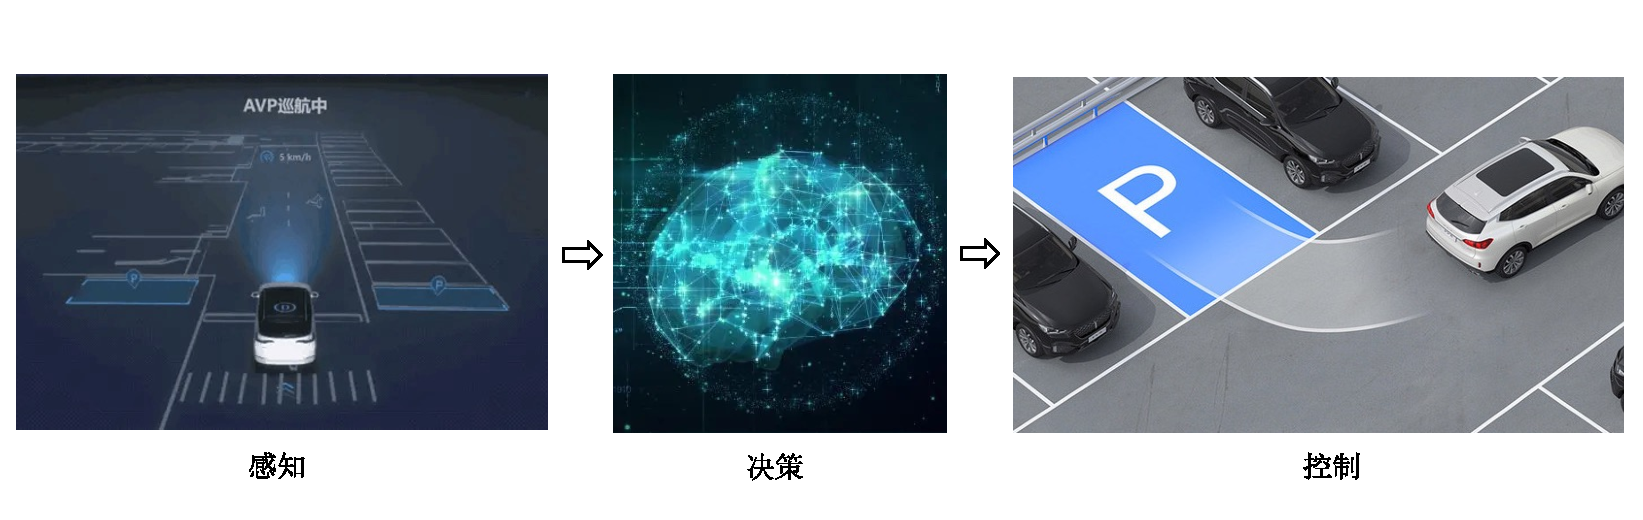
\includegraphics[width=1\linewidth]{figures/chp0/intro.pdf}
  \caption{智能泊车系统示意图  \\Figure~\ref{fig_intro} Architecture of the intelligent parking system}
  \label{fig_intro}
\end{figure}

从目标属性角度来看，停车位并非传统意义上的刚性目标，而是由多条标线和多个关键点共同构成的结构化目标。其几何形态在不同场景中呈现显著差异，例如垂直车位、平行车位和倾斜车位等形式，在关键点分布与结构关系上存在明显不同。此外，停车位通常呈现高密度分布特征，相邻车位之间结构相似，容易在视觉感知过程中产生混淆。这些因素使得停车位检测不仅需要准确的局部特征提取能力，还对模型的结构建模能力提出了更高要求。

从数据获取与模型训练的角度来看，高质量标注数据的获取成本始终是制约停车位检测研究的重要瓶颈。停车位的标注通常涉及多个关键点及其对应关系，标注过程复杂且耗时，难以在大规模、多场景条件下快速扩展。这导致现有公开数据集在规模、场景多样性以及极端复杂条件覆盖方面仍存在不足，进而限制了基于全监督学习方法在真实场景中的泛化能力。如何在有限标注数据条件下充分利用未标注数据，成为停车位检测研究中亟需解决的问题。

在方法设计层面，尽管近年来深度学习技术显著推动了停车位检测性能的提升，但部分现有方法仍沿用“检测 + 后处理”的传统流程，即先预测局部特征或关键点，再通过人工设计的规则对检测结果进行组合与匹配。这类方法在特定场景下能够取得较好效果，但其性能往往依赖于经验性规则与阈值设置，在复杂光照、局部遮挡或停车位密集等情况下容易出现结构不一致或匹配错误的问题。其中，缺乏在模型训练阶段对停车位结构关系的显式建模，是造成上述问题的重要原因之一。

此外，从实际应用场景来看，车辆在泊车过程中获取的是连续的多帧视觉信息，而非孤立的单帧图像。单帧检测方法在面对动态视角变化、短时遮挡以及环境噪声时，容易产生检测结果波动，从而影响系统整体的稳定性与可靠性。然而，现有研究中仍有相当一部分工作主要聚焦于单帧检测任务，未能充分挖掘时序信息在提升停车位检测稳定性方面的潜力。如何将空间结构建模与时间维度信息有机结合，构建更加鲁棒的停车位检测方法，是当前研究中的一项重要挑战。

综上所述，停车位检测在复杂真实场景下仍面临数据受限、结构建模不足以及时序信息利用不充分等问题，亟需从数据、方法建模以及时空融合等多个层面开展系统研究。针对这些问题，本文围绕复杂场景下的停车位检测任务，从数据与学习范式、空间结构感知建模以及多帧时序建模三个层面展开深入研究，具有重要的理论意义与实际应用价值。


\section{研究现状}
\subsection{基于传统算法的停车位检测方法}

（1）基于直线的方法

停车位是停车场内由引导线和分隔线围成的地面区域，主要包括矩形、平行四边形及菱形等多种类型。由于停车位标识由直线段构成，因此直线识别成为停车位检测的关键环节~\cite{ma2021research}。

针对这一关键环节，Jung等人\cite{jung20063d}提出了一种融合像素分类与特征匹配的方法，用于提取停车场的空间结构信息。该方法首先利用平面约束提取停车场标线并转换为俯视图，随后在俯视图基础上通过模板匹配精确定位车位。此外，研究者还利用相邻车辆的视差生成障碍物深度图，通过限定搜索范围与方向，将其作为模板匹配的判别准则。实验结果表明，该方法结合障碍物深度信息与标线俯视图，不仅有效缩小了算法的搜索空间，还显著提升了运算速度及对视觉噪声的鲁棒性。

然而，车载摄像头在光照剧变（如夜间或逆光环境）时的稳健性仍然是一个挑战。针对这一问题，Kamiyama等人\cite{kamiyama2019recognition}提出了一种全天候停车位识别方法，使其在昼夜更替或路面干湿变化的情况下均能正常工作。该方法利用激光测距仪获取接收光强值的统计模型，据此对路面进行分类，并结合霍夫变换（Hough Transform）估计目标停车位置。此外，Jung等人\cite{jung20063d}针对自动泊车辅助系统的车位自动选择问题，提出了一种基于单目视觉的车位线识别算法。该研究在霍夫空间中设计了一维滤波器，利用边缘图像俯视图中车位线特征的先验知识，并引入改进的点到线段距离测度来区分识别出的线段。实验结果表明，即便在相邻车辆严重遮挡车位线的情况下，该算法仍能成功识别车位。

霍夫变换常被用于检测车位标线，但受噪声、杂乱背景、光照波动及天气变化等因素干扰，其在检测平行线对时的稳健性较差，且无法同时检测多个平行线对。针对上述缺陷，Wang等人\cite{wang2014automatic}采用多项式鱼眼畸变模型对摄像头进行标定，并利用基于 Levenberg-Marquardt 算法的图像拼接技术，将四个鱼眼摄像头的图像合成为全向俯视图。在此基础上，该研究引入了基于拉东变换（Radon Transform）的车位特征提取方法，实现了对多个车位的同步检测。此外，文中还指出了其他传感方案的局限性：当超声波传感器的探测距离小于3米时，其测量结果无法为障碍物识别提供有效信息；同时，仅基于后视摄像头的系统由于视野受限，在平行泊车等需要宽阔视野的场景中难以发挥辅助作用。

为了获得更宽阔的视野，研究人员开始探索全景视觉技术在车位检测中的应用。Hamada等人\cite{hamada2015surround}提出了一种基于全景图像的车位检测算法，有效解决了目标车位移出当前视场时的跟踪丢失问题。为提升检测精度，Lee等人\cite{lee2016available}设计了一种锥形帽标线提取滤波器及基于熵的标线聚类算法；即便在能见度较低的情况下，该滤波器仍能强力提取线条特征，随后由聚类算法高效地将特征分配至各车位线段。与霍夫变换等传统线性检测器相比，该方法在处理畸变或模糊标线时速度更快、稳健性更强，且在目标位置与偏航角估计的准确度上优于基于角点检测的方法。

然而，现有方法在处理复杂障碍物干扰和识别微小障碍物方面仍存在不足。针对这些问题，Li等人\cite{li2017automatic}提出了一种基于环视系统（Around View Monitor，AVM）的自动检测方案。该方案利用直线段检测器（Line Segment Detector，LSD\cite{von2012lsd}）在全景图像中识别固定间距的平行标线，并结合图像分割与立体视觉算法计算标线高度，从而识别车位内的细小障碍。实验结果证明，该方法在检测的连续性与完整性上优于霍夫变换，显著降低了误报率与漏检率。在此基础上，Wenhao等人\cite{zong2018robust}对 LSD 算法进行了改进，将其划分为检测与跟踪双线程：检测线程利用改进的提取器获取线段边缘及L型组件结构信息，并结合前后帧关联搜索候选区域；跟踪线程则利用卡尔曼滤波（Kalman Filter）实时更新车位位置并给出置信度评分，最后辅以超声波验证以剔除伪目标。此外，Li等人\cite{li2018geometric}提出的基于几何特征的方法，通过线聚类与几何约束配对，在弱光、强光以及地砖、曲线等复杂路面条件下均表现出优异的全自动检测性能。

为了进一步提升车位检测的自动化程度和稳健性，Jae等人\cite{suhr2018universal}开发了一套全自动化的车位检测与识别方法，该方法能识别多种类型的车位标线，且在不同光照条件下展现出较强的稳健性。首先，该方法从环视系统图像中提取平行线对，以识别车位标线的分割线。随后，将当前帧检测到的分割线与前一帧结果进行融合，并依据车位几何约束对分割线进行配对，从而生成候选车位区域。在此基础上，系统利用直线与角点特征识别车位入口，并配合超声波传感器判断车位占用状态，以对候选车位进行验证。最后，系统将当前帧识别的空闲车位与历史帧结果进行合并，并基于车载运动传感器的里程计数据，实现对历史帧分割线及当前车位位置的持续跟踪。


（2）基于角点的方法

传统的基于直线检测的车位识别方法往往仅能识别一两种特定类型的车位，难以应对现实中如菱形或平行四边形等多样化的车位布局。相比之下，基于角点特征的检测方法能够识别多种车位类型，进而支持更复杂的泊车操作。Suhr等人\cite{suhr2013full}设计了一种全自动车位识别方案，该方案的核心在于将不同类型的车位标线建模为分层树状结构进行识别。该方法主要由“自底向上”与“自顶向下”两个过程组成：首先，通过自底向上的过程逐步生成候选车位；随后，根据车位标线类型的固有属性，沿树状结构自顶向下进行遍历，以剔除虚假车位、冗余节点及干扰角点。最终，系统确定目标车位的准确位置。尽管该方法实现了全自动化，但其在计算量保持较低水平的前提下，性能表现仍显著优于早期的半自动化方法。

在上述研究的基础上，Suhr等人\cite{suhr2013sensor}进一步提出了一套高效的车位检测与跟踪系统，该系统由三个核心阶段组成：在车位标线检测阶段，该研究沿用了文献\cite{suhr2013full}中的分层树状结构方法，实现了对多种车位类型的有效识别。在车位占用分类阶段，系统利用超声波传感器数据判定所检车位的空闲状态。该方法将每个车位区域视为独立的占用栅格单元，并据此计算占用概率。最后，在车位标线跟踪阶段，当车辆驶入车位时，系统会持续估计所选车位的位置。在跟踪过程中，系统在匹配得分层面融合了环视图像与基于运动传感器的测距信息，从而有效应对了车辆入库过程中不可避免的遮挡问题。实验结果表明，该系统能够实时识别各类车位的位置及占用情况，并在实际工况下实现稳定跟踪，既能辅助驾驶员快速选择可用车位，也能通过持续更新目标位置为泊车控制系统提供支持。

传统基于几何特征的方法虽然在特定场景下表现良好，但在处理复杂环境（如严重遮挡、光照变化剧烈等）时仍存在局限性。随着深度学习技术的快速发展，研究人员开始将深度学习算法应用于车位检测任务，以提高检测的鲁棒性和准确性。

\subsection{基于深度学习算法的停车位检测方法}
针对自动车位检测问题，已有大量研究聚焦于环视图像的应用，并由此催生出多种基于深度学习的检测方法。这些方法充分利用了环视图在空间覆盖上的全面性，旨在复杂多变的泊车环境中显著提升检测算法的准确度与稳健性~\cite{aajal2025autonomous}。

（1）基于目标检测的方法

Lin和Huang\cite{zhang2018vision}首次提出了深度停车位检测（DeepPS）方法，该方法基于深度学习，利用深层卷积神经网络（Deep Convolutional Neural Network，DCNN）来检测停车位。该方法对环视图像进行处理，采用两阶段检测流水线来定位和分类停车位特征。在第一阶段，该方法使用预先训练的基于 YOLOv2 的目标检测器识别输入图像中的所有标记点。在第二阶段，使用定制的 DCNN 分析检测到的标记点对，以确定它们是否形成有效的入口线，并将停车位类型分类为垂直、平行或倾斜。根据检测到的标记点和分类输出的空间形状，该方法可以对每个停车位的最终位置和方向进行几何估计。

为了进一步提升车位检测的精度和鲁棒性，Junhao和Zhang\cite{huang2019dmpr}提出了另一种值得注意的方法，名为方向标记点回归（DMPR-PS）。如图 \ref{fig_dmpr} 所示，该算法首先将输入图像送入卷积神经网络（Convolutional Neural Network，CNN）生成特征图；随后，利用这些特征图对定向标线点进行回归，这些点代表了候选车位的角点及其方向信息。接着，车位推断模块对标线点进行配对与筛选，从而锁定最终的车位位置。该方法采用多属性CNN回归模型估计车位的关键特征，包括标线点坐标、车位形状（如T型或L型）、朝向以及检测置信度。最终的车位识别通过一套过滤机制完成，该机制旨在剔除无效的标线点对。例如，同一车位内的两个标线点必须满足预设的最小空间距离阈值，且若两点连线被第三个中间点穿过，则该点对将被视为无效。最后，通过对验证后的定向标线点进行几何配对，形成入口线模式，从而实现对每个独立停车位的精准定位。


\begin{figure}[!h] % use float package if you want it here
%\setlength{\abovecaptionskip}{-0.2cm} %调整图片caption与正文之间的间距，table同理。可自己调整。
  \centering
  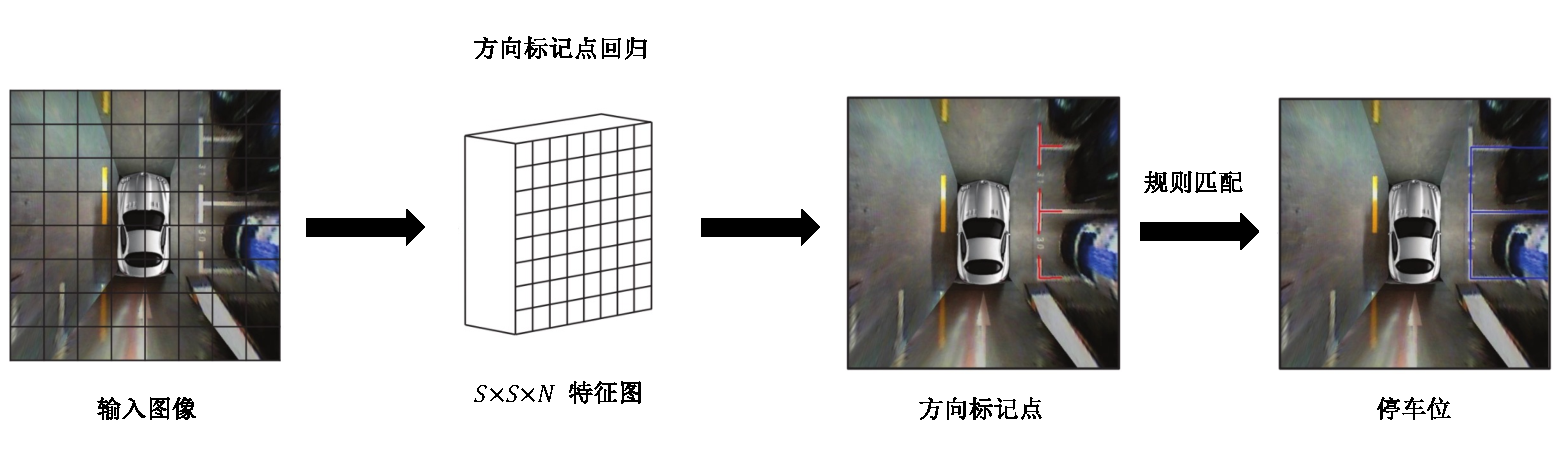
\includegraphics[width=1\linewidth]{figures/chp0/dmpr.pdf}
  \caption{DMPR-PS\cite{huang2019dmpr}算法流程图 \\Figure~\ref{fig_dmpr}~Pipeline of the DMPR-PS\cite{huang2019dmpr}}
  \label{fig_dmpr}
\end{figure}

在车位检测与占用状态识别的结合方面，Li等人\cite{li2020vacant}提出的空闲车位检测网络（VPS-Net）是另一种重要的研究方法。该方法基于YOLOv3\cite{redmon2018yolov3}目标检测模型，通过边界框（Bounding Boxes）对图像中的标线点与车位头进行定位与识别。随后，该系统通过分析成对标线点之间的几何距离以及所识别车位头的构型，推断出车位的具体类型；并进一步应用几何规则推算隐藏角点，从而将检测到的特征关联为完整的车位结构。在车位占用状态的判定上，VPS-Net 引入了基于 AlexNet~\cite{krizhevsky2012imagenet} 架构定制的深度卷积神经网络。与采用单一 CNN 进行检测的 DMPR-PS 不同，VPS-Net 采用了两阶段流水线：第一阶段利用 YOLOv3 检测车位头与标线点，第二阶段则独立对每个检测到的车位进行占用状态分类。

在上述研究的基础上，Wu等人\cite{wu2020psdet}提出的PSDet是一种更为通用且高效的解决方案。该方案采用两阶段级联神经网络架构，并引入了创新的圆形描述符（Circular Descriptor）框架。在第一阶段，该算法从环视输入图像剪裁出的左右子图中提取多尺度特征，随后通过 Softmax 归一化的响应图生成粗略的标线点候选区域。在第二阶段，使用基于 CNN 的精细回归模型对以这些候选区域为中心的小尺寸子图进行处理。在此过程中，圆形描述符被用于估计顶点的精确位置（以偏移量的形式表示）。由于圆形设计本质上具有旋转不变性，该模型能够稳健地应对各类复杂泊车场景中的方向变化。

考虑到模型的训练与推理效率，Li等人\cite{li2020parking}提出了一种深度卷积神经网络架构。该架构引入了定向入口线检测器，旨在估算车位入口线的中点，随后依据预定义的几何规则重构完整的车位几何形状。该定向入口线检测器由30个卷积层组成，并借鉴了 ResNet~\cite{kaiming2016deep} 的设计思路，集成了残差连接。这些残差连接有助于提升梯度流动的效率，从而增强模型的收敛性与训练稳定性。该网络通过预测入口线中点 $P(x,y)$，并根据车位入口的朝向将车位划分为直角、钝角或锐角三类。最后，该系统利用预测的中点坐标与分类结果，通过几何规则推算出车位的最终坐标，实现了对完整停车空间的快速且精准重建。

为了进一步简化检测流程并提高端到端性能，Suhr与Jung\cite{suhr2021end}提出了一种直接作用于环视系统图像的端到端车位检测方法。与早期依赖于节点配对和形状估计等人工几何启发式规则的方法不同，该方法利用卷积神经网络同时提取全局与局部特征。这种集成策略实现了对车位位置、类型、占用状态及节点方向的联合预测，无需复杂的基于规则的后处理过程。该算法首先将输入的AVM图像划分为网格，并利用 CNN 骨干网络（如去掉全连接层的VGG16）提取特征。以$416\times416$的输入尺寸为例，网络生成$13\times13\times512$的特征图，并进一步导出两个独立的输出张量：一个$13\times13\times9$的张量用于表征全局特征（涵盖车位入口、类型及占用情况），另一个$13\times13\times5$的张量用于表征局部特征（捕捉节点的精确位置与朝向）。在此基础上，Bui和Suhr\cite{bui2023cnn}提出了一种专门的两级停车位检测框架，证明了设计良好的两级结构在一般目标检测研究中的性能优于一级模型。在第一阶段，使用区域提案网络（Region Proposal Network，RPN）生成以入口中心、长度和方向为特征的区域提案来检测潜在的停车位入口。在第二阶段，该框架对提案进行细化，以产生停车位属性的精确估计，包括位置、类型和占有率。

Zinelli等人\cite{zinelli2019deep}提出了一种用于环视图像车位检测与占用分类的端到端深度神经网络。该方法基于改进的 Faster R-CNN 架构，并针对泊车环境中常见的几何多变性及斜向视角问题进行了优化。与传统目标检测方法回归轴对齐边界框不同，该模型能够预测通用的四边形框，从而对车位形状进行更灵活、更精确的表征。该架构实现了在各种复杂工况（包括多样的车位形状与朝向）下的稳健检测与分类。由于该模型具备同步进行定位与占用状态评估的能力，使其特别适用于复杂且真实的泊车环境部署。

基于目标检测的方法虽然在检测精度和鲁棒性方面有显著提升，但其依赖大量标注数据进行训练，标注成本较高。这类方法的后处理步骤往往较为复杂，仍需人工设计的几何规则。

% 除了基于目标检测的方法外，图像分割技术也在车位检测中得到了广泛应用，为识别车位标线提供了更精细的像素级信息。

（2）基于图像分割的方法

基于深度学习的车位检测方法广泛利用图像分割技术来识别并定位关键视觉特征。其中，语义分割（Semantic Segmentation）技术常用于对图像中的每个像素进行分类，从而有效区分车位标线与背景，并提供关于标线位置与形状的详细信息。与之不同，实例分割（Instance Segmentation）方法，尤其是基于 Mask R-CNN~\cite{he2017mask} 架构的方案，则侧重于检测并生成特定标线点（如T型或L型节点）的精确掩码，进而界定车位边界。

Jiang等人\cite{jiang2020detection}提出了一种集成深度学习与经典计算机视觉技术的车位检测方法。该方法采用以 ResNet-101 和特征金字塔网络（Feature Pyramid Network，FPN）为骨干网络的 Mask R-CNN 模型，通过生成实例分割掩码来检测T型和L型等交叉节点。在预处理阶段，该系统通过感兴趣区域选择与对比度增强提升图像质量；在检测完成后，该系统利用形态学操作对掩码进行细化，并结合 LSD 算法提取结构线与引导线。最终，该系统依据标线点分类结果与几何先验推断出车位的朝向与深度。尽管该方法在精度上有所提升，但其对 LSD 算法的依赖导致在直线检测效率方面存在不足。

为了提高环视图像的分割精度并减少对传统算法的依赖，Wu等人\cite{wu2018vh}提出了一种 VH-HFCN 网络，专门用于检测全景环视图像中的车位与车道线。该网络架构基于高度融合卷积网络（Highly Fused Convolutional Network，HFCN），并在上采样阶段前引入了“VH阶段”：该阶段由两个并行的卷积分支组成，分别采用垂直（$9\times1$）和水平（$1\times9$）卷积核。这一设计显著增强了网络对线性特征的提取能力。在分割任务完成后，该算法通过三个步骤进行后处理：首先，利用形态学骨架化提取中心线；然后，应用霍夫变换进行直线检测；最后，利用基于相似性的合并算法重构完整的车位几何形状。

与依赖几何模型的方案不同，Jang与Sunwoo\cite{jang2019semantic}提出了一种统一的感知系统，该系统能够在不依赖人工设计特征的前提下，同步检测车位标线与静态障碍物。该框架主要包含两个阶段：a. 语义分割阶段：采用具备编码器-解码器（Encoder-Decoder）结构的全卷积网络，将环视图像中的每个像素划分为四类：空闲空间、车位标线、车辆以及其他静态物体（如墙壁、路缘、柱子等）。b. 基于垂直栅格的检测阶段：对分割结果进行二值化、垂直编码、聚类及精细化处理。具体而言，该系统利用最优阈值对特定类别的分割图进行二值化，并采用垂直栅格编码技术将数据抽象为水平向量。随后，该系统通过对空单元格进行聚类以识别候选车位，最后通过精细化步骤估计每个车位的位置与朝向。这种基于栅格的后处理方式实现了高效且结构化的车位检测，无需传统的直线拟合或人工定义的启发式规则，使其非常适用于自动泊车系统的实时应用场景。

基于图像分割的方法虽然能够提供精细的像素级信息，但其计算复杂度较高，实时性表现较差。这类方法对标注数据的质量要求更高，后处理步骤也较为复杂，需要额外的几何约束，在低对比度或模糊场景下分割精度容易下降。

（3）基于结构化建模的方法

现有的许多用于停车位检测的深度学习方法依赖于复杂的后处理步骤，这既耗时又容易导致结果不准确。为解决这些问题，Min等人\cite{min2021attentional}提出了一种基于注意图神经网络（Attention-based Graph Neural Network，AGNN~\cite{thekumparampil2018attention}）的端到端可训练方法，消除了人工设计的后处理步骤。他们方法的核心思想是将环视图像中的标记点（即停车位的角点）表示为图结构的数据集。该模型利用图神经网络（Graph Neural Network，GNN\cite{scarselli2008graph}）对相邻标记点的上下文信息进行聚合，通过关系推理实现更准确的车位检测。该框架由三个主要模块组成：a. 图形特征编码器：AGNN 从环视图像中提取深层特征，以检测标记点位置并生成特征描述符。位置信息通过多层感知器（Multilayer Perceptron，MLP）嵌入，并与外观特征融合。b. 图特征聚合：构造一个全连通图，每个节点对应一个检测到的标记点。基于注意力的多头 GNN 聚集相邻节点的特征，捕捉几何和上下文依赖关系。c. 入口线鉴别器：对于一对标记点，它们的融合特征被串联并通过基于MLP的鉴别器，该鉴别器预测该对是否构成停车位的有效入口线。该方法在简化推理流水线的同时，避免了额外的后处理过程，具有较好的性能。

在结构化建模的基础上，Bui与Suhr\cite{bui2023transformer}进一步提出了一种专门针对车位检测设计的 Transformer~\cite{vaswani2017attention} 框架。尽管如检测 Transformer（DETR\cite{carion2020end}）等架构在通用目标检测中展现出巨大潜力，但由于训练时间长且车位表征能力欠佳，其在车位检测中的直接应用受到了限制。为此，该研究引入了多项改进：首先，借鉴 Anchor DETR\cite{wang2022anchor}的思路，采用固定锚点取代了 DETR 中的可学习目标查询（Object Queries）；每个锚点对应特征图中预定义的空间区域，从而减少了预测歧义并加速了模型收敛。其次，模型提出了一种创新的“两点式车位表征法”，即仅通过入口节点的坐标与朝向来定义车位。这种表征方式特别适用于环视系统图像，因为在实际场景中，AVM 往往只能捕捉到车位的部分视图。该 Transformer 架构保留了 DETR 的编码器-解码器结构，但在效率与精度上均有提升。与传统模型不同，该方法无需非极大值抑制（Non-Maximum Suppression，NMS）等后处理技术，进一步简化了算法流程。实验结果证实，该模型性能优于早期的 Transformer 方案，并能与当前顶尖的基于 CNN 的检测器相媲美。

基于结构化建模的方法虽然在端到端性能和结构推理方面有优势，但其计算复杂度较高，模型训练成本较大。这类方法对标记点检测精度要求较高，容易受到噪声影响。并且，在密集停车位场景中，图结构复杂度增加，最终会导致推理速度下降。



（4）基于多视角与大模型先验的方法

随着大视觉模型和多视角技术的发展，研究人员开始探索新的车位检测方法，以进一步提升检测性能和泛化能力。Zhai等人\cite{zhai2024sam}于2024年提出了基于大视觉模型的停车位检测方法 SAM-PS，首次将分割一切模型（SAM\cite{kirillov2023segment}）应用于该任务，解决了传统方法鲁棒性不足、深度学习方法依赖训练数据的问题，实现了零样本检测。该方法以环视图像为输入，采用两阶段架构：第一阶段通过 SAM 模型生成多掩码，无需人工提示；第二阶段经多掩码过滤（按面积阈值筛选+角点模板匹配）提取有效掩码，再通过距离约束与四类停车位模板（含新增YY型适配斜列停车）完成定位，全程无需训练。

针对传统基于 AVM 图像的检测方法易受畸变、遮挡影响，且多数方法忽视停车位整体结构的核心问题，Duan等人\cite{duan2025bev}于2025年进一步提出了基于 BEV（Bird's Eye View）和多边形建模的端到端停车位检测框架 BEV-PolyNet。该框架以环视鱼眼图像为输入，核心包含四大模块：a. 数据处理模块对鱼眼图像去畸变、IPM（Inverse Perspective Mapping） 投影拼接生成 AVM 图像；b. BEV 模块通过 ResNet-34 和 FPN 提取图像特征，经视图变换生成BEV特征，从根源上规避 AVM 图像的畸变与视野局限；c. 查询初始化模块利用AVM图像特征和预设停车位尺寸先验初始化查询向量，并融入位置编码以加速模型收敛；d. 解码与预测模块通过可变形解码器和迭代优化策略，以多边形形式精准回归停车位四角坐标并完成分类。该方法能够灵活适配平行、垂直、倾斜及不规则等多种形状停车位，在ps2.0、PSDD公开数据集及私有LPD数据集上均表现出优异的检测精度与泛化能力，为复杂场景下的停车位检测提供了新的有效方案。

基于多视角与大模型先验的方法虽然在泛化能力和鲁棒性方面有显著提升，但由于大模型推理成本较高，难以在边缘设备上实时部署。这类方法对硬件资源要求较高，计算复杂度较大。并且多视角融合过程也较为复杂，容易引入额外误差，在复杂场景下表现不够稳定。

通过对现有停车位检测方法的全面分析，不难发现，当前研究仍面临一些挑战。首先，现有公开数据集在规模、场景多样性以及极端复杂条件覆盖方面仍存在不足，且高质量标注数据获取成本高，限制了模型的泛化能力。其次，尽管深度学习方法在检测精度上有显著提升，但多数方法仍依赖人工设计的后处理规则，缺乏对停车位结构关系的显式建模，导致其在复杂与密集场景下的结构一致性难以保证。同时，现有研究中仍有相当一部分工作主要聚焦于单帧检测任务，未能充分挖掘时序信息在提升停车位检测稳定性方面的潜力，在动态视角变化、短时遮挡以及环境噪声时容易产生检测结果波动。

针对这些挑战，本文围绕复杂场景下的停车位检测任务，从数据构建与半监督学习、空间结构感知建模以及多帧时序融合三个层面展开深入研究，旨在提出更加鲁棒、高效的停车位检测方法。




\section{主要研究内容}

围绕复杂场景下停车位检测任务中数据受限、结构表达不足以及连续场景下检测稳定性不足等问题，本文从数据构建与学习范式设计、单帧结构感知检测方法以及多帧时序特征融合方法三个方面展开研究，主要研究内容如下：

（1）构建复杂真实场景停车位检测数据集并提出半监督学习方法。针对现有停车位检测数据集规模有限、复杂场景覆盖不足的问题，本文构建了一个覆盖多光照、多场景和多停车形式的大规模停车位数据集 CRPS-D。并在此基础上，设计了一种面向停车位检测任务的半监督检测方法 SS-PSD，通过教师–学生学习范式充分利用未标注数据，有效提升模型在复杂场景下的泛化能力。

（2）提出面向结构感知的停车位关键点检测与匹配方法。针对传统方法中依赖启发式规则进行后处理匹配、结构一致性难以保证的问题，本文提出了一种空间结构感知的端到端停车位检测方法。该方法以关键点表示为核心，在端到端训练过程中显式引入停车位结构关系约束，实现关键点定位与结构匹配的联合优化，从而提升复杂与密集场景下停车位检测的稳定性与一致性。

（3）提出面向多帧时序信息融合的停车位检测方法。针对真实驾驶场景中连续帧条件下检测结果易受遮挡和视角变化影响的问题，本文提出了一种多帧时序信息融合的停车位检测方法。通过融合连续帧中的结构感知表示，实现对停车位时序一致性的建模，有效提升了检测结果在时间维度上的鲁棒性与检测稳定性。

如图 \ref{fig_arch} 所示，本文的研究工作呈现逐步递进关系：首先构建数据集并设计半监督方法，然后在此基础上提出空间结构感知的端到端检测框架，最后进一步引入时序信息提升模型在复杂场景下的稳定性与鲁棒性。

\begin{figure}[!h] % use float package if you want it here
%\setlength{\abovecaptionskip}{-0.2cm} %调整图片caption与正文之间的间距，table同理。可自己调整。
  \centering
  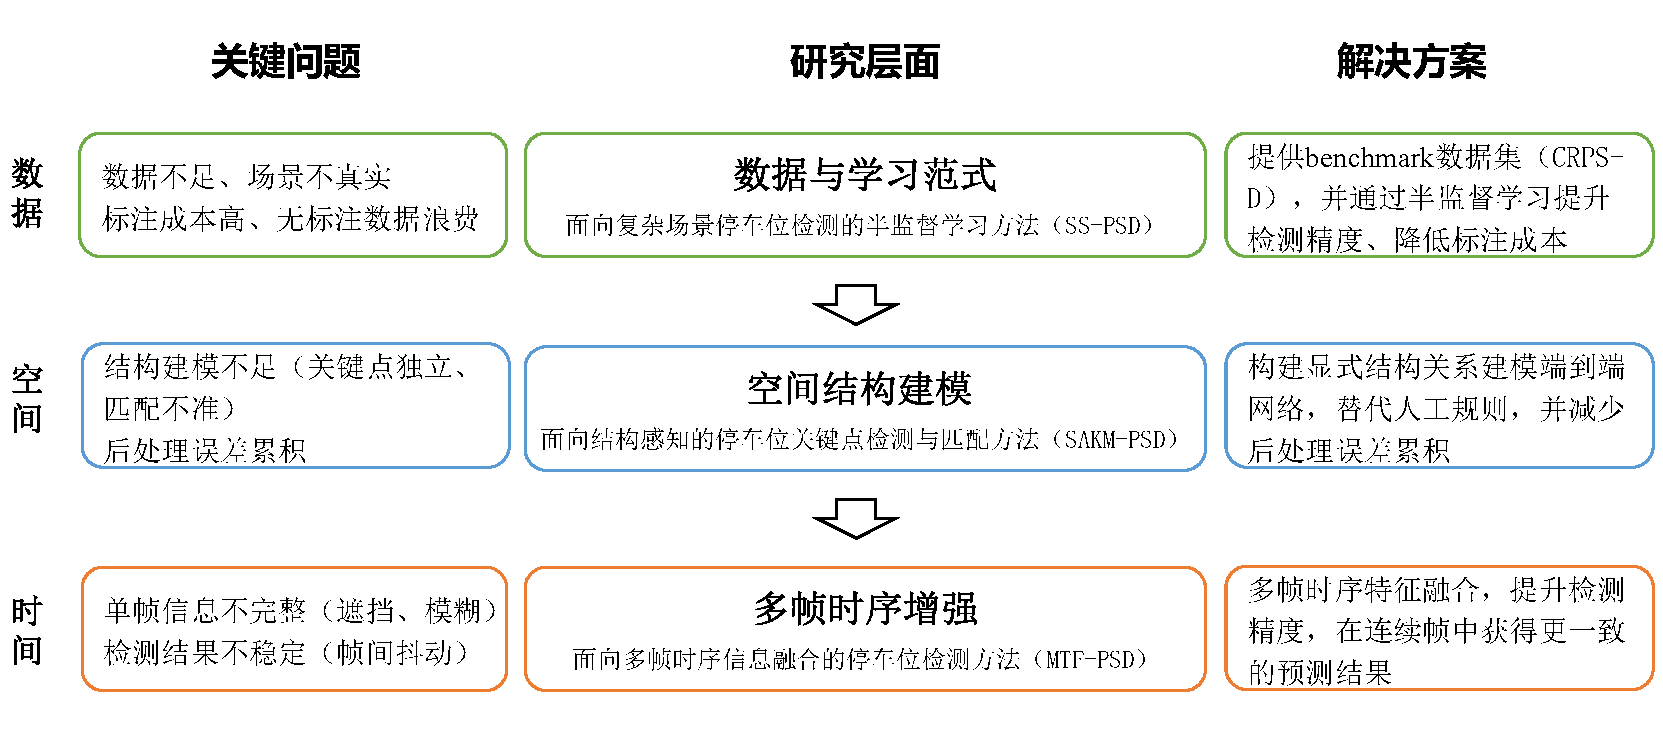
\includegraphics[width=1\linewidth]{figures/chp0/arch.pdf}
  \caption{论文研究内容  \\Figure~\ref{fig_arch}~Research content of the thesis}
  \label{fig_arch}
\end{figure}

\section{论文组织结构}

本章的整体结构安排如下：

第一章 绪论，本章介绍了研究背景与意义，分析了停车位检测在自动泊车系统中的关键作用，并总结了当前停车位检测技术面临的数据受限、空间结构建模不足以及时序信息利用不充分等挑战。并明确了本文的研究目标与主要贡献，概述了论文的整体组织结构。

第二章 相关理论，本章介绍了停车位检测领域通用框架、现有公开数据集、相关评价指标，以及半监督学习、注意力机制和时序建模的理论基础，为后续研究提供理论支撑。

第三章 面向复杂场景停车位检测的半监督学习方法，本章介绍了包含 35739 张图像的真实场景停车位检测数据集 CRPS-D，并对其特点进行定性与定量分析。同时提出了基于教师-学生架构的半监督学习框架 SS-PSD，通过置信度引导掩码一致性与自适应特征扰动机制挖掘无标签数据的空间先验，最后，通过多个实验验证了半监督学习在停车位检测中的有效性。

第四章 面向结构感知的停车位关键点检测与匹配方法，本章介绍了双分支检测框架 SAKM-PSD，包含结构感知 CutMix 策略、注意力引导插值模块与稀疏对匹配损失，实现了关键点定位与结构匹配的联合优化，增强模型对结构信息的感知能力与鲁棒性。最后，在ps2.0和 CRPS-D 数据集上验证了方法的有效性。

第五章 面向多帧时序信息融合的停车位检测方法，本章介绍了时序框架 MTF-PSD ，包含跨帧自注意力机制、动态结构感知时序融合模块及时序鲁棒增强策略，实现了时空联合感知的停车位检测。同时为了进一步评估方法的有效性，提出了PSTD 时序数据集，通过实验验证了多帧时序融合对检测性能的提升。最终，分析了 MTF-PSD 模型在实际车载平台上的推理效率。

第六章 总结与展望，本章总结了本文的主要工作与创新点，分析了所提出的方法在复杂场景下的优势与局限性，并展望了未来的研究方向，包括模型轻量化、多模态融合及端到端自动驾驶系统集成等。

 								%引言
    %   \setlength{\baselineskip}{20pt}
\chapter{相关理论}
\label{cha:chap3}
本章对停车位检测领域的现有数据集及一般方法进行系统归纳与讨论，为后续研究提供理论基础。图\ref{fig_dataset}直观展示了不同研究方法的分布比例以及各数据集的使用情况。

\section{公开数据集}
（1）ps2.0数据集

ps2.0数据集由同济大学的Zhang等人\cite{zhang2018vision}提出，是车位检测领域应用最为广泛的数据集之一。该数据集包含 9827 张训练图像和 2338 张测试图像，所有图像的分辨率均为 $600 \times 600$ 像素。ps2.0 通过对四路鱼眼摄像头获取的图像进行拼接，生成了鸟瞰图（BEV）表征。该数据集涵盖了极其多样的停车场环境，包括室外和室内场景，并包含三种不同的车位类型。研究人员广泛利用该数据集对各自的车位检测方法进行评估与基准测试，并取得了卓越的精度，许多研究报告的查准率已达到99\%左右。


（2）PSV数据集

PSV数据集由Wu等人\cite{wu2018vh}提出，通过同济大学智能电动车（TiEV）平台在同济大学嘉定校区的道路环境下采集而成。它包含2550张训练图像、425张验证图像以及1274张测试图像，所有图像分辨率均为$640 \times 480$像素。该数据集的图像同样通过四路鱼眼摄像头采集，并经过拼接处理生成鸟瞰图。起初，该数据集主要针对图像分割方法的训练而设计，后续通过添加针对目标检测的标注格式，也可用于训练目标检测模型。

（3）SNU数据集 

SNU数据集由首尔大学Do和Choi\cite{do2020context}发布，包含18,299张训练图像和4,518张测试图像，分辨率均为$768 \times 256$像素。SNU数据集旨在提供更丰富的场景和多样化的车位类型，作为ps2.0数据集的优选替代方案。在采集过程中，鱼眼摄像头被安装在车辆侧面，采集到的图像未进行拼接处理，允许检测算法直接处理单个摄像头的原始图像，无需进行图像拼接。尽管SNU数据集已成为ps2.0数据集的一种有潜力的替代方案，但其在停车位检测研究中的应用仍相对有限。

\begin{figure}[!h] % use float package if you want it here
%\setlength{\abovecaptionskip}{-0.2cm} %调整图片caption与正文之间的间距，table同理。可自己调整。
  \centering
  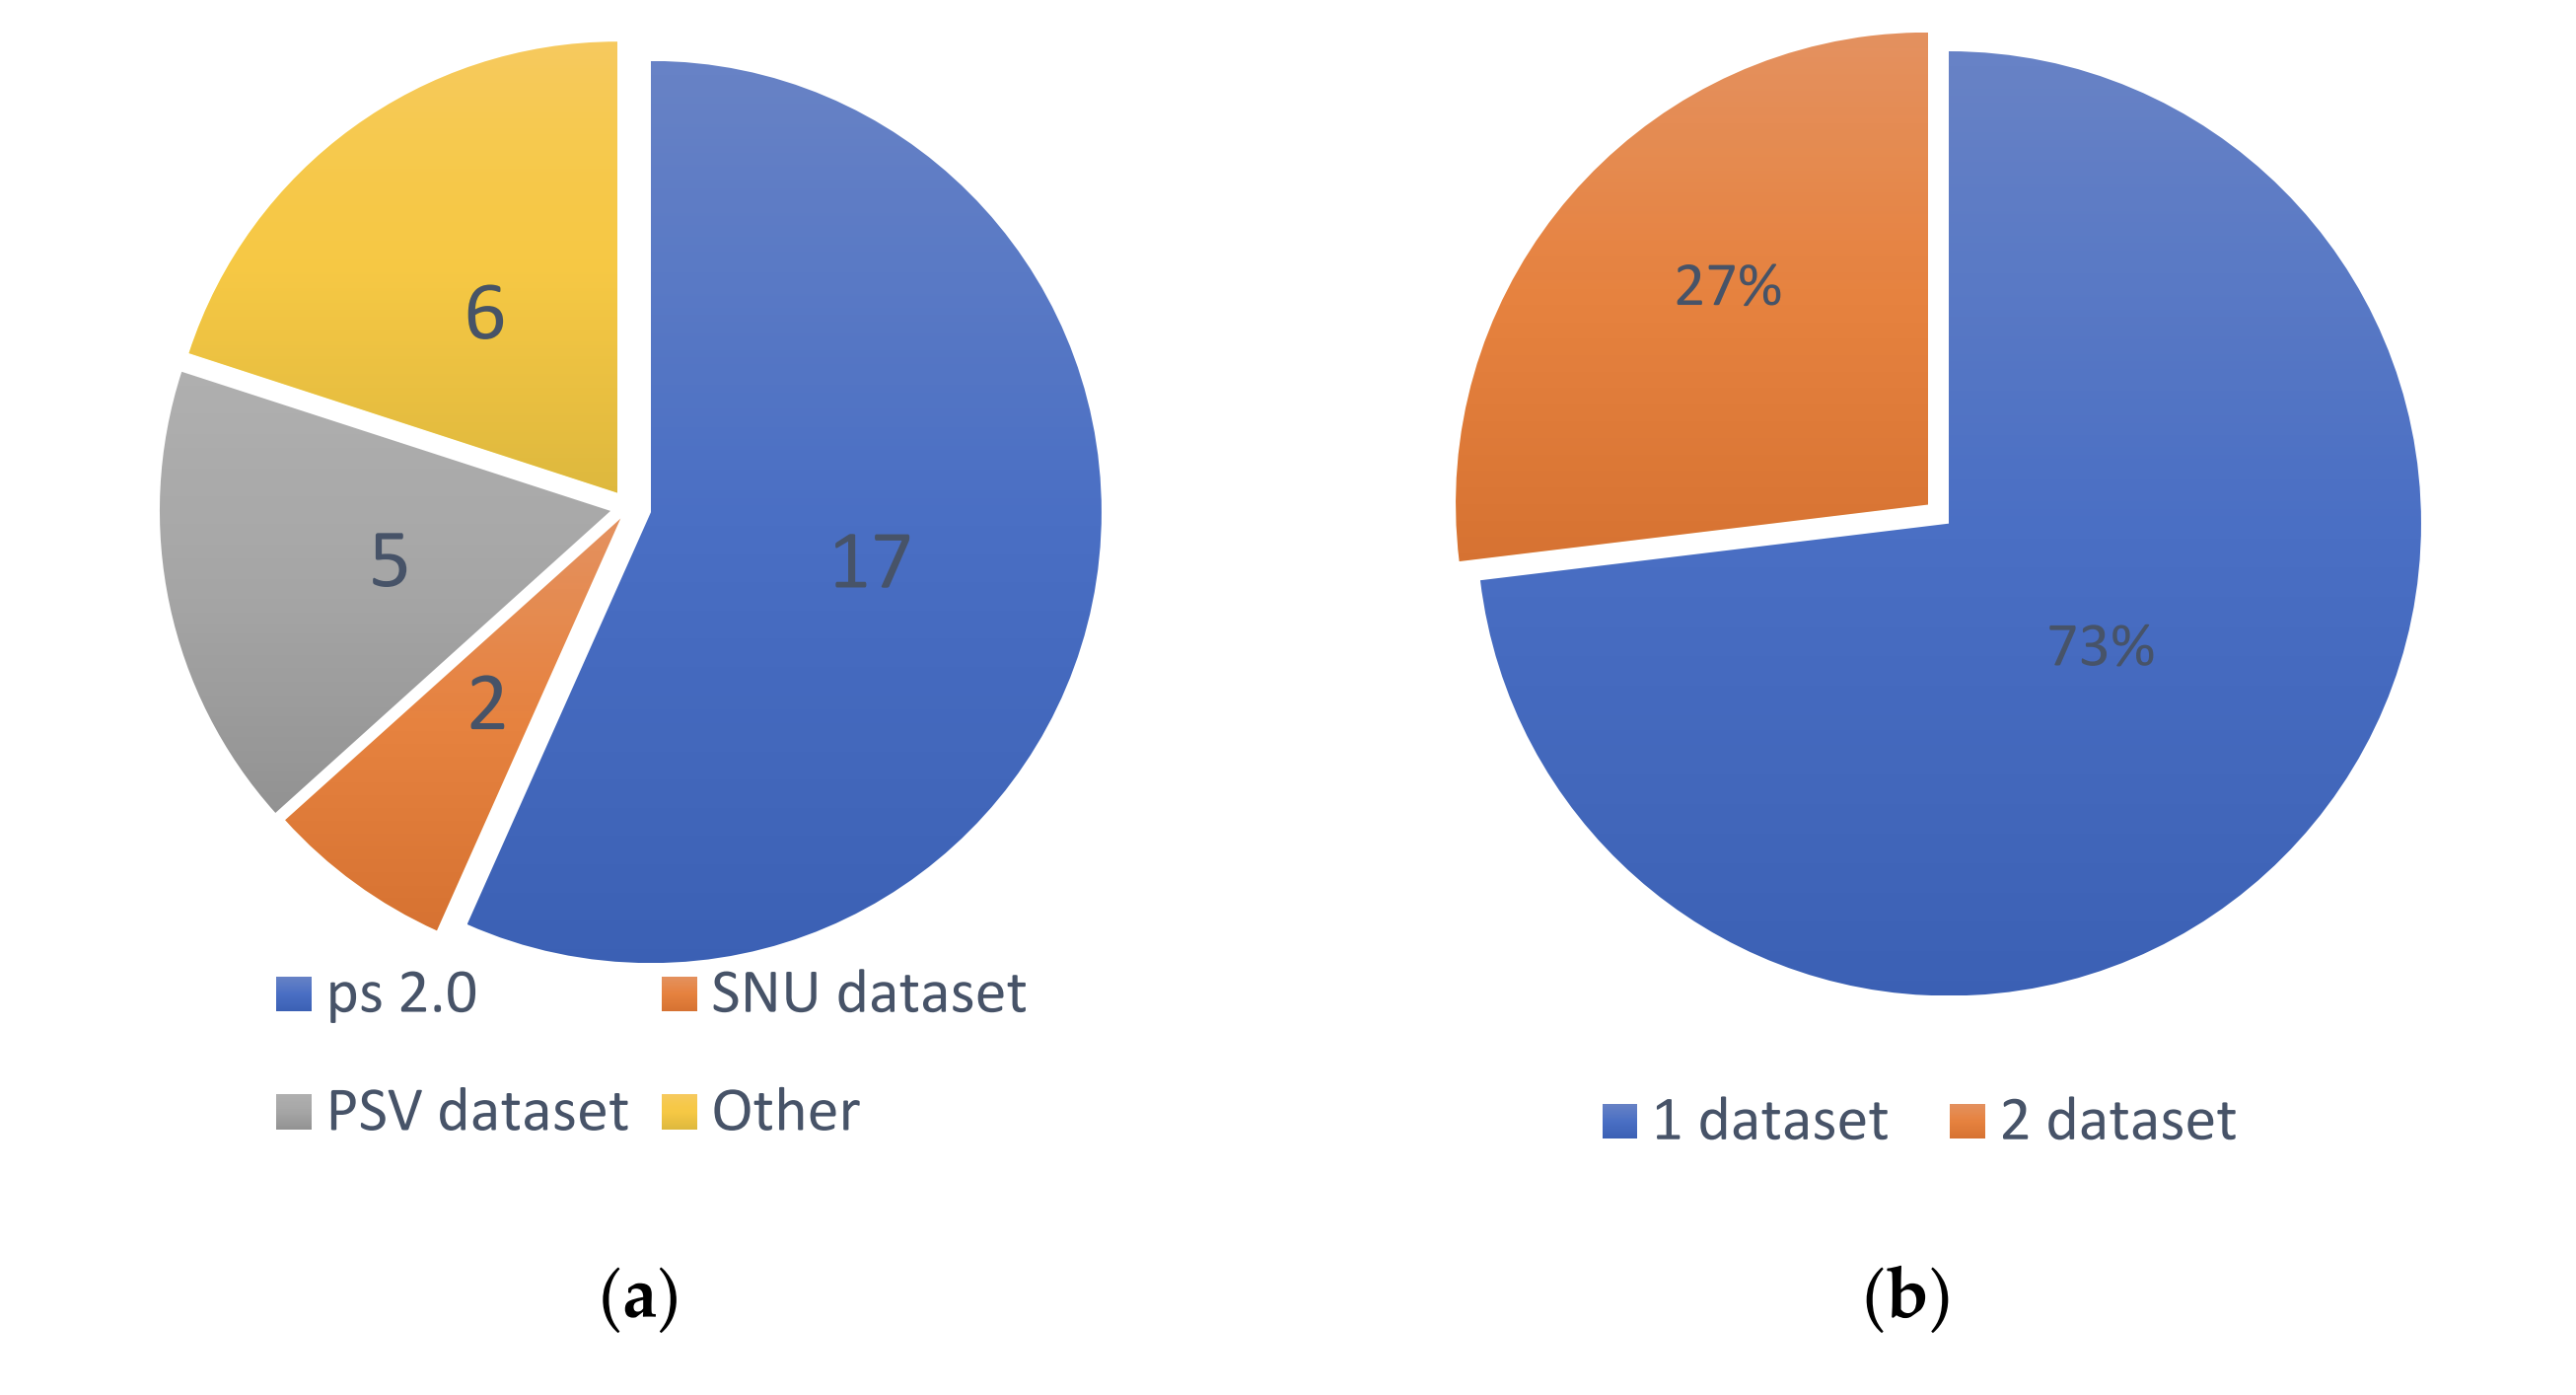
\includegraphics[width=1\linewidth]{figures/chp1/datasets.png}
  \caption{数据集使用分布情况\cite{wong2023review} \\Fig~\ref{fig_dataset}~Dataset Distribution\cite{wong2023review}}
  \label{fig_dataset}
\end{figure}

图\ref{fig_dataset}（a）展示了所综述作品中数据集的使用分布情况。观察可见，大多数研究（共17项）选择利用ps2.0数据集来评估其方法。此外，有6项研究采用了自行采集且未公开的数据集（标注为"其他"）。而2020年发布的SNU数据集在方法评估中的使用相对有限（仅2项研究）。

图\ref{fig_dataset}（b）描绘了关于所使用数据集数量的评估策略。多数研究（73\%）依赖单一数据集来评估其算法。然而，有27\%的研究在评估中采用了两个数据集，包括将一个公开数据集与另一个自标注数据集相结合，或是同时利用两个公开数据集。采用多个数据集进行评估代表了一种更有前景的研究方向，因为它能够验证方法在不同数据集之间的泛化能力。


\section{停车位检测一般方法}

如图\ref{fig_pip1}所示，停车位检测的典型流程包括以下几个关键环节：首先，输入图像通常是由全景环视系统（AVM）生成的环视图，或是由鱼眼摄像头直接捕捉的鱼眼图像。在送入特征提取骨干网络之前，输入图像需经过预处理步骤，如尺寸调整（Resizing）以及翻转、添加噪声等数据增强技术，以提升模型的鲁棒性。

特征提取模块在停车位检测中起着核心作用，负责提取从低级到高级的特征表示。低级特征包括角点或颜色信息，用于捕捉停车位的局部细节；高级特征则代表更抽象的语义信息，如停车位的整体形状、尺寸及排列布局。

提取出的特征随后被传递至检测、分类或分割模块以生成预测结果。输出预测可以采取多种形式，例如标线点坐标、停车位区域边界，或是代表车位边界的分割掩码。为了优化预测输出，系统通常会利用预定义的几何规则或模板匹配技术进行后处理，确保预测结果符合停车位的预期几何特征。


\begin{figure}[!h] % use float package if you want it here
%\setlength{\abovecaptionskip}{-0.2cm} %调整图片caption与正文之间的间距，table同理。可自己调整。
  \centering
  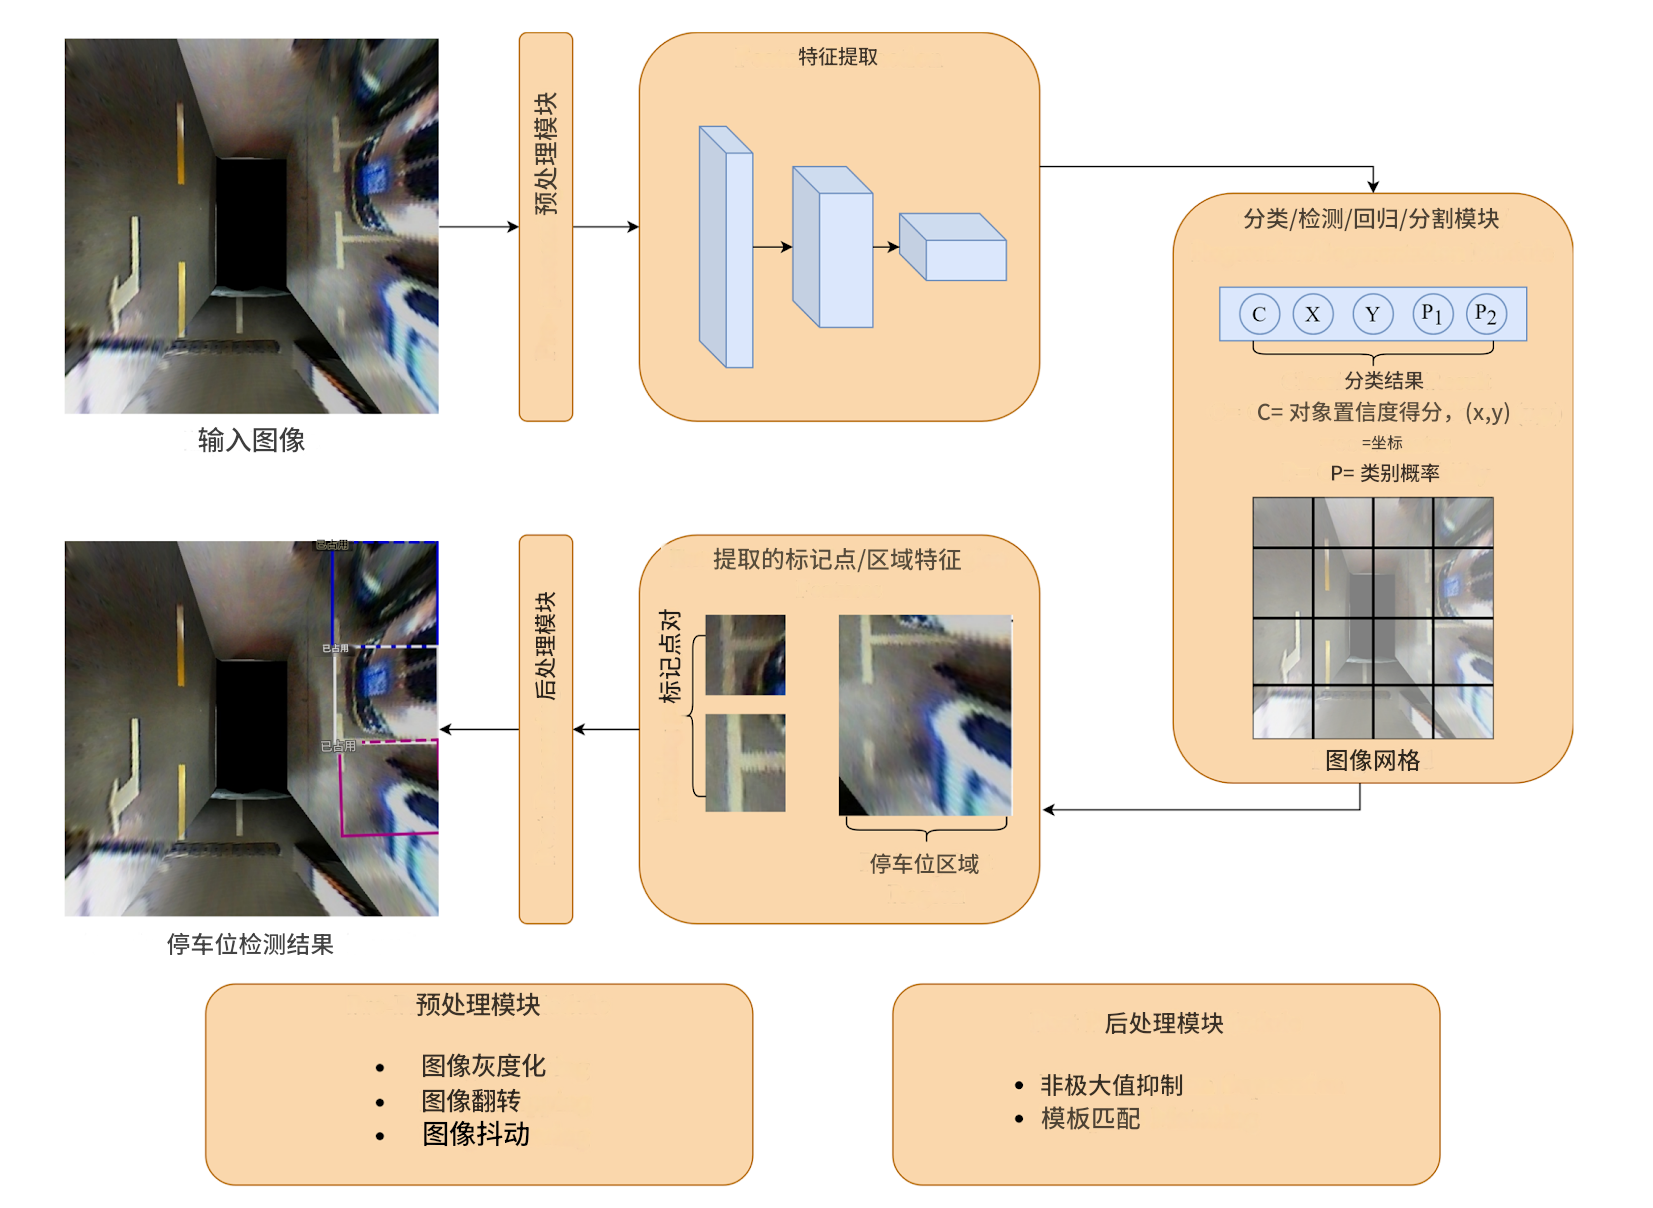
\includegraphics[width=1\linewidth]{figures/chp1/pipline.png}
  \caption{停车位检测的一般流程\cite{wong2023review} \\Fig~\ref{fig_pip1}~General Flow for Parking Slot Detection\cite{wong2023review}}
  \label{fig_pip1}
\end{figure}


\section{模型评估指标}

在停车位检测研究中，传统评估指标多采用查准率（Precision）和查全率（Recall）。然而，这两个指标对阈值选择较为敏感，可能影响评估结果的可靠性。为提供更全面的评估，本文采用平均精度（Average Precision, AP）作为主要评估指标，具体应用\textit{PASCAL VOC 2010}中的全点插值方法，计算方式如下：

\begin{equation}
AP = \sum \Big((Recall_{j+1}-Recall_{j}) \times Precision_{j+1} \Big)
\end{equation}

其中 $j$ 是满足 $Recall_{j} \neq Recall_{j+1}$ 的索引。

查准率和查全率的计算公式如下：

\begin{equation}
Precision = \frac{TP}{TP + FP}
\end{equation}

\begin{equation}
Recall = \frac{TP}{TP + FN}
\end{equation}

式中，$TP$（True Positives）表示正确检测出的真实目标数量，$FP$（False Positives）表示误报为目标的背景区域数量，$FN$（False Negatives）表示未被检测出的真实目标数量。

为明确TP的判定标准，本文将标记点定义为$P=\{x, y, s, t, \theta_{1}, \theta_{2}\}$，其中$(x, y)$表示标记点位置，$s$表示形状，$t$表示类型，$\theta_{1}, \theta_{2}$表示两个边缘的角度（以度为单位）。设$P^{g}=\{x^{g}, y^{g}, s^{g}, t^{g}, \theta_{1}^{g}, \theta_{2}^{g}\}$为真实标记点（Ground Truth），$P^{d}=\{x^{d}, y^{d}, s^{d}, t^{d}, \theta_{1}^{d}, \theta_{2}^{d}\}$为检测到的标记点。当满足以下条件时，认为$P^{g}$被准确识别，$P^{d}$为TP：

\begin{subequations}
  \begin{align}
  (x^{g}-x^{d})^{2} + (y^{g}-y^{d})^{2} < I^{2} \\
|\theta_{1}^{g} - \theta_{1}^{d}| < B \ or \ 360^{\circ} - |\theta_{1}^{g} - \theta_{1}^{d}| < B \\
|\theta_{2}^{g} - \theta_{2}^{d}| < B \ or \ 360^{\circ} - |\theta_{2}^{g} - \theta_{2}^{d}| < B \\
s^{g} = s^{d} \ and \ t^{g} = t^{d}
  \end{align}
  \end{subequations}
  
如果满足这些条件，可以认为 $P^{g}$ 被准确识别，并且 $P^{d}$ 为TP。

本文将停车位定义为 $S=\{(x_{1}, y_{1}), (x_{2}, y_{2}), \theta_{s}\}$，其中 $(x_{1}, y_{1})$ 和 $(x_{2}, y_{2})$ 是两个标记点的坐标，$\theta_{s}$ 表示入口线的方向。对于一个 GT 停车位 $S_{g}=\{(x_{1}^{g}, y_{1}^{g}), (x_{2}^{g}, y_{2}^{g}), \theta_{s}^{g}\}$，如果检测到的停车位 $S_{d}=\{(x_{1}^{d}, y_{1}^{d}), (x_{2}^{d}, y_{2}^{d}), \theta_{s}^{d}\}$ 满足以下等式，则将其视为TP：
\begin{subequations}
  \begin{align}
  (x_{1}^{g}-x_{1}^{d})^{2} + (y_{1}^{g}-y_{1}^{d})^{2} < I^{2} \\
(x_{2}^{g}-x_{2}^{d})^{2} + (y_{2}^{g}-y_{2}^{d})^{2} < I^{2} \\
|\theta_{s}^{g} - \theta_{s}^{d}| < B \ or \ 360^{\circ} - |\theta_{s}^{g} - \theta_{s}^{d}| < B
  \end{align}
  \end{subequations}

即当停车位的两个标记点均位于真实停车位（GT）的$I$个像素范围内，且$S_{d}$与$S_{g}$的角度差小于$B$时，判定为真阳性。对于$512 \times 512$分辨率的图像，通常设定$I=10$，$B=30$。
% 对于 ps2.0，$I=10$；对于 CRPS-D，$I=8.53$，从 $10 \times \frac{512}{600}$ 调整，以适应较小的图像尺寸 $512 \times 512$。

\section{本章小结}

本章系统梳理了停车位检测领域的核心理论基础，为后续研究提供了坚实支撑。具体内容包括：

首先，详细介绍了ps2.0、PSV、SNU三个主流公开数据集，分析了各数据集的图像特征、标注方式及研究应用情况。其中，ps2.0数据集应用最为广泛，SNU数据集作为新兴替代方案展现出一定潜力，但应用仍相对有限。

其次，阐述了停车位检测的通用流程，涵盖图像输入、预处理、特征提取、检测分割及后处理等关键环节，明确了各模块的功能与作用，为后续方法设计提供了参考框架。

最后，定义了模型评估指标体系，重点介绍了平均精度（AP）的计算方法，并详细界定了标记点和停车位的真阳性判定标准，为后续算法评估提供了统一、客观的基准。

通过本章的理论铺垫，为后续章节的方法设计与实验验证奠定了坚实的基础。 
     \setlength{\baselineskip}{20pt}
\chapter{大规模停车位数据集构建与半监督检测框架}
\label{cha:chap2}

\section{研究动机}
自动泊车技术在自动驾驶领域占据着不可或缺的重要地位。精准的停车位检测作为自动泊车系统的关键起始环节，对后续车辆规划有着直接影响。在此情形下，环视摄像头系统成为首选解决方案，它能够提供车辆周围环境的全景鸟瞰图，从而更高效地实现停车位检测。传统停车位检测方法严重依赖手工提取的特征，诸如拐角与线条等，这些方法远不能达到令人满意的精度，特别是在几何特征匮乏的场景中。 

随着各类基于深度学习的目标检测技术不断发展，基于学习的停车位检测算法如今已取代传统方法。首个基于学习的算法DeepPS\cite{zhang2018vision}及其基准数据集ps2.0的问世，极大地推动了该领域的进步。此后，研究人员通过标记点回归\cite{huang2019dmpr}、图神经网络GNN\cite{min2021attentional}以及基于Transformer的方法\cite{bui2023transformer}等多种途径，致力于提升检测精度。近期，这些算法在基准数据集ps2.0上取得了先进性能，查准率超99\%。然而，现实停车场景往往更为复杂棘手。当这些解决方案应用于实际自动泊车场景时，常常难以达到预期性能。因此，构建一个规模更大、挑战性更强且更贴合实际的数据集迫在眉睫，这对于推进实际停车位检测以及完善算法可行性评估意义重大。 

为满足上述需求，本文收集并标注了一个大规模真实场景数据集，命名为CRPS-D\cite{zhang2025advancing}，用于车位检测任务。该数据集涵盖地上停车场、地下停车建筑、路边停车区等多种车位类型，旨在囊括城市环境中各类真实泊车场景。数据采集覆盖不同时间段及各种天气条件，如白天、黑夜、晴天、阴天与雨天。据本文所知，该数据集在规模上远超所有公开数据集（如ps2.0\cite{zhang2018vision}和SNU\cite{do2020context}）。此外，相较于这些数据集，CRPS-D具有更高的车位集中度、更多的斜向车位示例以及更复杂的道路场景。这些因素共同提升了车位检测的复杂度，提供了一个全面且极具挑战性的基准，有力推动真实场景下车位检测技术的发展。 

另一方面，本文观察到在真实场景中，停车位检测方法的性能在很大程度上取决于训练数据的规模与多样性。然而，停车位作为典型的结构化目标，其标注过程通常涉及多个关键点及其结构关系，标注成本高、周期长，导致现有公开数据集在规模和场景覆盖方面普遍存在欠缺。这使得基于全监督学习的停车位检测方法在面对复杂光照、多视角变化以及非标准停车形式时，泛化能力明显受限。 

为缓解标注数据受限对模型训练的影响，近年来半监督学习在目标检测等任务中逐渐受到关注。通过引入未标注数据参与模型训练，半监督学习能在一定程度上降低对人工标注的依赖。然而，停车位检测任务因目标结构复杂、关键点分布稀疏，致使半监督学习方法在此任务中的应用仍面临较大挑战，如何在保证检测稳定性的同时有效利用未标注数据，尚缺乏系统性研究。 

为解决这一问题，本文提出了首个停车位检测半监督范式。该范式基于教师-学生（Teacher-Student）框架\cite{tarvainen2017mean}，并集成定制化的置信度引导掩码（CGM）一致性约束以及自适应特征扰动机制（Adaptive-VAT）。具体而言，教师模型是学生模型的指数移动平均（EMA），通过一致性正则化引导学生模型学习。然而，强制潜在错误预测保持一致可能产生负面影响。为缓解此问题，本文提出使用可训练的置信度图为不同区域分配不同权重，并遮蔽（Mask）低置信度区域。该方法为无标签数据构建了一种置信度引导的掩码一致性约束。 

此外，考虑到教师-学生模型的目标是促使学生模型在不同扰动下产生稳定输出，本文设计了Adaptive-VAT，一种自适应选择性特征扰动机制，用以生成更强大且合理的对抗噪声。本文的Adaptive-VAT会依据教师或学生模型对扰动的抵抗鲁棒性，选择性地采用其中之一来生成更具挑战性的噪声，从而促进学生模型的有效训练。 

综上所述，本章从数据构建与学习范式设计两方面展开研究： 

（1）一方面，本文构建了CRPS-D数据集，这是一个覆盖多光照、多视角和多停车形式的大规模停车位数据集，为复杂场景下停车位检测方法的研究提供统一的数据基础。该数据集是目前最大的真实世界停车位检测基准数据集。与现有数据集相比，CRPS-D凭借其更大的数据规模、更密集的实例和更具挑战性的场景，有望推动该领域的发展。 

（2）另一方面，结合停车位检测任务特点，本文设计了一种面向停车位检测的半监督检测框架（SS-PSD），通过教师–学生学习范式充分挖掘未标注数据中的潜在信息，为后续结构感知与时序建模方法的研究奠定基础。 

\section{大规模停车位数据集CRPS - D}

\subsection{基本信息}

完整数据集共计包含35379张图像，其中训练图像有29803张，测试图像为5936张。每张图像均对若干标线点及车位进行了标注。标线点的特征通过坐标、形状、类型以及角度来表征，而车位则由这些标线点对确定。图像由安装在侧后视镜的鱼眼摄像头采集，并转化为鸟瞰图；每张分辨率为 $512\times512$ 的环视图覆盖了 $10m\times10m$ 的区域。图\ref{fig_equip}展示了用于数据采集的设备，左侧为主处理设备及四路鱼眼摄像头，右侧呈现的是视野（FOV）的可视化效果。

在训练集与测试集的划分方面，本文实施了最小化数据泄露的策略。具体来讲，本文依据停车场标识、停车区域及采集时段对图像进行分类组织，保证来自同一物理地点的图像不会同时出现在训练集与测试集中。此外，本文数据集包含从视频序列中提取的部分图像；为避免出现近乎重复的样本，本文以较大时间间隔进行抽帧采样。 

\begin{figure}[!h]
\centering
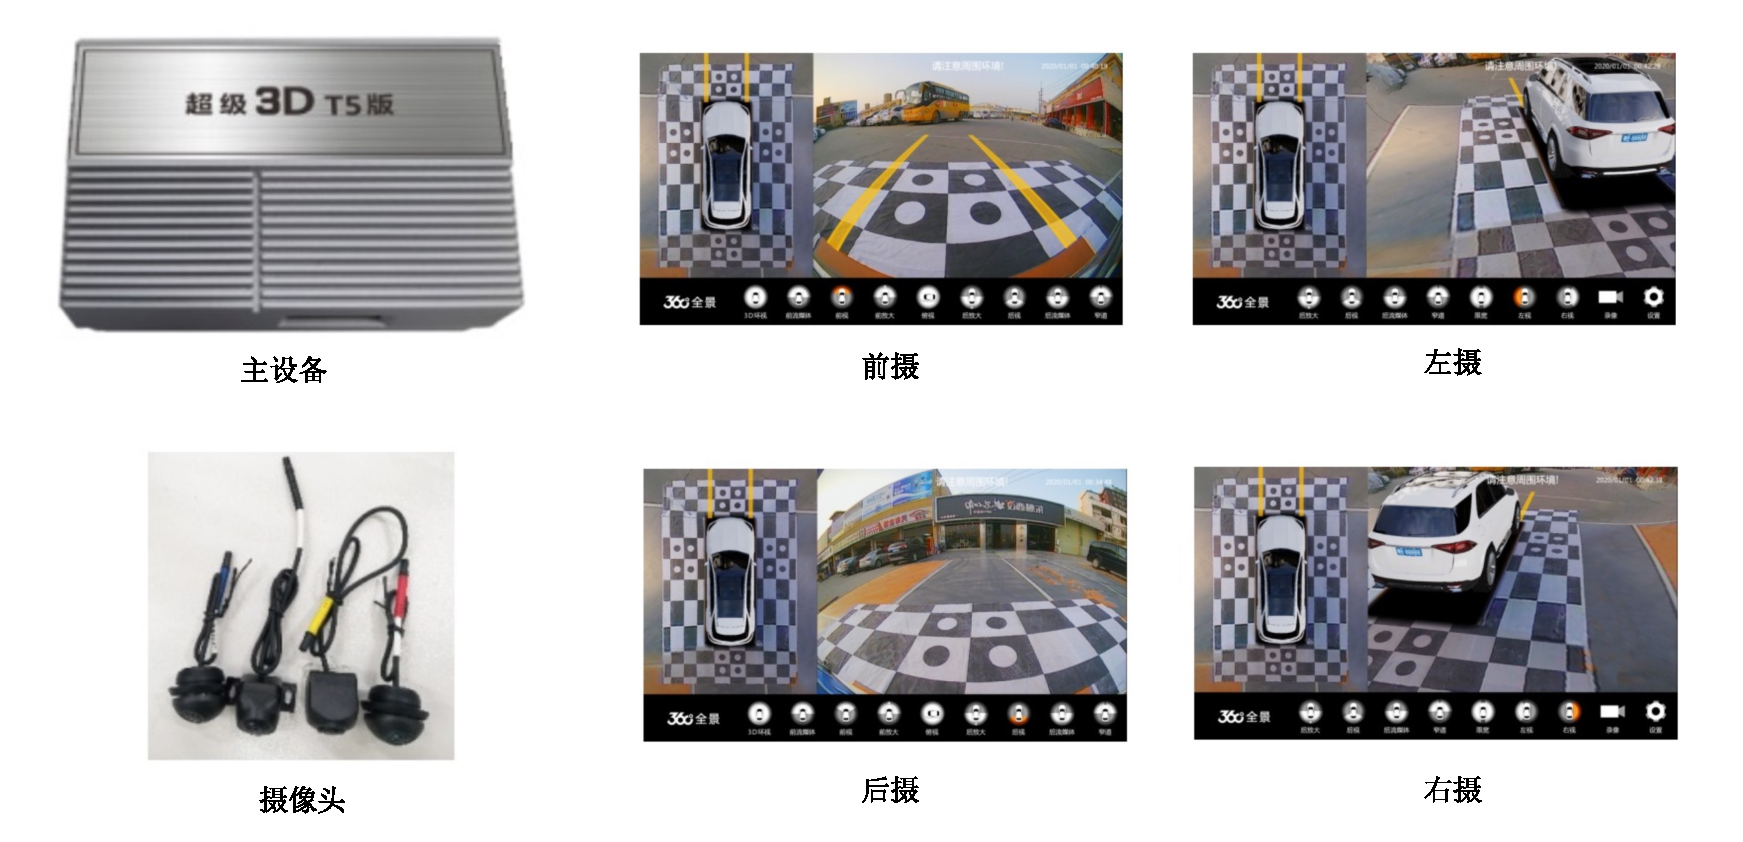
\includegraphics[width=1\textwidth]{figures/chp2/pdf/equip.pdf}
\caption{360度全景环视系统 \\Fig~\ref{fig_equip}~360-degree surround view system}
\label{fig_equip}
\end{figure}


\subsection{定量分析}
在本部分，本文通过深入的数据分析，展现 CRPS-D 数据集相较于现有数据集的显著改进与优势。

\begin{table}[!h]
\centering
\setlength{\tabcolsep}{4.0mm}
\caption{数据规模对比结果 \\Table~\ref{tab_datascale}~Comparison results of data scale}
\begin{tabular}{llccc}
        \toprule
         数据集  & & ps2.0\cite{zhang2018vision} & SNU\cite{do2020context} & \textbf{Ours} \\
        \midrule
             \multirow{3}{*}{总图像数} & 训练集 & 9827 & 18299 & 29803  \\
              & 测试集 & 2338 &	4518	&5936   \\
              & 总数 & 12165	& 22817	& \textbf{35739}  \\
        \midrule
            \multirow{3}{*}{训练集中的车位数}  & 垂直车位 & 9160 & 45610 & 103931  \\
              & 倾斜车位 & 316 &	3276 & 14126   \\
              & 总数 & 9476 & 48886 & \textbf{118057}  \\
        \midrule
             \multirow{3}{*}{测试集中的车位数}   & 垂直车位 & 2087 & 12541 & 21451 \\
              & 倾斜车位 & 81 & 1004 & 2573  \\
              & 总数 & 2168 & 13545 & \textbf{24024}   \\
        \midrule
             总车位数  & 总数 & 11644 & 62431 & \textbf{142081} \\
        \bottomrule
    \end{tabular}
\label{tab_datascale}
\end{table} 

（1）数据规模

数据集规模对于当下的视觉模型（如 SAM\cite{kirillov2023segment}）而言，重要性日益凸显，这也正是本文构建更大规模数据集的原因所在。在图像总数以及车位总数方面，CRPS - D 均实现了数量级的提升。如表\ref{tab_datascale}所示，CRPS-D 数据集的图像总数达 35739 张，分别为 ps2.0 和 SNU 的 2.94 倍与 1.57 倍。尤为突出的是，在总车位数量上，CRPS-D（142081 个）约为 ps2.0（11644 个）的 12.2 倍，为深度神经网络提供了高质量的学习样本。

此外，为进一步衡量数据集的丰富程度，本文计算了“车位-图像密度”（slot-image density），其表达式为：
\begin{equation}
 \mbox{车位图像密度} = \frac{N_{slots}}{N_{images}}
\end{equation}
其中，$N$ 表示不同条件下的样本数量。

在数据集丰富度的横向对比中，CRPS - D 展现出显著的统计优势。特别是其“车位-图像密度”高达 3.98，如表\ref{tab_density} 所示，远高于 ps2.0（0.96）和 SNU（2.74）。这一高密度特征表明，CRPS-D 能够为算法提供更为复杂的空间上下文以及重叠/遮挡样本，促使模型学习更为鲁棒的特征表示，而非简单的模板匹配。这为训练具备更高泛化能力的深度感知网络奠定了坚实的数据基础。 

\begin{table}[!h]
\centering
\caption{车位图像密度 \\Table~\ref{tab_density}~Density of parking slots }
\begin{tabular}{lccccccccc}
\toprule
 & \multicolumn{3}{c}{ps2.0\cite{zhang2018vision}} & \multicolumn{3}{c}{SNU\cite{do2020context}} & \multicolumn{3}{c}{\textbf{Ours}} \\\cmidrule{2-4}\cmidrule{5-7}\cmidrule{8-10}%
 
    & $N_{slots}$ &$N_{images}$ & 密度 & $N_{slots}$ &$N_{images}$ & 密度 & $N_{slots}$ &$N_{images}$ & 密度 \\
\midrule
     训练集 & 9476 & 9827 & 0.96 & 48886 & 18299 & 2.67 & 118057 & 29803 & \textbf{3.96}  \\
    测试集 & 2168 & 2338 & 0.93 & 13545 & 4518 & 3.00 & 24024 & 5936 & \textbf{4.05}  \\
    总数 & 11644 & 12165 & \textbf{0.96} & 62431 & 22817 & \textbf{2.74} & 142081 & 35739 & \textbf{3.98}  \\
\bottomrule
\end{tabular}
\label{tab_density}
\end{table} 



（2）场景分析

为全面覆盖现实世界中的复杂泊车环境，CRPS - D数据集细分为八个特定子集，涵盖“室内弱光 / 强光”、“室外日光 / 雨天 / 阴影 / 夜晚”以及“斜向车位”“受损车位”等多样化场景。如表\ref{tab_sence}所示，相较于基准数据集ps2.0，CRPS-D 在环境广度方面实现了显著突破。它不仅引入了更具挑战性的“室外夜晚”与“受损车位”场景，填补了现有数据集在极端场景下的空白，而且在各细分场景的图像数量级上均有大幅提升。

此外，为直观展现本数据集的优势，本文在图\ref{fig_crpsd}中展示了各场景的示例。从中能够观察到，CRPS-D比ps2.0更贴近现实情况。 


\begin{table}[!h]
\centering
\setlength{\tabcolsep}{1.0mm}
\caption{测试集场景统计信息\\
Table~\ref{tab_sence}~Statistics for the scene data in the test set.}
\begin{tabular}{lccccccccc}
    \toprule
    \multirow{2}{*}{场景} & \multicolumn{2}{c}{室内} & \multicolumn{4}{c}{室外} & \multicolumn{2}{c}{特殊场景} & \multirow{2}{*}{总计} \\
    \cmidrule(lr){2-3} \cmidrule(lr){4-7} \cmidrule(lr){8-9}
    & 弱光 & 强光 & 正常日光 & 雨天 & 阴影 & 夜晚 & 倾斜车位 & 受损车位 & \\
    \midrule
    ps2.0\cite{zhang2018vision} & \multicolumn{2}{c}{226} & 693 & 244 & 1127 & / & 48 & / & 2338 \\
    \textbf{Ours} & 545 & 786 & 1703 & 323 & 1389 & 86 & 802 & 302 & 5936 \\
    \bottomrule
\end{tabular}
\label{tab_sence}
\end{table}


\begin{figure}[!h]
\centering
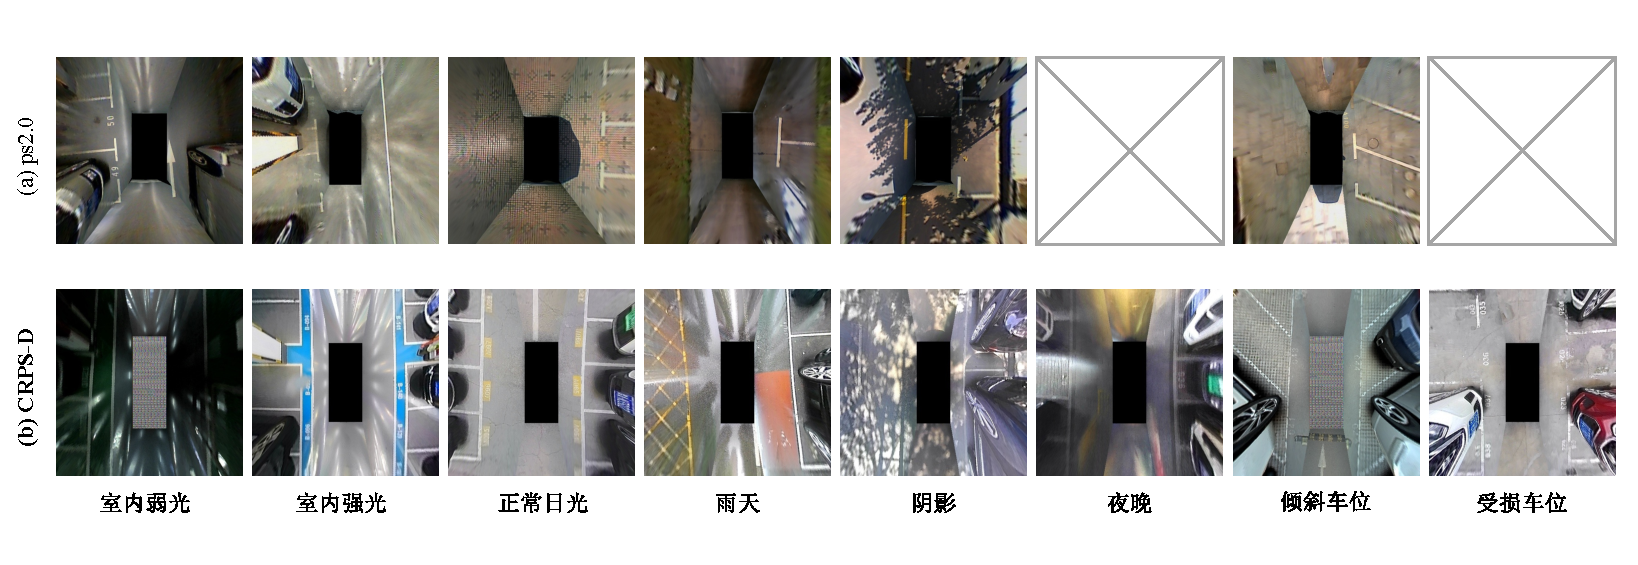
\includegraphics[width=1\textwidth]{figures/chp2/pdf/sence.pdf}
\caption{数据集示例图片 \\Fig~\ref{fig_crpsd}~Example images from the dataset}
\label{fig_crpsd}
\end{figure}

（3）倾斜车位

倾斜式停车位常应用于狭窄街道，旨在更有效地利用道路空间，在现实场景中较为常见。然而，相较于垂直式停车位，倾斜式停车位的检测难度更大，且常被其他数据集忽视。鉴于此，本文提高了倾斜式停车位在数据集中的比例。

倾斜式停车位在狭窄街道频繁使用，以提升道路空间利用率，是现实场景中常见的车位类型。但与垂直车位相比，倾斜车位检测难度更高，且常被其他数据集所忽略。因此，本文特意增加了倾斜车位在数据集中的占比。倾斜车位占比的计算公式如下：
\begin{equation}
 \mbox{倾斜车位比例} = \frac{S_{slant}}{S_{Total}}. 
\end{equation}
其中，$S$ 表示不同类型的停车位样本数量。

如表\ref{tab_slant}所示，本文的CRPS-D数据集包含11.75\%的斜向车位，这一比例显著高于ps2.0（3.41\%）和SNU（6.86\%）。这不仅更真实地反映了现实世界的实际情况，还有助于缓解类别不平衡问题。 

\begin{table}[!h]
\centering
\caption{倾斜停车位占比 \\
Table~\ref{tab_slant}~Proportion of slanted parking slots.}
\begin{tabular}{lccccccccc}
\toprule
 & \multicolumn{3}{c}{ps2.0\cite{zhang2018vision}} & \multicolumn{3}{c}{SNU\cite{do2020context}} & \multicolumn{3}{c}{\textbf{Ours}} \\\cmidrule{2-4}\cmidrule{5-7}\cmidrule{8-10}%
 
    & $S_{slant}$ &$S_{Total}$ & 占比 & $S_{slant}$ &$S_{Total}$ & 占比
    & $S_{slant}$ &$S_{Total}$ & 占比 \\
\midrule
    训练集 & 316 & 9476 & 3.33\% & 3276 & 48886 & 6.70\% & 14126 & 118057 & \textbf{11.97\%}  \\
    测试集 & 81 & 2168 & 3.74\% & 1004 & 13545 & 7.41\% & 2573 & 24024 & \textbf{10.71\%}  \\
    总数 & 397 & 11644 & \textbf{3.41\%} & 4280 & 62431 & \textbf{6.86\%} & 16699 & 142081 & \textbf{11.75\%}  \\
\bottomrule
\end{tabular}
\label{tab_slant}
\end{table} 




\section{半监督停车位检测算法框架}

在本节中，本文将详细阐述SS - PSD架构的构成以及所采用的半监督学习策略。如图\ref{fig_sspsd}所示，整个架构由两个分支构成：学习-学生分支，用于开展模型训练；以及指导-教师分支，在此分支中运用EMA（指数移动平均）以及$M_{\theta}^{S}$的参数来更新$M_{\theta}^{T}$。图中左下部分和右下部分分别对应\textbf{Adaptive - VAT}和\textbf{CGM Consistency}。 

\begin{figure}[!h]
\centering
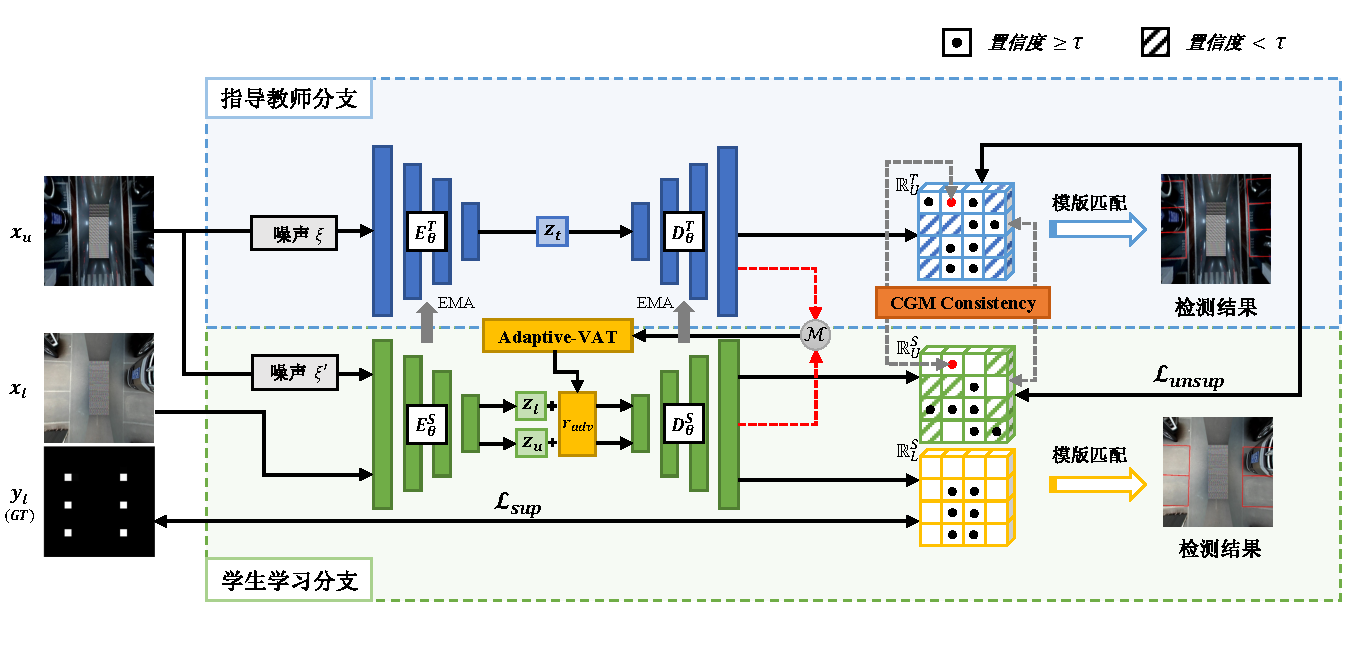
\includegraphics[width=1\textwidth]{figures/chp2/pdf/pipline.pdf}
\caption{SS-PSD的整体架构\\Fig~\ref{fig_sspsd}~Overview of SS-PSD architecture}
\label{fig_sspsd}
\end{figure}

\subsection{问题定义}

首先，本文随机选取一小部分带有对应标签的数据构成有标签数据集，记为\(\mathcal{D}_{L}=\{(\textbf{x}_{l},\textbf{y}_{l})\}\)，而剩余图像则构成无标签数据集\(\mathcal{D}_{U}=\{(\textbf{x}_{u})\}\)。给定一张尺寸为\(512\times512\)的图像\(\textbf{x}_{l}\)及其对应标签\(\textbf{y}_{l}\)，本研究旨在预测一个特征图\(\mathbb{R} \in \mathcal{S}\times \mathcal{S} \times \mathcal{N}\)，其中图像被划分为\(\mathcal{S}\times \mathcal{S}\)个网格。参照DMPR - PS~\cite{huang2019dmpr}的方法，特征图\(\mathbb{R}\)与输入图像中的标线点相对应，\(\mathcal{N}\)个维度代表它们各自的特征。随后，本文应用模板匹配来判定这些点能否构成有效的入口线，进而识别出相应的车位。这一过程可描述如下：

\begin{equation}
\textbf{x}_{l} \xrightarrow{M_{\theta}} \mathbb{R}^{\mathcal{S}\times \mathcal{S} \times \mathcal{N}} \xrightarrow {\text{模版匹配}} \text{停车检测结果}
\end{equation}

其中\(M_{\theta}(\cdot)\)是用于预测标记点的模型，\(\theta\)代表模型参数。
与以往过度依赖昂贵有标签数据集的研究不同，本文利用易于获取的无标签图像\(\textbf{x}_{u}\)来进一步提升性能。 

\subsection{网络架构}

图\ref{fig_sspsd}展示了本文所提出的半监督停车位检测基线模型 (SS - PSD) 的架构，该模型由一个指导教师分支和一个学习学生分支构成。二者具有相同的网络结构，记为\(M_{\theta}=\{E_{\theta}, D_{\theta}\}\)，其中包含编码器\(E_{\theta}: \textbf{x}\rightarrow \textbf{z}\)和解码器\(D_{\theta}: \textbf{z}\rightarrow \mathbb{R}^{\mathcal{S} \times \mathcal{S} \times \mathcal{N}}\)。
具体来讲，本文将教师模型定义为\(M_{\theta}^{T}=\{E_{\theta}^{T}, D_{\theta}^{T}\}\)，学生模型定义为\(M_{\theta}^{S}=\{E_{\theta}^{S}, D_{\theta}^{S}\}\)。

（1）学生分支

本文采用定制的CNN模型~\cite{huang2019dmpr}作为编码器-解码器架构。在学习-学生分支中，编码器\(E_{\theta}^{S}\)同时处理已标注的\(\textbf{x}_{l}\)和未标注的\(\textbf{x}_{u}\)数据，生成潜在特征\(\textbf{z}_{l}\)和\(\textbf{z}_{u}\)，可表示为\(E_{\theta}^{S}(\textbf{x}_{l} / \textbf{x}_{u}) = \textbf{z}_{l} / \textbf{z}_{u}\)。
结合自适应VAT算法生成的对抗噪声\(\textbf{r}_{adv}\)，将\(\textbf{z}_{u}\)和\(\textbf{z}_{l}\)输入解码器\(D_{\theta}^{S}\)，生成最终特征图，可表示为\(D_{\theta}^{S}(\textbf{z}_{l} / \textbf{z}_{u} + \textbf{r}_{adv}) = \mathbb{R}_{L}^{S} / \mathbb{R}_{U}^{S}\)。
所得特征图\(\mathbb{R}\)对应于输入图像中的标记点。随后，本文采用模板匹配方法系统地验证几何关系，判断这些点是否排列成有效的停车位入口线。

（2）教师分支

在此分支中，未标记数据\(\textbf{x}_{u}\)经\(E_{\theta}^{T}\)处理，生成潜在特征\(\textbf{z}_{t}\)，表示为\(E_{\theta}^{T}(\textbf{x}_{u}) = \textbf{z}_{t}\)。然后，该潜在特征被输入到\(D_{\theta}^{T}\)中，生成最终特征图\(\mathbb{R}_{U}^{T}\)，表示为\(D_{\theta}^{T}(\textbf{z}_{t}) = \mathbb{R}_{U}^{T}\)。在训练过程中，本文采用自适应矩估计（Adam）~\cite{kingma2014adam}来最小化\(M_{\theta}^{S}\)的损失函数，同时使用EMA~\cite{tarvainen2017mean}和\(M_{\theta}^{S}\)的参数来更新\(M_{\theta}^{T}\)。 


\subsection{自适应特征扰动}
特征扰动是自监督或半监督学习中广泛采用的策略。在本研究中，并未引入随机噪声，而是借助虚拟对抗训练（VAT\cite{miyato2018virtual}）来估计对抗噪声。该噪声旨在使扰动后预测与原始预测之间的距离最大化。如图\ref{fig_sspsd}左下部分所示，给定分离的潜在特征\(\textbf{z}\)，通过计算梯度引导的对抗噪声\(\textbf{r}\)，让\((D_\theta(\textbf{z}+\textbf{r}) - D_\theta(\textbf{z}))\)达到最大，以此尽可能干扰网络。要达到理想的扰动效果，\(D_\theta\)的模型质量至关重要，因其决定了梯度的搜索方向。

Liu等人\cite{liu2022perturbed}在PS-MT中提出了T-VAT方法，该方法设定\(D_\theta\)为教师模型\(D_{\theta}^{T}\)来计算对抗噪声。但本文认为，这一设定并非总是最优。通过实验观察发现，在特定情形下（尤其是训练初期），学生模型\(D_{\theta}^{S}\)由于受到直接梯度引导，往往表现出更好的特征质量。因此，本文引入了自适应虚拟对抗训练（Adaptive - VAT），以施加最优扰动。该机制依据教师模型和学生模型在生成扰动时的抗扰鲁棒性，自适应地从二者中选择最优的对抗噪声。

具体来讲，Adaptive - VAT不再盲目信赖教师模型生成的扰动方向，而是通过实时评估学生模型与教师模型的确定性强度，动态构建更具挑战性的负样本，如图\ref{fig_sspsd}左下部分所示。这种竞争机制促使学生模型在更为严苛的特征空间内学习稳健的车位几何表征。
为确保原始预测与扰动后预测之间的距离最大化，对抗噪声\(\textbf{r}_{adv}\)综合参考\(D_{\theta}^{T}\)和\(D_{\theta}^{S}\)的响应进行计算，且需满足以下公式：
\begin{equation}
\begin{align}
\text{maximise }& \mathcal{M}\Big(d(D_{\theta}^{T}(\mathbf{z}_l / \mathbf{z}_u) , D_{\theta}^{T}(\mathbf{z}_l / \mathbf{z}_u + \textbf{r}_{adv})), 
&d(D_{\theta}^{S}(\mathbf{z}_l / \mathbf{z}_u), D_{\theta}^{S}(\mathbf{z}_l / \mathbf{z}_u + \textbf{r}_{adv}))
\Big),\\
\text{subject to }& ||\mathbf{r}_{adv}||_2 <=\epsilon,
\end{align}
\end{equation}
其中 $d(\cdot,\cdot)$ 表示均方误差 (MSE) 损失，$\mathcal{M}(\cdot,\cdot)$ 选择 MSE 损失更低的更优解码器。

\subsection{一致性约束}
为构建针对无标签数据的一致性约束，一个直观思路是计算学生模型预测结果\(\mathbb{R}_{U}^{S}\)与教师模型预测结果\(\mathbb{R}_{U}^{T}\)之间的均方误差（MSE\cite{tarvainen2017mean}）损失，以此确保预测的一致性。然而，此方案可能致使潜在的错误预测也被强制保持一致，进而误导网络学习；并且，对特征图\(\mathbb{R}\)中所有网格单元赋予均等权重也并非最优选择。
针对该问题，如图\ref{fig_sspsd}右下部分所示，本文引入置信度图（Confidence Map），为不同的网格单元分配非均衡的注意力，并对低置信度区域进行 Mask。

具体而言，对于特征图\(\mathbb{R} \in \mathcal{S} \times \mathcal{S} \times \mathcal{N}\)，本文将输入图像\(\textbf{x}\)划分为\(16×16\)的网格（即\(\mathcal{S} = 16\)），并设定特征维度\(\mathcal{N} = 9\)（即\(6 + 3\)）。其中，前6个维度遵循DMPR - PS~\cite{huang2019dmpr}的设定，而新增的3个维度用于捕捉检测斜向车位所需的角度及分类细节。也就是说，一个标线点的表征由9个分量构成：用于基准点定位的\((x, y)\)、用于两条边缘角度的\((\cos\theta_{1/2}, \sin\theta_{1/2})\)、标线点形状\(\textbf{s}\)、标线点类型\(\textbf{t}\)（即垂直或斜向）以及置信度\(C\)。

因此，本文最终构建了置信度引导的掩码一致性损失\(\mathcal{L}_{CGM}\)，其表达式为：
\begin{equation}
\begin{cases}
\sum_{i=1}^{\mathcal{S}^{2}} \{ ||C_{i}^{S} - C_{i}^{T}||_2 \} & \text{if } C_{i}^{T} < \tau \\
\sum_{i=1}^{\mathcal{S}^{2}} \{ ||C_{i}^{S} - C_{i}^{T}||_2 + ||q_{i}^{S} - q_{i}^{T}||_2 \times C_{i}^{T} \} & \text{if } C_{i}^{T} \geq \tau
\end{cases}
,
\end{equation}

其中\(q = (x,y,\cos\theta_1,\sin\theta_1,\cos\theta_2,\sin\theta_2,\textbf{s},\textbf{t})\)，下标\(i\)表示\(16×16\)网格中的单元格索引，\(\tau\)为置信阈值（本文设定\(\tau = 0.9\)）。如此一来，本文不仅能够筛选出重要的网格单元格进行监督，还能更加聚焦于那些更有可能包含标记点的网格单元格。 


\subsection{损失函数}
（1）标注数据

对于已标注的图像对 $(\textbf{x}_{l},\textbf{y}_{l})$，可以为预测提供直接的监督。因此，监督损失 $\mathcal{L}_{sup}$ 定义如下：

\begin{equation}
\begin{cases}
\sum_{i=1}^{\mathcal{S}^{2}} \{ ||C_{i}^{S}||_2 \} & \text{if } \textbf{y}_{li} \ 不存在 \\
\sum_{i=1}^{\mathcal{S}^{2}} \{ ||C_{i}^{S} - 1||_2 + ||q_{i}^{S} - \hat{q_{i}}||_2 \} & \text{if } \textbf{y}_{li} 存在
\end{cases}
,
\end{equation}%

其中 $\hat{q_{i}}$ 表示对应的真实值。对于预测而言，(GT) 函数 $\textbf{y}_{li}$ 仅当标记点位于网格单元 $i$ 内时才存在。

（2）未标注数据

对于未标记数据，本文利用 $M_{\theta}^{T}$ 和 $M_{\theta}^{S}$ 之间的置信度引导掩码 (CGM) 一致性来建立无监督约束，如下式所示：

\begin{equation}
\mathcal{L}_{unsup}(\mathcal{D}_{U}, M_{\theta}^{S}, M_{\theta}^{T})=\mathcal{L}_{CGM}
\end{equation}

总目标函数由基于标记数据和未标记数据的两项组成，如下所示：

\begin{equation}
\begin{array}{l}
\mathcal{L}_{total}(\mathcal{D}_{L},\mathcal{D}_{U}, M_{\theta}^{S}, M_{\theta}^{T})= 
\mathcal{L}_{sup}(\mathcal{D}_{L}, M_{\theta}^{S})+ \beta \mathcal{L}_{unsup}(\mathcal{D}_{U}, M_{\theta}^{S}, M_{\theta}^{T})
\end{array}
,
\end{equation}

其中 $\beta=\frac{N_{\mathcal{D}_{U}}}{N_{\mathcal{D}_{L}}}$ 和 $N_{\mathcal{D}_{U}}/N_{\mathcal{D}_{L}}$ 分别表示标记样本和未标记样本的数量。

\section{实验结果及分析}
本节所有实验均在同一硬件平台上进行，具体包括一块 Nvidia 2080Ti GPU（12GB 显存）和一台配备 Intel(R) Xeon(R) E5-2680 v4 @ 2.40GHz 的 CPU 的服务器环境。模型训练使用 PyTorch 框架实现。

\subsection{不同数据划分的结果}

参照Mean Teacher\cite{tarvainen2017mean}方法，本节通过对数据集进行比例抽样来评估所提方法，其中有标签集的比例为\(1/n\)，无标签集的比例为\((1 - \frac{1}{n})\)。针对本文提出的CRPS-D数据集以及公开数据集ps2.0，分别采用\(1/24\)、\(1/12\)、\(1/8\)、\(1/4\)和\(1/2\)的有标签比例进行实验。鉴于本文的SS-PSD是该领域首个半监督解决方案，因此仅能将该方法与现有的公开全监督方案作对比。

（1）CRPS-D

如表\ref{tab_crpsd}所示，在标注比例为\(1/24\)（即1242张标注图像）的情形下，本文方法在\(AP_{parking - slot}\)上相较于DMPR - PS~\cite{huang2019dmpr}和GCN~\cite{min2021attentional}分别提升了\(19.02\%\)和\(16.49\%\)。即便在其他标注比例（\(1/12\)、\(1/8\)和\(1/4\)）下，本文方法也始终能实现\(6\%\)到\(12\%\)的性能提升。这些结果表明，本文方法能够有效利用未标注数据，进而获得显著的性能提升。标有\( * \)的表示经过重新训练的方法。

\begin{table}[!h]
\centering
\caption{不同标注比例下与开源SoTA方法对比（CPPS-D）\\
Table~\ref{tab_crpsd}~Comparison with open-source SoTA methods under different label ratios (CPPS-D)}
\begin{tabular}{lcccccc}
\toprule
Ratio & 1/24 & 1/12 & 1/8  & 1/4  & 1/2  & 1/1 \\
\midrule
  标签数 & 1242  & 2484  & 3726 & 7452  & 14901  & 29803  \\
  图片数 & 29803  & 29803  & 29803  & 29803  & 29803 & 29803 \\
\midrule
DMPR-PS$^{*}$\cite{huang2019dmpr}  & 52.70\% & 66.84\% & 70.28\% & 76.98\% & 83.23\% & 87.20\% \\
GCN$^{*}$\cite{min2021attentional}   & 55.23\% & 63.32\% & 67.80\% & 72.57\% & 76.31\% & 79.44\% \\
\textbf{Ours} & \textbf{71.72\%} & \textbf{79.75\%} & \textbf{81.03\%} & \textbf{83.78\%}  & \textbf{86.51\%} & \textbf{/} \\
\bottomrule
\end{tabular}
\label{tab_crpsd}
\end{table}

(2)ps2.0

本文还在ps2.0数据集上展开测试，以验证所提方法在不同停车位数据集上的泛化能力。表\ref{tab_ps2}显示，本文模型在所有分区协议下均优于监督式基线模型。

\begin{table}[!h]
\centering
\caption{不同标注比例下与开源SoTA方法对比（ps2.0）\\
Table~\ref{tab_ps2}~Comparison with open-source SoTA methods under different label ratios (ps2.0)}
\begin{tabular}{lcccccc}
\toprule
Ratio & 1/24 & 1/12 & 1/8  & 1/4  & 1/2  & 1/1 \\
\midrule
  标签数 & 410  & 819  & 1230 & 2457  & 4913  & 9827  \\
  图片数 & 9827  & 9827  & 9827  & 9827  & 9827  & 9827  \\
\midrule
    DMPR-PS$^{*}$\cite{huang2019dmpr}  & 60.95\% & 78.05\% & 87.28\% & 93.70\% & 96.47\% & 98.64\% \\
    GCN$^{*}$\cite{min2021attentional}  & 76.70\% & 85.72\% & 92.78\% & 95.47\% & 97.45\% & 98.31\% \\
    \textbf{Ours} & \textbf{80.44\%} & \textbf{90.47\%} & \textbf{94.52\%}  & \textbf{96.10\%} & \textbf{97.79\%} & \textbf{/} \\
\bottomrule
\end{tabular}
\label{tab_ps2}
\end{table}


\begin{figure}[!h]
    \centering
	  \subfloat[CRPS-D]{
       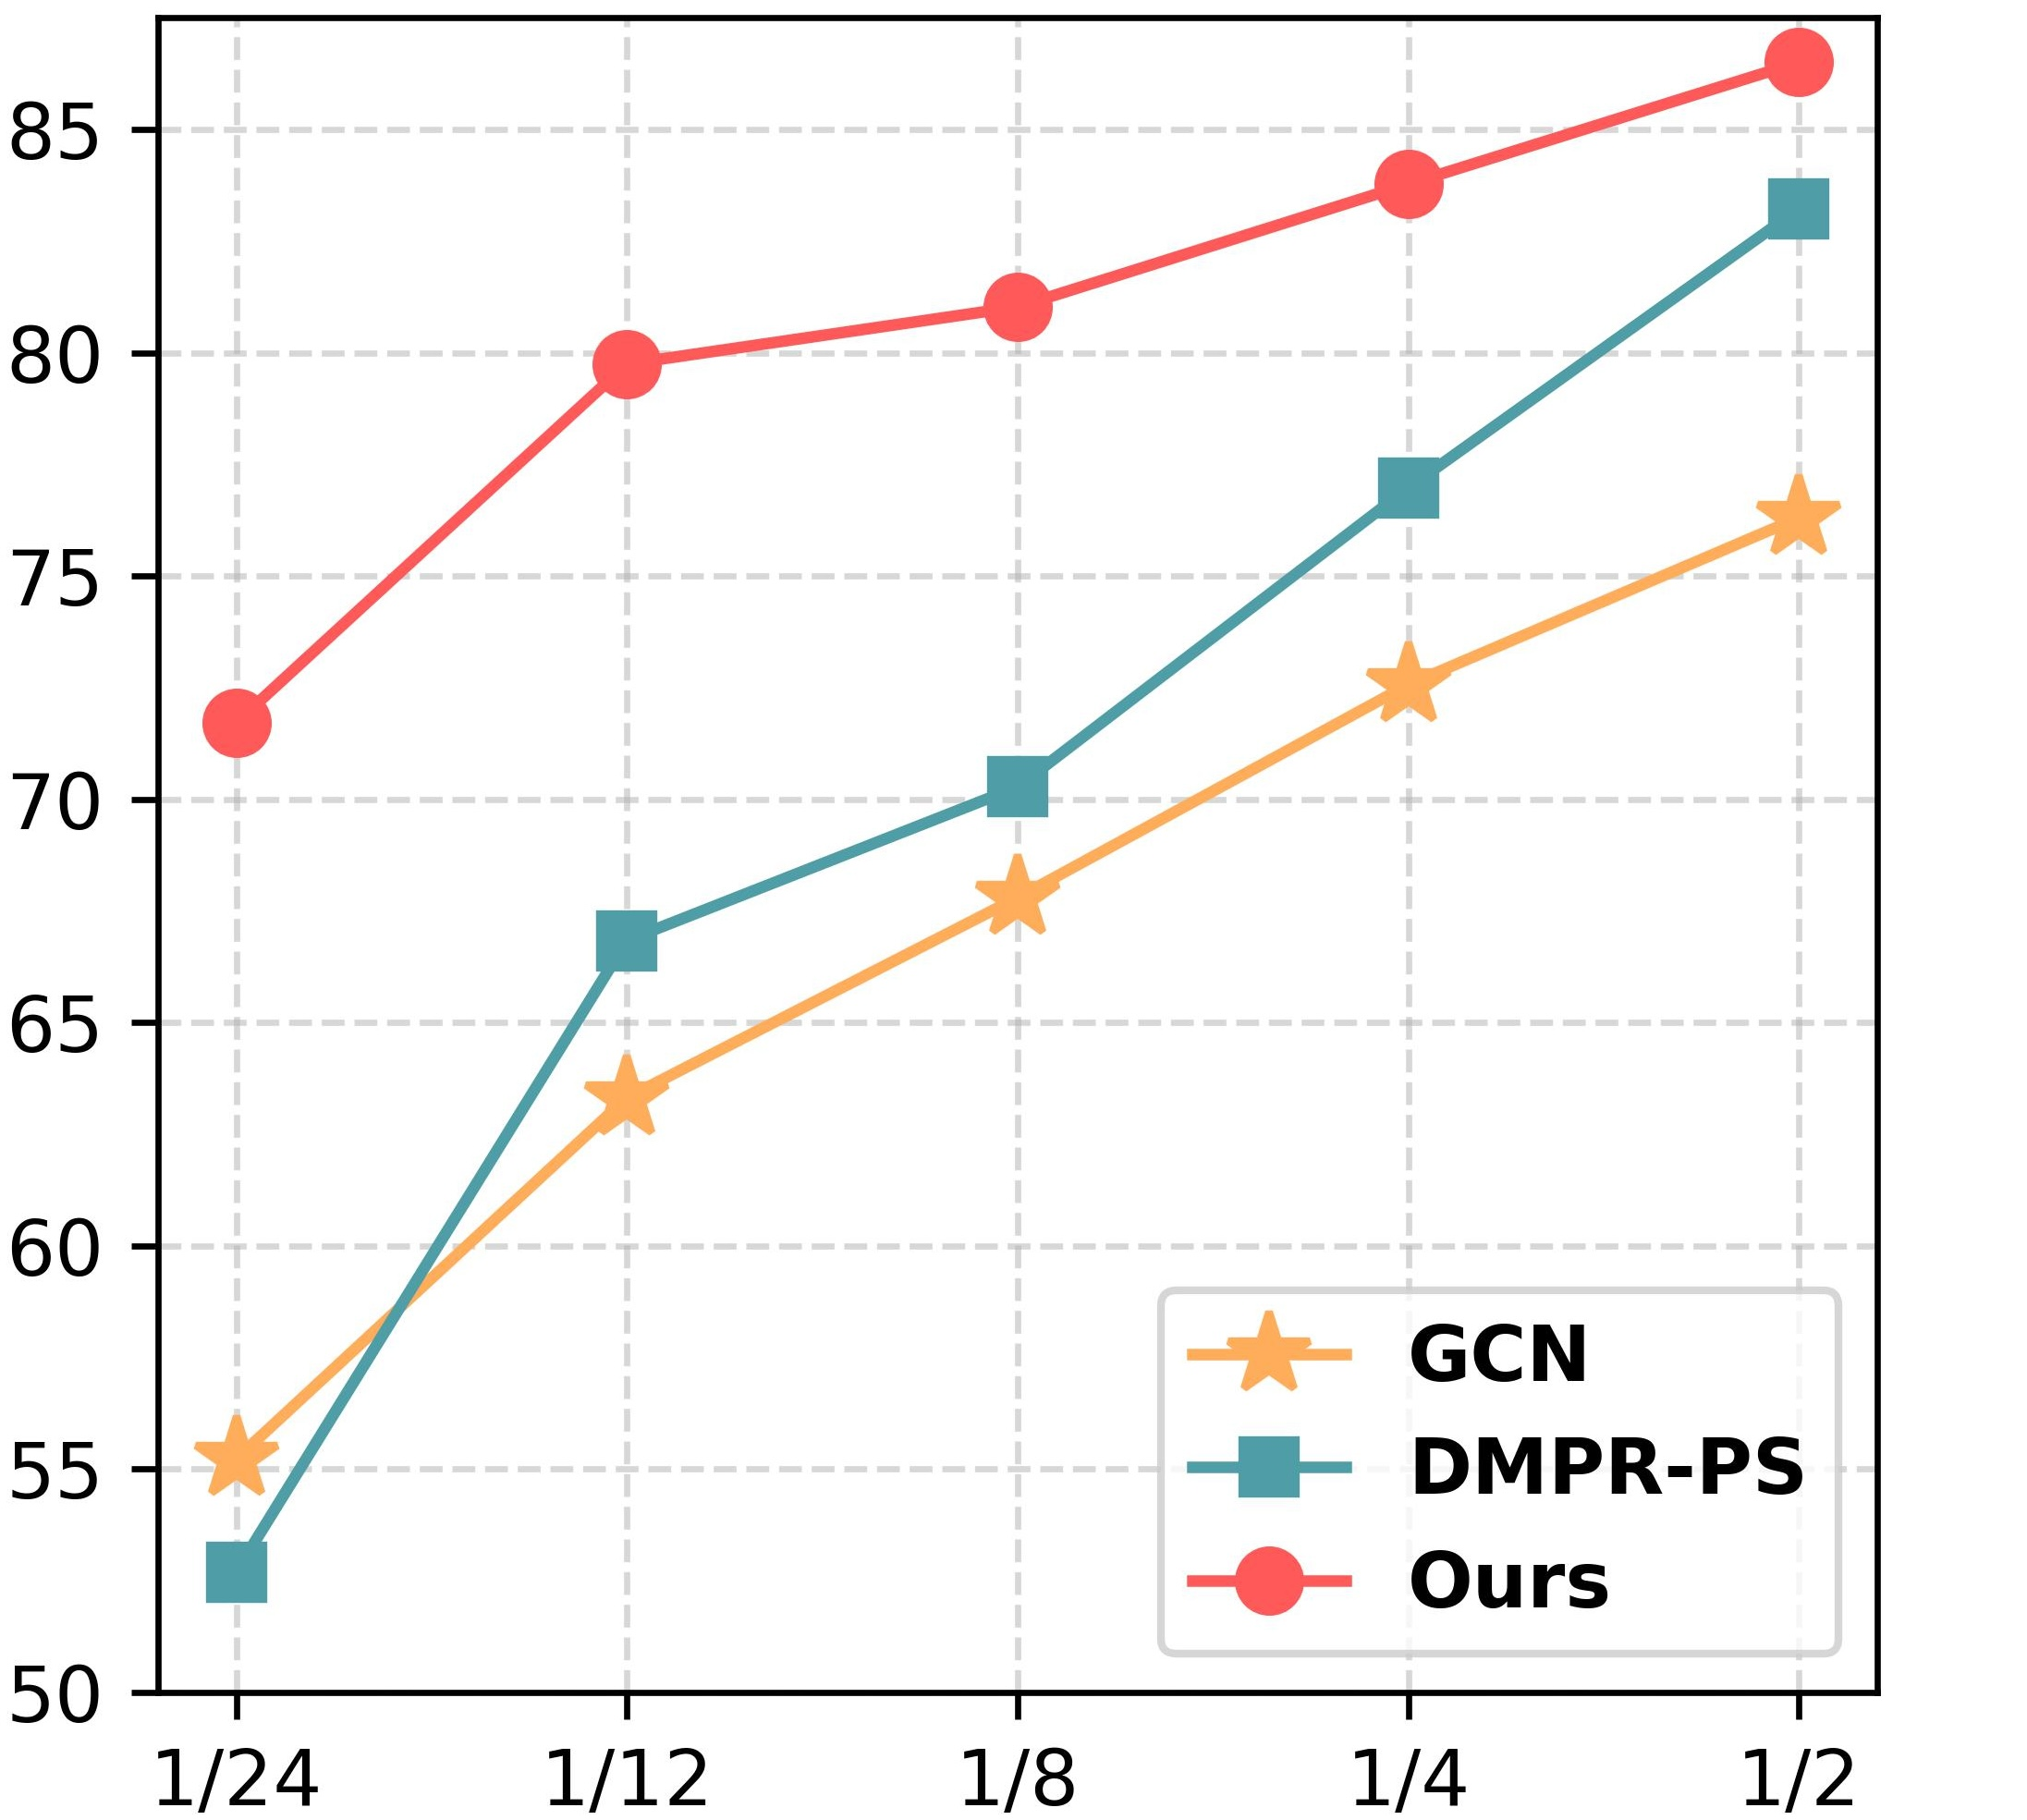
\includegraphics[width=0.43\linewidth]{figures/chp2/curve/curve_s2.jpg}}
    \label{5a}
	  \subfloat[ps2.0]{
        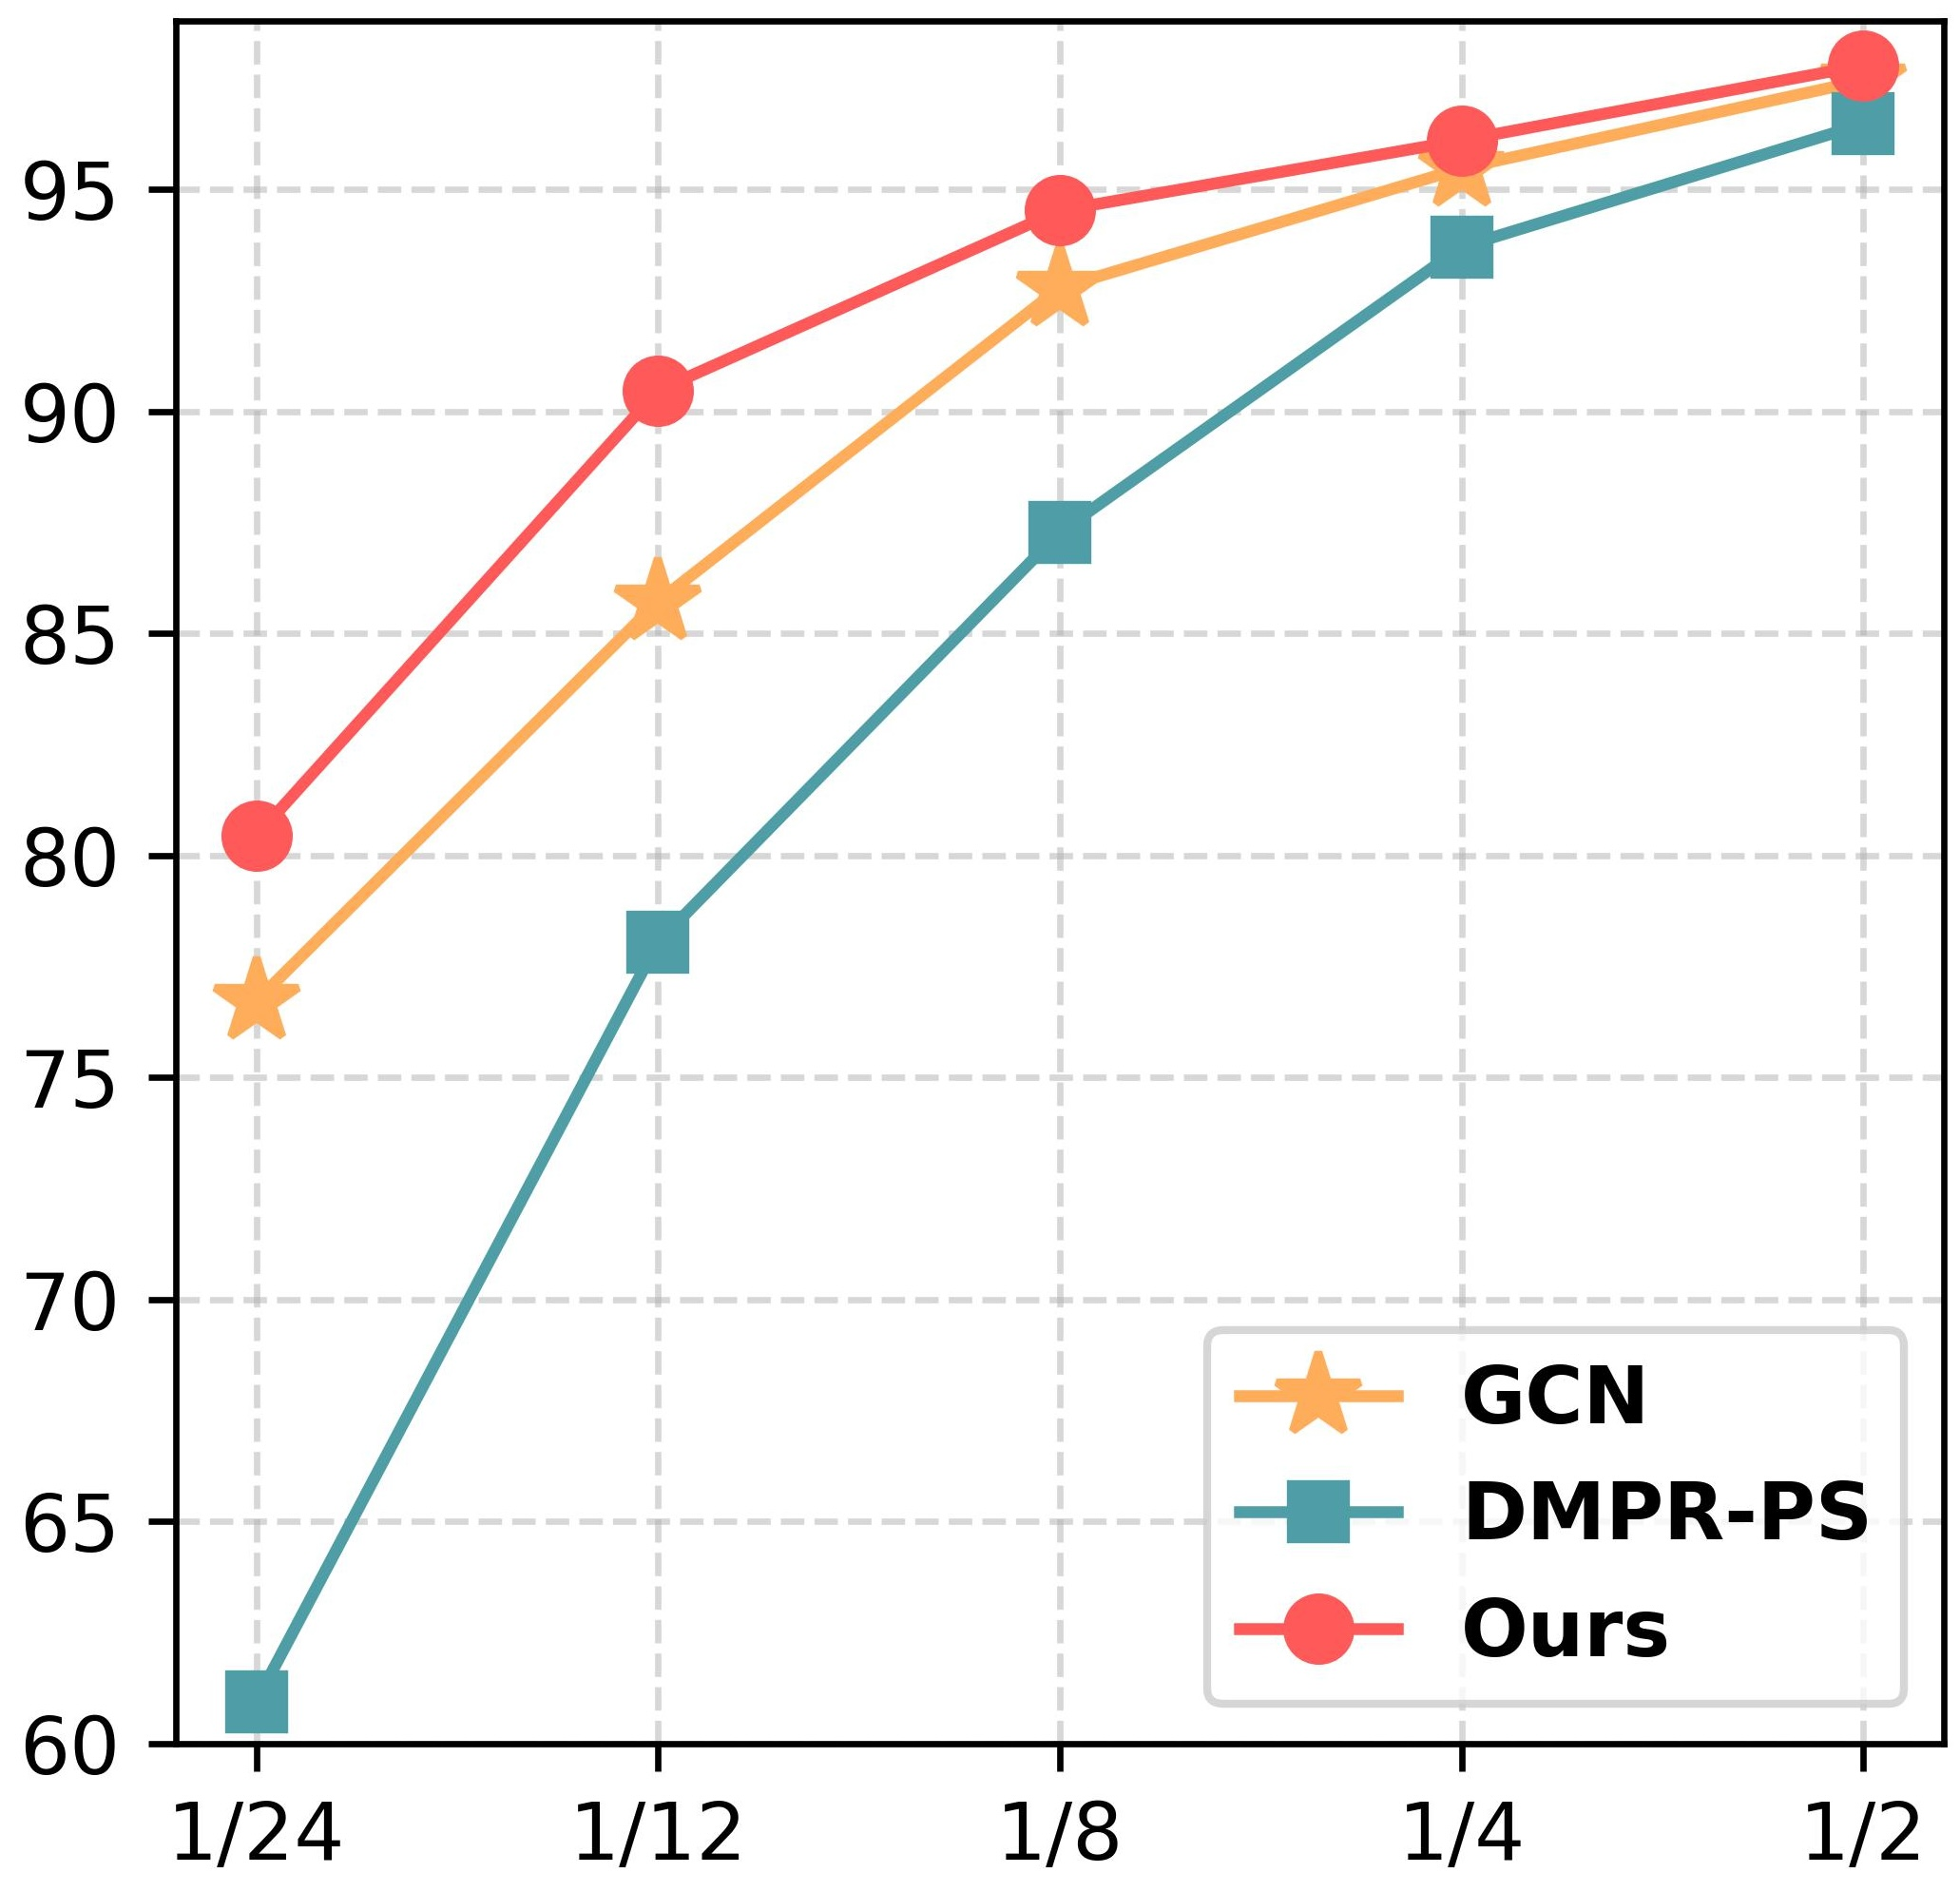
\includegraphics[width=0.4\linewidth]{figures/chp2/curve/curve_s1.jpg}}
    \label{5b}
    \caption{与监督基线相比的改进情况 \\Fig~\ref{fig_curve}~ Improvements over the supervised baseline}
    \label{fig_curve} 
\end{figure}

图\ref{fig_curve}展示了本文方法和监督基线在(a) CRPS-D 和(b) ps2.0上采用不同分区协议的结果。由于CRPS-D数据集相较于ps2.0数据集具有更高的复杂性与真实性，因此本文模型在CRPS-D数据集上相较于监督式基线模型的表现提升更为显著，特别是在标注数据量较少的情况下。所提出的半监督方法能够有效地从CRPS-D数据集中提取更为广泛的特征。 


\subsection{未标记数据有效性分析}

需要说明的是，本文首次提出用于停车位检测的半监督方法，因此直接将其与全监督方法作比较并非完全公平。

\begin{table}[ht]
\centering
\setlength{\tabcolsep}{3mm}
\caption{与近期方法的比较结果 \\
Table~\ref{tab_recent}~Comparison results with recent methods.}
\begin{tabular}{lccccc}
\toprule
    方法 & 标签数 & 图像数 &  Precision & Recall & F1 \\
\midrule
    SAM-PS\cite{zhai2024sam} & 0 & 9827 & 94.29\% & 81.35\% & 87.34\% \\
    \textbf{Ours (1/12)} & \textbf{819} & 9827 & \textbf{95.45\%} & \textbf{91.30\%} & \textbf{93.34\%} \\
\midrule
       DeepPS\cite{zhang2018vision}  & 9827 & 9827 & 98.99\% & 99.13\% & 99.06\% \\
       DMPR-PS\cite{huang2019dmpr} & 9827 & 9827 & 99.42\% & 99.37\% & 99.39\% \\
       VPS\cite{li2020vacant}  & 9827 & 9827 & 99.63\% & 99.10\% & 99.36\% \\
       GCN\cite{min2021attentional}  & 9827 & 9827 & 99.56\% & 99.42\% & 99.49\%\\
       SCCN \cite{zheng2022center}  & 9827 & 9827 & 99.35\% & 99.17\% & 99.26\% \\
       Bui et al.\cite{bui2023one} & 9827 & 9827 &  99.63\% & 99.63\% & 99.63\% \\
       BEV-PolyNet\cite{duan2025bev} & 9827 & 9827 &  99.82\% & 99.65\% & 99.73\% \\
       \textbf{Ours (1/2)} & \textbf{4913}  & 9827 & 98.64\% & 98.07\% & 98.35\%\\
\bottomrule
\end{tabular}
\label{tab_recent}
\end{table}

即便如此，本文仍提供更多与近期方法的对比结果。需注意，这些方法（如SCCN(2020)\cite{zheng2022center}、Bui等人(2023)\cite{bui2023one} 以及SAM - PS(2024)\cite{zhai2024sam}）并非开源，所以本文只能报告其原始论文在ps2.0数据集上的性能。结果如表 \ref{tab_recent} 所示，其中“Ours (1/n)”表示使用\(1/n\)个标签进行训练。

当仅使用\(1/12\)的标签（819个）时，本文的半监督方法性能显著优于现有的自监督方法（SAM-PS\cite{zhai2024sam}）。此外，当使用一半的标签（4913个）时，本文方法获得了与全监督模型（如VPS\cite{li2020vacant}）相当的性能，差异仅约为\(1\%\)。

此外，本节还展示了随着标注数据比例增加，SS-PSD与完全监督模型（本文的基线模型DMPR-PS \cite{huang2019dmpr}）之间的性能差距。如图 \ref{fig_ps} 和 \ref{fig_crps} 所示，当仅有少量标注数据时，SS-PSD的性能始终优于完全监督基线模型。黄色部分表示SS-PSD方法带来的性能提升，随着标注数据量增多，这种性能差距逐渐缩小。这种收益递减现象符合预期，因为一旦有足够的标注数据，利用未标注数据的边际收益便会降低。

    \begin{figure}[!h]
    \centering
    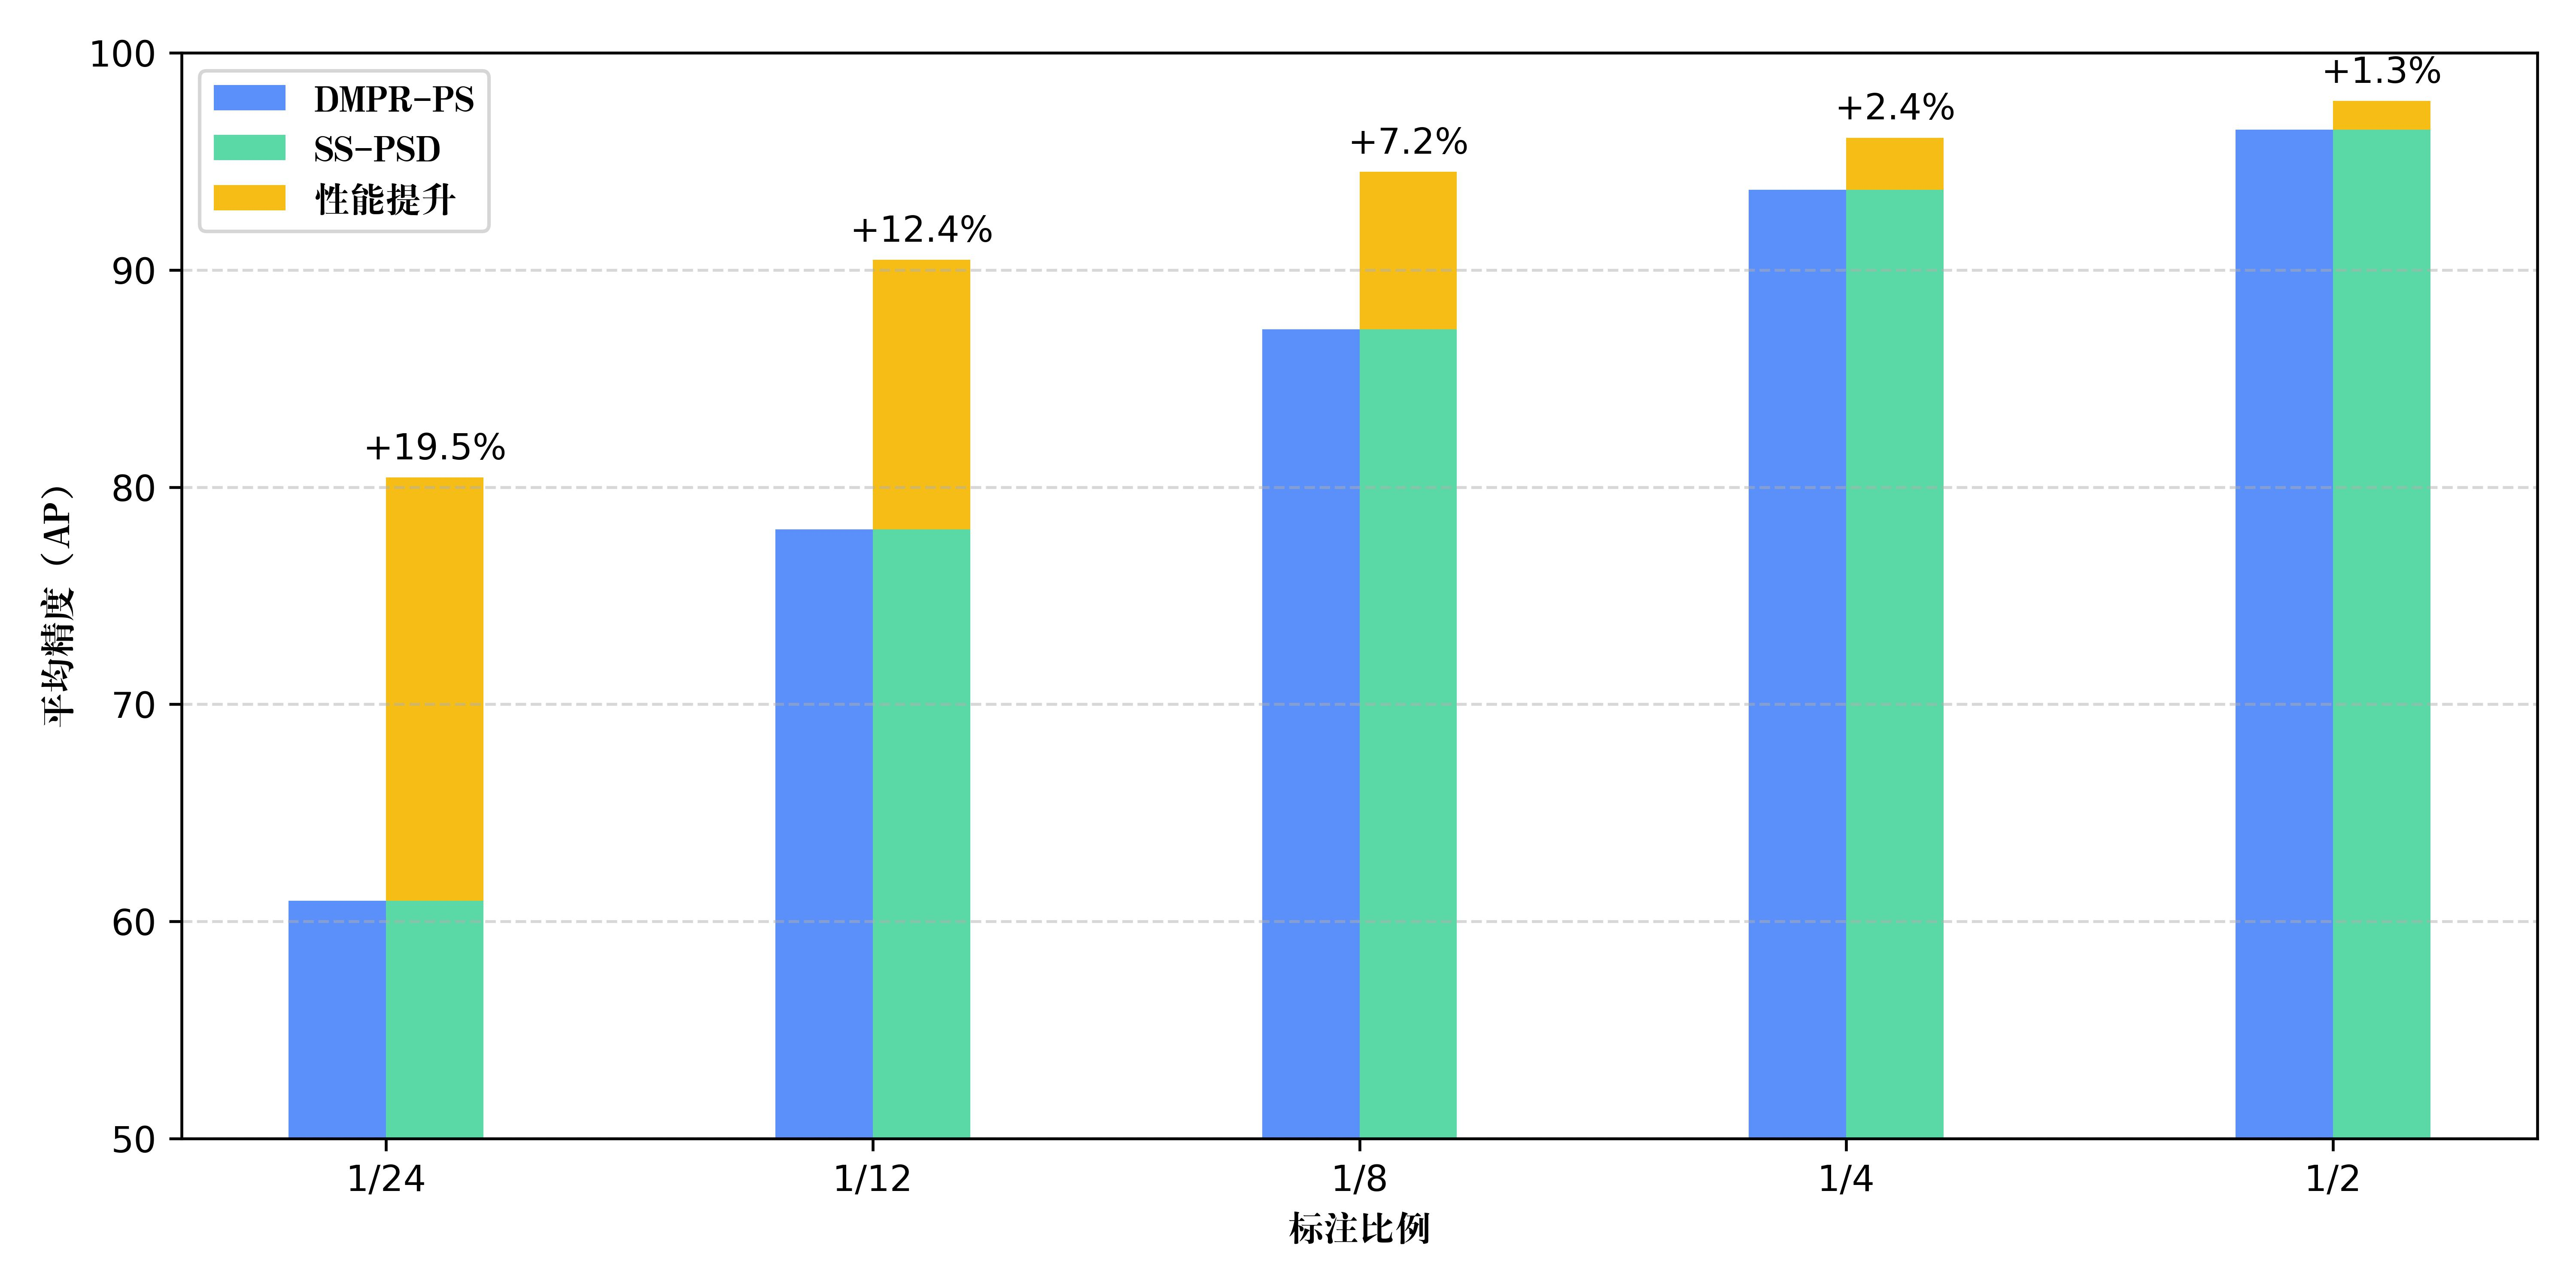
\includegraphics[width=1\linewidth]{figures/chp2/bar/ps.jpg}
    \caption{SS-PSD与DMPR-PS的性能比较（ps2.0数据集） \\Fig~\ref{fig_ps}~ Performance comparison of SS-PSD and DMPR-PS (ps2.0 dataset)}
    \label{fig_ps}
   \end{figure}

    \begin{figure}[!h]
    \centering
    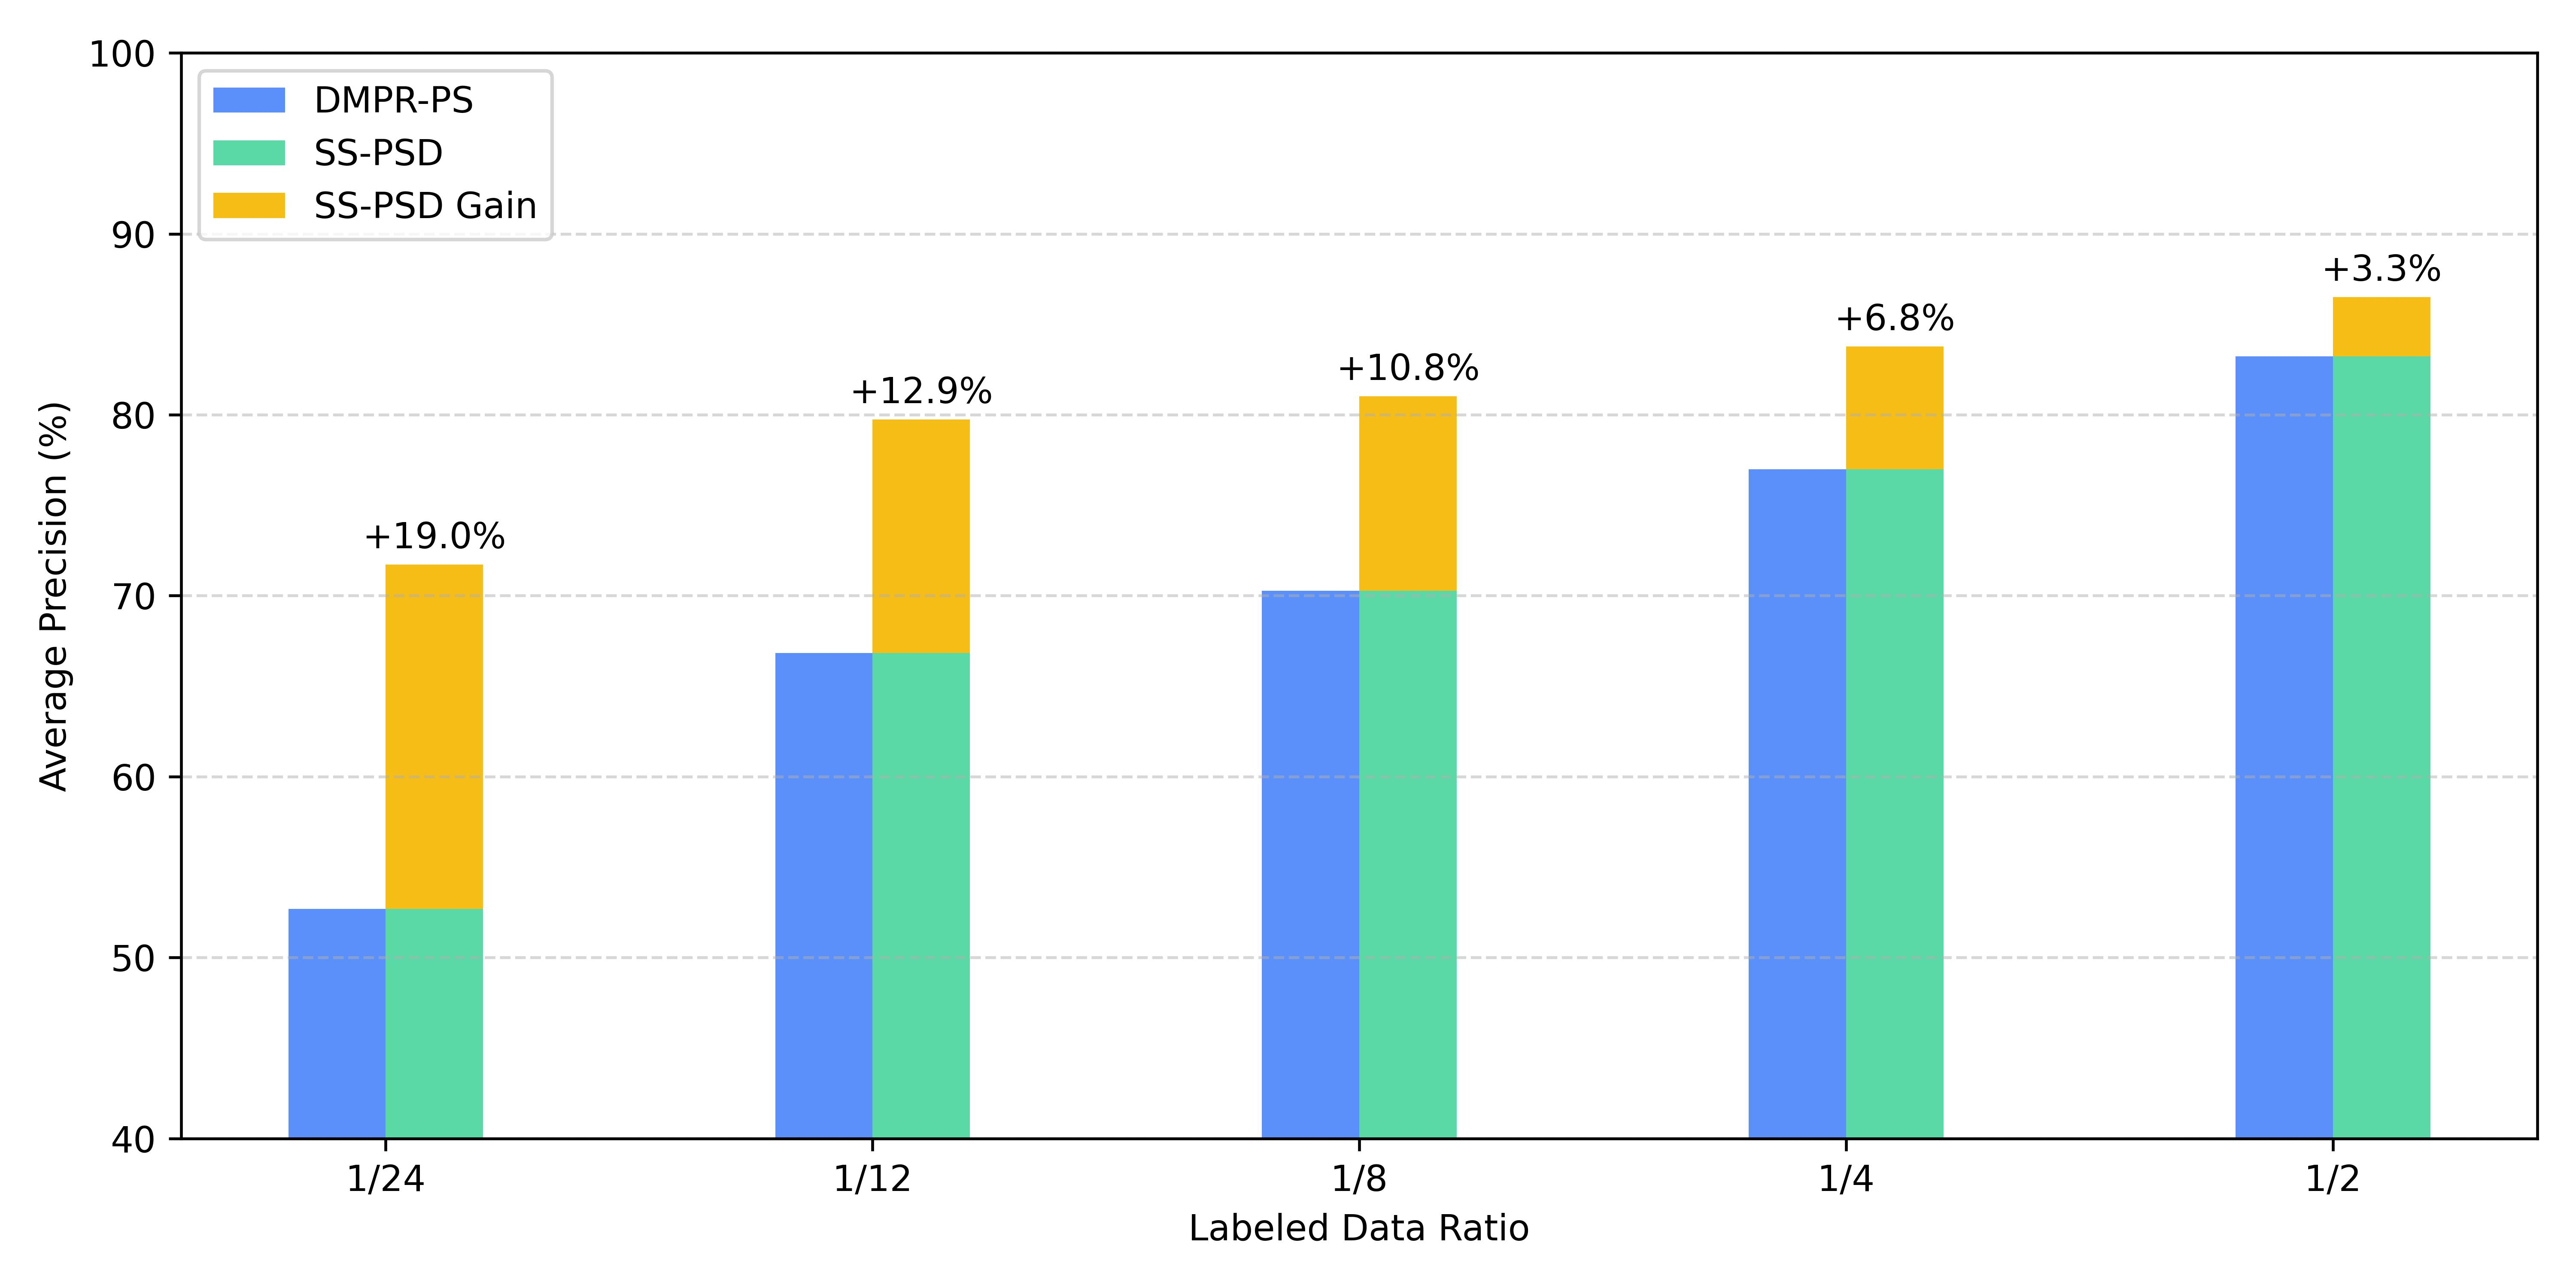
\includegraphics[width=1\linewidth]{figures/chp2/bar/crps.jpg}
    \caption{SS-PSD与DMPR-PS的性能比较（CPRS-D数据集） \\Fig~\ref{fig_crps}~ Performance comparison of SS-PSD and DMPR-PS (CPRS-D dataset)}
    \label{fig_crps}
   \end{figure}

这些结果突出了本文方法在标注数据稀缺场景下的有效性，以及随着监督数据量增加，其可扩展性也得以提升，使其成为标注资源有限的实际应用场景的实用解决方案。 


\subsection{消融实验}
本节探究了置信度引导掩码（CGM）一致性和自适应VAT扰动对所提方法的影响。所有实验均基于CRPS-D数据集展开，标注数据比例设定为1/12。各组成部分的贡献详见表\ref{tab_ab}。本节同时展示了标记点和停车位的检测结果。相较于采用均方误差（MSE）损失的半监督基线MT方法，CGM一致性使停车位检测平均精度（$AP_{parking - slot}$）提升了3.60\%，自适应VAT则可进一步提高0.82\%。

\begin{table}[!h]
\centering
\caption{消融实验结果（1/12标注数据） \\
Table~\ref{tab_ab}~Ablation study using the 1/12 labeled ratio}
\begin{tabular}{cccccc}
\toprule
   有监督基线 & MT & CGM Consistency  & Adaptive-VAT & $AP_{marking-point}$ & $AP_{parking-slot}$ \\
\midrule
    \checkmark  &  &  &  & 72.47\% & 66.84\% \\
     \checkmark & \checkmark &  &  & 78.77\% & 75.33\% \\
     \checkmark & \checkmark & \checkmark &  & 80.86\% & 78.93\% \\
     \checkmark & \checkmark & \checkmark & \checkmark & \textbf{81.59\%} & \textbf{79.75\%} \\
\bottomrule
\end{tabular}
\label{tab_ab}
\end{table}

此外，本节分别针对CGM一致性和Adaptive-VAT进行了消融实验，以进一步验证其有效性。

（1）CGM 一致性

本节深入剖析了各类因素对CGM一致性的影响。首先，去除掩码得到CG一致性，接着去除置信度权重得到C一致性。由表\ref{tab_ablation}可知，对所有单元格施加相同约束以保证一致性，无法取得理想结果（平均精度为55.48\% AP）。然而，借助置信度来指导权重分配，可显著提升结果，而对低置信度区域进行掩码处理，能进一步将结果提升0.71\%。

（2）Adaptive-VAT

若去除Adaptive - VAT的自适应性，其性能会降至 `S-VAT`\cite{tarvainen2017mean}或T-VAT\cite{liu2022perturbed}的水平。
如表\ref{tab_ablation}所示，应用Adaptive-VAT能够获得更优性能，因为它可以在 `S-VAT` 和T-VAT之间自适应地选择更优策略。

\begin{table}[!h]
\centering
\caption{对CGM Consistency和Adaptive-VAT的消融实验 \\
Table~\ref{tab_ablation}~Ablation study of various components on CGM Consistency and Adaptive-VAT}
\setlength{\tabcolsep}{8.0mm}
\begin{tabular}{lcc}
\toprule
  Methods &  $AP_{marking-point}$ & $AP_{parking-slot}$ \\
\midrule
      C consistency &   60.07\% & 54.88\% \\
      CG consistency &   80.75\% & 78.22\% \\
      CGM consistency &  \textbf{81.86\%} & \textbf{78.93\%} \\
\midrule
        S-VAT &   80.97\% & 78.87\% \\
       T-VAT &   81.16\% & 79.53\% \\
        Adaptive-VAT &  \textbf{81.59\%} & \textbf{79.75\%} \\
\bottomrule
\end{tabular}
\label{tab_ablation}
\end{table}

\subsection{超参选择}

本节讨论两个关键超参数的值选择：置信度阈值 ($\tau$) 和干扰强度 ($eps$)。实验均使用 1/12 标注比例在 CRPS-D 数据集上训练。

（1）置信度阈值 ($\tau$)

参考FixMatch\cite{sohn2020fixmatch}的方法（该方法通过选取置信度更高的标签来提升伪标签的准确率），本文设置了较高的阈值（$\tau$ = 0.9）。此外，本文还尝试了将置信度阈值在0到1之间以 0.1 为步长进行变化。如表\ref{tab_confidence}所示，当阈值为0.9时性能最优。 

\begin{table}[!h]
\centering
\caption{不同置信度阈值的实验结果\\
Table~\ref{tab_confidence}~Results of different confidence thresholds.}
    \begin{tabular}{cccc}
    \toprule
    Threshold ($\tau$) & $AP_{marking-point}$ & $AP_{parking-slot}$ & Epochs\\
    \midrule
    0.1 & 81.12\% & 78.81\%	& 36 \\
    0.2	& 81.59\%	& 79.47\%	& 22 \\
    0.3	& 81.28\%	& 79.08\%	& 21 \\
    0.4	& 81.13\%	& 79.34\%	& 23 \\
    0.5	& 81.06\%	& 79.01\%	& 17 \\
    0.6 & 80.75\%	& 79.10\%	& 40 \\
    0.7	& 81.38\%	& 79.50\%	& 23 \\
    0.8	& 80.75\%	& 78.95\%	& 26 \\
    0.9	& \textbf{81.59\%}	& \textbf{79.75\%}	& 22 \\
    \bottomrule
    \end{tabular}
\label{tab_confidence}
\end{table} 

（2）干扰强度 ($eps$)

为证明本文所提Adaptive-VAT算法在各类干扰强度下均能展现优异性能，本文对干扰强度进行了改变，分别采用\(eps\) = 10、1和0.1这几个取值。 

\begin{table}[!h]
\centering
\caption{不同干扰强度的实验结果\\
Table~\ref{tab_eps}~Results of different disturbance intensities}
\begin{tabular}{ccccccc}
\toprule
 & \multicolumn{3}{@{}c@{}}{$AP_{marking-point}$} & \multicolumn{3}{@{}c@{}}{$AP_{parking-slot}$} \\\cmidrule{2-4}\cmidrule{5-7}%
   \multirow{-2}{*}{$eps$}  & S-VAT & T-VAT & Ours & S-VAT & T-VAT & Ours \\
\midrule
    10.0 & 80.89\% & 80.78\% & 81.32\% &79.11\% & 78.89\% & 79.15\%  \\
     1.0 & 80.87\% & 81.04\% & 81.68\% &78.65\% &78.89\% & 79.54\%  \\
     0.1 & 80.97\% & 81.16\% & \textbf{81.59\%} & 78.87\% & 79.53\% & \textbf{79.75\%}  \\
\bottomrule
\end{tabular}
\label{tab_eps}
\end{table}


如表~\ref{tab_eps}所示，与S-VAT和T-VAT相比，本文提出的Adaptive-VAT方法性能更优。基于实验结果，本文最终选择$eps = 0.1$。


\subsection{分场景结果}

表\ref{tab_test}呈现了监督基线方法 (DMPR-PS\cite{huang2019dmpr}) 与本文所提SS-PSD方法在不同场景（对应于CRPS-D数据集的子测试集）下的性能评估情况。该结果基于CRPS-D数据集训练得出，其中标注数据与未标注数据的比例为1/12。无论是在简单场景（如“室内弱光”“室外阴影”），还是复杂场景（如“受损车位”“室外夜晚”），本文模型均展现出更优的性能。停车位检测的可视化结果如图\ref{fig_result}所示。

尤为突出的是，本文的半监督解决方案能够通过有效利用易于获取的未标注数据，显著缓解长尾分布所带来的难题。例如，“室外夜晚”子集的数据规模最小，在监督方案下表现最差，而本文的SS-PSD方法则可大幅提升模型性能。 

\begin{table}[!h]
\centering
\caption{分场景子测试集的实验结果\\
Table~\ref{tab_test}~Evaluation results on the sub-test sets}
\setlength{\tabcolsep}{5.0mm}
\begin{tabular}{lcccc}
\toprule
 \multicolumn{2}{c}{} & \multicolumn{2}{c}{$AP_{parking-slot}\uparrow$} \\ \cmidrule{3-4}%
   \multirow{-2}{*}{场景子集} & \multirow{-2}{*}{图像数} & DMPR-PS$^{*}$ & \textbf{Ours} & \multirow{-2}{*}{提升} \\
\midrule
      室内弱光 & 545  & 74.15\% & 86.68\% & 12.53\%\\
      室内强光 & 786  & 70.00\% & 84.80\% & 14.80\%\\
      阴影 & 1389  & 69.19\% & 81.09\% & 11.90\%\\
      正常日光 & 1703  & 68.06\% & 78.99\% & 10.93\%\\
\midrule
      倾斜车位 & 802  & 61.61\% & 76.79\% & 15.18\%\\
      受损车位 & 302  & 58.90\% & 71.83\% & 12.93\%\\
      雨天 & 323  & 56.07\% & 71.07\% & 15.00\%\\
      夜晚 & 86  & 38.38\% & 63.45\% & \textbf{25.07\%} \\
\bottomrule
\end{tabular}
 \label{tab_test}
\end{table}


\begin{figure}[!h]
\centering
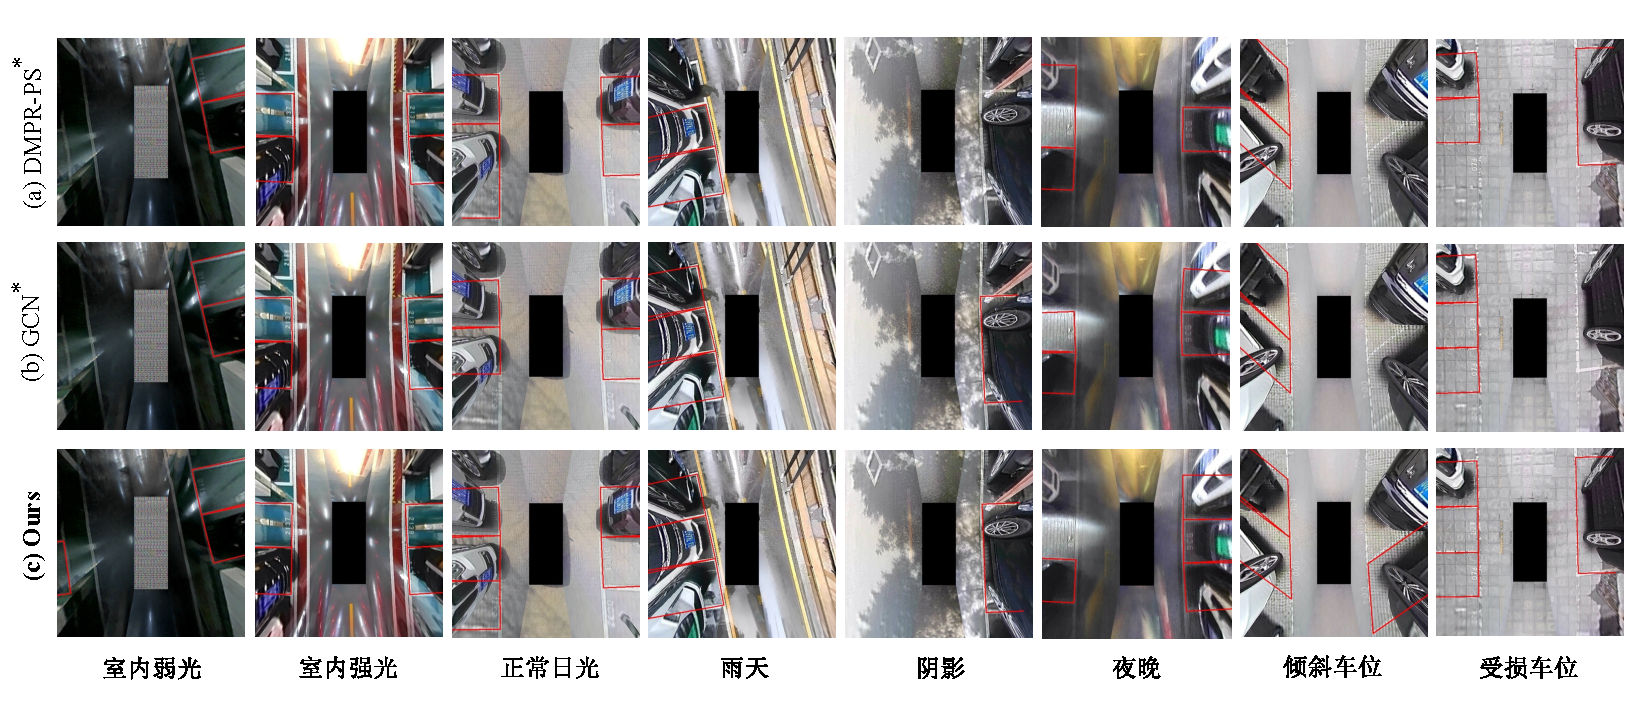
\includegraphics[width=1\textwidth]{figures/chp2/pdf/result.pdf}
\caption{不同场景的可视化结果 \\Fig~\ref{fig_result}~Visualized results of different scenes}
\label{fig_result}
\end{figure}



\section{本章小结}

本章聚焦于复杂真实场景中停车位检测任务面临的数据规模受限以及标注成本高昂问题，构建了一个大规模停车位数据集。该数据集覆盖多光照、多视角以及多停车形式，为后续方法研究搭建了统一的数据基础。此数据集包含在各类天气条件下拍摄的鸟瞰图像，涵盖多种场景。相较于以往数据集，它更具挑战性，不仅规模更大、场景更多样，倾斜停车位比例更高，还包含更多标线损坏的复杂实例。此外，本章提出一种面向停车位检测任务的半监督检测框架，借助教师-学生学习范式，有效运用未标注数据，提升模型的泛化能力与鲁棒性。

本章工作从数据与学习范式两个层面，缓解了停车位检测在复杂场景下的训练瓶颈，为后续基于单帧与多帧建模的检测方法，奠定了坚实的数据与训练基础。 


 								%第二章
	%  \setlength{\baselineskip}{20pt}
\chapter{单帧结构感知的端到端停车位检测方法}
\label{cha:chap3}

\section{研究动机}
随着智能驾驶技术的快速发展，自动泊车系统已成为提升驾驶便利性与安全性的关键模块，而停车位检测作为自动泊车感知系统的基础，其准确性直接决定了泊车路径规划与运动控制的可靠性。

在前一章成功构建大规模停车位数据集 CRPS-D 并提出半监督训练框架 SS-PSD 的基础上，如何进一步提升停车位检测在单帧条件下的结构表达能力成为新的关键挑战。停车位本质上由多个关键点及其几何关系共同定义，具有显著的结构属性，但部分现有方法仍将停车位检测视为局部特征预测问题，依赖启发式规则对检测结果进行后处理组合，导致结构一致性难以保证，在停车位密集或局部遮挡场景下容易出现匹配错误。

从建模角度深入分析，停车位检测的核心难点不在于单个关键点的定位精度，而在于关键点之间结构关系的合理建模与约束。若结构信息未能在训练阶段得到充分利用，即便单点检测精度较高，也难以保证最终检测结果的整体结构一致性与稳定性。因此，有必要从建模范式上重新审视停车位检测问题，将结构约束显式引入模型优化过程。

当前端到端检测框架普遍面临三个主要问题：一是关键点之间的结构关系建模不充分，导致复杂拓扑下车位边界易重构错误；二是环境变化带来的样本异质性显著，如低光照、遮挡或背景干扰等情况会影响模型对局部关键点特征的准确感知；三是现有训练策略与损失函数多关注点位回归准确性，忽视点间拓扑一致性约束，无法有效引导模型学习更具结构感知能力的表示。

针对上述问题，本章提出单帧结构感知的端到端停车位检测方法，该方法以关键点表示为核心，通过在端到端训练过程中引入停车位内部结构关系约束，实现关键点定位与结构匹配的联合优化，避免对启发式后处理规则的依赖，为复杂场景下的停车位检测提供更加稳定一致的单帧建模方案。

具体而言，在检测框架设计中引入结构建模增强机制以提升车位重构稳定性，同时从损失函数与数据增强角度出发，设计结构感知的训练优化策略，以更好适应实际场景中结构不完整、样本稀疏与干扰显著的问题。综合实验验证表明，该方法在多种典型复杂环境下均具备良好的检测精度与稳定性，展现出较强的实际应用潜力。


\section{方法介绍}

本节详细介绍单帧结构感知的端到端停车位检测方法，该方法旨在解决复杂环境下停车位的稀疏关键点检测与结构匹配问题，通过引入结构感知的数据增强策略、特征插值机制与稀配聚焦损失函数，有效提升模型在低标注密度下的鲁棒性与泛化能力。

\subsection{模型框架}


\begin{figure}[!h]
\centering
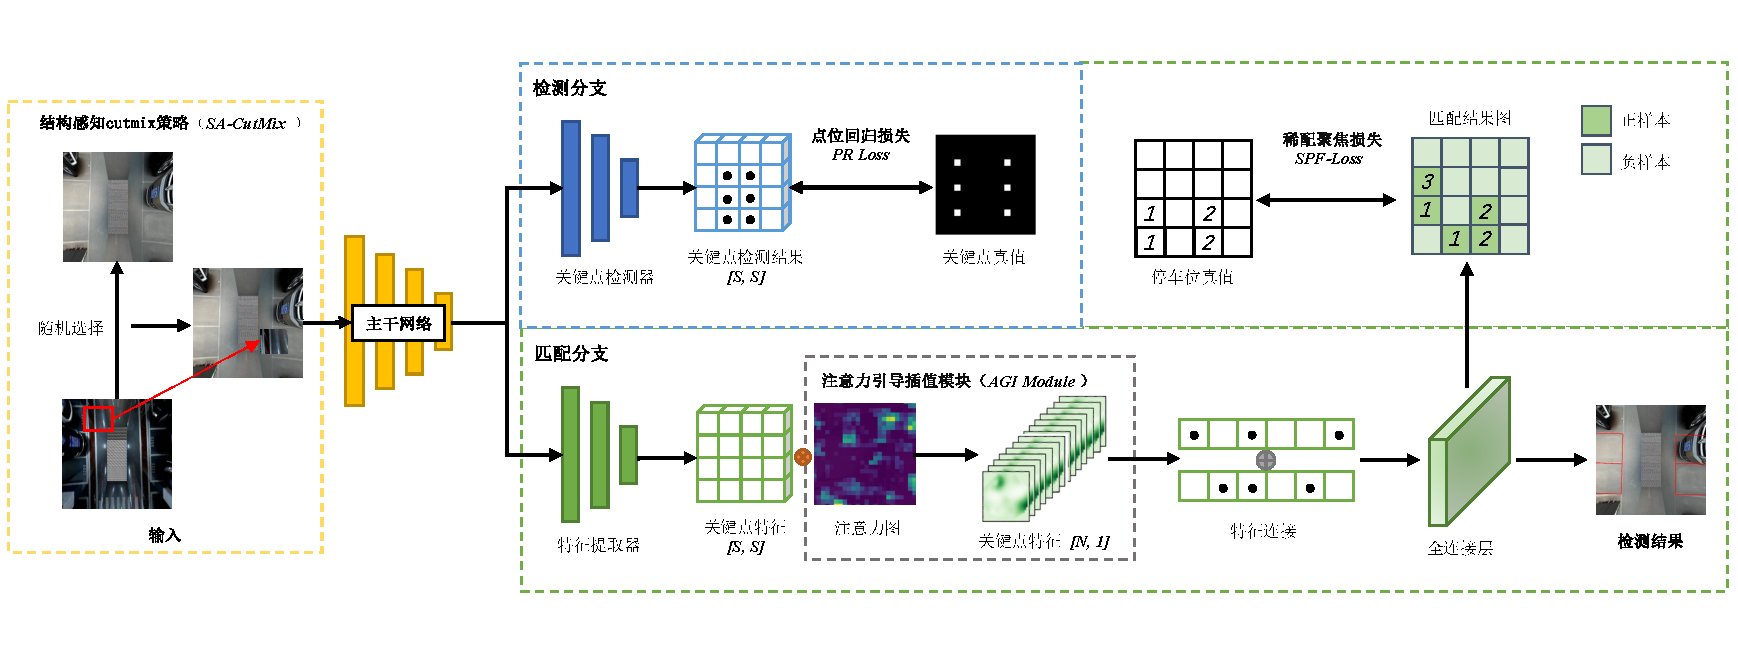
\includegraphics[width=1\textwidth]{figures/chp3/pipline_2.pdf}
\caption{单帧结构感知的端到端停车位检测框架示意图 \\Fig~\ref{fig_pip2}~Overview of the single-frame structure-aware end-to-end parking slot detection framework}
\label{fig_pip2}
\end{figure}

如图 \ref{fig_pip2} 所示，所提出的方法采用双分支架构，包含关键点检测分支与匹配分支。关键点检测分支负责提取图像中的停车位关键点位置，匹配分支则基于检测结果构建候选点对，进行结构匹配判断并生成最终停车位位置。输入图像首先经过主干特征提取网络处理，随后分流至两个分支执行各自任务。

为提升模型的结构感知能力与鲁棒性，该框架引入三项核心设计：

\textbf{结构感知 CutMix 策略（Structure-Aware CutMix，SA-CutMix）}：通过在背景区域进行智能裁剪替换，增强背景多样性的同时保持关键点结构完整性，提高模型对非结构区域的鲁棒性。

\textbf{注意力引导插值模块（Attention-Guided Interpolation，AGI Module）}：利用注意力机制引导特征插值，提升特征对关键结构位置的敏感性与表示能力。

\textbf{稀配聚焦损失（Sparse Pairwise Focal Loss，SPF-Loss）}：针对停车位关键点稀疏分布的特点，设计聚焦损失函数，缓解样本稀疏带来的训练不稳定问题。

下面将依次对这三个关键组件进行详细阐述。

\subsection{结构感知CutMix策略}
在关键点检测任务中，数据分布不均衡与场景复杂性会对模型泛化能力造成挑战，数据增强策略因此成为训练过程的关键组成部分。CutMix\cite{yun2019cutmix} 是一种经典的增强方法，通过在不同图像间随机裁剪并粘贴区域，线性混合标签信息，显著提升模型鲁棒性与抗过拟合能力。然而，原始 CutMix 未考虑空间结构语义，直接随机裁剪替换区域，在结构化感知任务中可能引发严重问题。

\begin{figure}[!h]
\centering
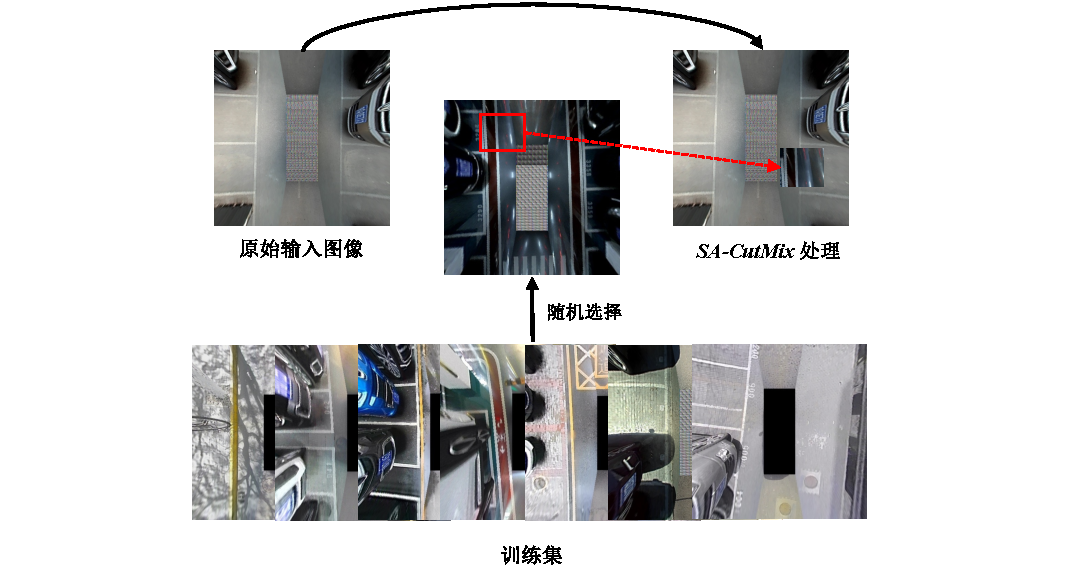
\includegraphics[width=1\textwidth]{figures/chp3/sa.pdf}
\caption{结构感知 CutMix 策略示意图 \\Fig~\ref{fig_cutmix}~Illustration of the Structure-Aware CutMix strategy}
\label{fig_cutmix}
\end{figure}

以停车位关键点检测为例，关键点稀疏且结构性强，具有明确的几何构型与位置分布规律。原始 CutMix 可能无意中裁剪关键点所在区域，打断空间几何关系，使模型难以学习结构先验，影响定位精度与稳定性。
为克服上述局限，本文提出结构感知 CutMix 策略（SA-CutMix），旨在保留结构语义信息的同时引入多样化背景扰动，兼顾数据多样性与几何结构稳定性。SA-CutMix 的核心理念是仅在背景区域进行替换操作，避免破坏关键点区域的空间结构特征。图\ref{fig_cutmix}展示了 SA-CutMix 的整体流程。

具体而言，对于每张训练图像，SA-CutMix 首先提取所有标注关键点的坐标信息，然后随机采样矩形裁剪区域作为候选替换区域。对每个候选区域，检查是否与关键点区域重叠，若有交集则视为包含结构语义信息，直接舍弃。仅当候选区域完全处于背景区域（不包含任何关键点）时，才从另一张随机选取的图像中提取相同大小的图像块进行粘贴替换。为确保算法效率，设置最大尝试次数，若未能采样到合法区域则跳过本轮增强。

该策略可概括为如下伪代码流程：

\begin{algorithm}[htbp]
\caption{结构感知 CutMix 数据增强（SA-CutMix）}
\label{alg:sacutmix}
\begin{algorithmic}[1]
\Require 当前样本图像 $I_1$，关键点坐标 $M_1$，数据集 $\mathcal{D}$
\Ensure 增强后的图像 $I_{\text{mix}}$
\If{$|\mathcal{D}| < 2$}
    \State \Return $(I_1, M_1)$ \Comment{样本不足，跳过 CutMix}
\EndIf
\Repeat
    \State 从 $\mathcal{D}$ 中随机选择 $(I_2, M_2)$，且 $I_2 \neq I_1$
    \State 在图像中随机生成矩形区域 $(x, y, w, h)$
\Until{该区域不包含 $M_1$ 中的关键点}
\State 用 $I_2$ 中对应区域替换 $I_1$ 中 $(x:x+w, y:y+h)$ 区域
\State 得到增强图像 $I_{\text{mix}}$
\State \Return $(I_{\text{mix}}, M_1)$
\end{algorithmic}
\end{algorithm}
 
SA-CutMix 从结构保持与信息干扰两个角度出发：一方面保留关键点对应的几何结构区域，使模型持续学习结构先验；另一方面引入其他图像的背景扰动，如不同地面材质、纹理变化、光照条件或遮挡物体，有效扩展模型对环境变化的感知能力。
与原始 CutMix 相比，SA-CutMix 更适用于关键点稀疏、结构约束强的任务场景。在停车位检测中，关键点数量有限且排列规律显著，任何对结构区域的破坏都可能导致空间推理能力下降。SA-CutMix 避免了这种破坏，在结构稳定的前提下引入背景扰动，增强模型对边缘遮挡、复杂纹理与极端光照等复杂场景的适应能力。

实验评估表明，SA-CutMix 的引入对模型性能具有显著提升作用。在多个遮挡与干扰条件下，模型的定位准确性与边界鲁棒性均有提升，验证了该策略在结构感知数据增强中的有效性与普适性。

\subsection{注意力引导插值模块}
在停车位关键点检测与匹配任务中，特征的精细建模对于稀疏关键点的准确定位与结构关系的稳定建模至关重要。传统描述符提取方法多采用直接在特征图上进行双线性插值采样的方式，尽管具备一定的连续性和可微性，但对所有空间位置一视同仁，未能显式区分结构区域与背景区域的重要性差异。在复杂场景中，如存在遮挡、强光、阴影或纹理混杂等干扰时，这种等权采样机制往往会削弱关键结构区域的表达能力，导致描述符判别性不足，影响后续的匹配与回归性能。

为此，本文提出注意力引导的特征插值模块（AGI Module），通过引入轻量注意力机制提升特征在结构区域的表达能力，增强描述符对结构关系的建模效果。具体地，设输入特征图为 $F\in R^{B\times C\times H\times W}$，其中 $B$ 为 batch 大小，$C$ 为通道数，$H,W$ 为特征图尺寸。首先通过 $1\times1$ 卷积操作提取通道注意力响应，生成单通道注意力图 $A\in R^{B\times1\times H\times W}$，并使用 Sigmoid 激活函数将其归一化至区间 $\left[0,1\right]$，以获得每个空间位置的显著性估计：
\begin{equation}
    A=\sigma\left({\mathrm{Conv}}_{1\times1}\left(F\right)\right)
\end{equation}

该注意力图反映当前图像中结构区域的重要性分布，可用于强调具有结构语义的显著区域并抑制冗余或噪声背景。随后，原始特征图与注意力图逐元素相乘，得到加权特征图 $F\prime=F\odot A$，该操作在保留空间连续性的同时增强了结构敏感区域的响应，有助于提升后续插值描述符的判别性。

在加权特征图 $F\prime$ 上，继续采用双线性插值对关键点位置进行特征采样。考虑到关键点位置以归一化坐标 $\left[-1,1\right]$ 表示，具体采样过程通过 PyTorch 的 $F.grid\_sample$ 函数实现，并将结果沿空间维度展平，得到结构感知描述符 $D\in R^{B\times C\times N}$，其中 N 表示每张图像中的关键点数量。由于注意力机制已对特征图进行重加权，该描述符在稀疏标注条件下表现出更强的稳定性与区分能力。整个过程如图\ref{fig_agi}所示：

\begin{figure}[!h]
\centering
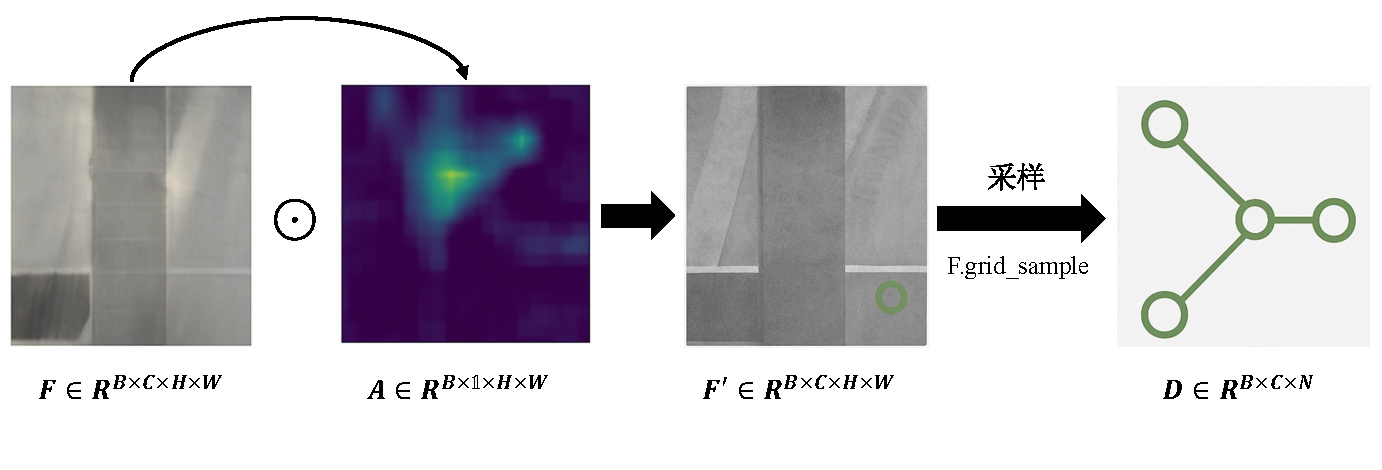
\includegraphics[width=1\textwidth]{figures/chp3/agi.pdf}
\caption{注意力引导插值模块示意图 \\Fig~\ref{fig_agi}~Illustration of the Attention-Guided Interpolation Module}
\label{fig_agi}
\end{figure}

与传统直接插值方法相比，AGI 模块通过显式建模区域重要性信息，引导描述符采样过程更加聚焦于结构显著区域，避免了背景干扰对特征表达的稀释效应。同时，AGI 模块设计简单、计算开销极小，易于集成到现有网络结构中并保持端到端训练流程。在实际停车位检测任务中，该模块在多个复杂环境下均展现出良好的泛化能力和鲁棒性，实验结果表明其对关键点检测精度和匹配稳定性均具有显著提升，进一步验证了结构引导特征建模在场景感知任务中的重要性与有效性。

\subsection{损失函数设计}
在端到端的停车位检测任务中，模型需要同时具备两项核心能力：一是精确预测图像中的停车位关键点位置，二是正确判断关键点之间是否属于同一停车位的结构关系。这两个子任务分别对应空间定位与结构理解两个方向，是最终构建完整停车位边界的必要前提。

为此，本文设计了专门的监督机制：点位回归损失（Point Regression Loss, PR-Loss）和稀配聚焦损失（Structure-aware Pairwise Focal Loss, SPF-Loss）。通过联合优化这两个损失项，模型能够在空间定位和结构关系建模两个层面上同步学习，获得更加完整和鲁棒的停车位检测能力。

（1）点位回归损失（PR-Loss）

为实现像素级的关键点定位精度，本文引入点位回归损失，用于监督模型精确预测关键点在特征图中的空间分布。该损失直接作用于从注意力增强后的特征图中回归出的置信度图及偏移信息。

本文将关键点表示为三通道张量：第一通道为关键点存在的置信度，后两通道为相对偏移 x,y。标签张量与 mask 通过以下策略构建：

a.置信度通道中，仅在真实标记点位置处置为 1；

b.偏移通道中记录该点在网格内的相对偏移；

c.mask 中标记出参与训练的位置，用于规避空区域的梯度干扰。


模型输出的点位预测结果与标签进行逐点比较，计算方式如下：
\begin{equation}
    \mathcal{L}_\mathrm{\mathrm{PR}}=\frac{1}{N_{\mathrm{mask}}}\left.\ |\left(\hat{T}-T\right)\odot M\right.|_2
\end{equation}

其中，$\hat{T}, T\in R^{B\times3\times H\times W}$ 分别表示预测与标签张量，$M$ 为 mask，$\odot$ 表示逐元素乘法，$N_{\mathrm{mask}}$ 为 mask 中非零位置的数量。损失计算时分别对置信度与偏移误差加权平均。该设计不仅提升了关键点位置的回归精度，同时使模型在关注结构区域时具备更强的几何稳定性，进一步增强了特征匹配的定位一致性。

（2）稀配聚焦损失（Structure-aware Pairwise Focal Loss, SPF-Loss）

关键点匹配任务本质上可视为一个二分类问题，即判断任意两个候选关键点是否构成真实匹配对。传统方法常采用 Binary Cross Entropy（BCE）损失，但在“结构模糊区域”中，例如存在遮挡、模糊或车位密集的情况下，模型往往难以聚焦于困难样本，容易出现误匹配。为此，本文提出稀配聚焦损失（SPF-Loss），引入焦点机制增强对难匹配样本的关注，同时结合结构约束以提升对稀疏边对的判别能力，从而提高整体匹配精度与鲁棒性。

具体而言，首先构建大小为 $N \times N$ 的匹配预测矩阵 $P=\{p_{ij}\}$，其中每个元素表示图像对中第 i 个关键点与第 j 个关键点的匹配置信度。同时构建标签矩阵 $Y=\{y_{ij}\}$，其中 $y_{ij}=1$ 表示正匹配对，$y_{ij}=2$ 表示负匹配对，$y_{ij}=0$ 表示无效对。此外，定义有效掩码 $M_{ij}=\mathbb{1}\left(y_{ij}>0\right)$，仅对有效匹配对（正负样本）计算损失，以排除对模型无意义的区域干扰。

本文采用 Focal Loss\cite{lin2017focal} 的形式，将传统 BCE 扩展为：
\begin{equation}
    \mathcal{L}_\mathrm{SPF}=-\frac{1}{N_{\mathrm{valid}}}\sum_{i,j} M_{ij}\cdot\left[\alpha\left(1-p_{ij}\right)^\gamma y_{ij}^\prime\log{\left(p_{ij}+\varepsilon\right)}+\alpha p_{ij}^\gamma\left(1-y_{ij}^\prime\right)\log{\left(1-p_{ij}+\varepsilon\right)}\right]
\end{equation}

其中，$p_{ij}$ 表示模型预测的匹配概率，$\alpha$ 为类别权重调节因子，$\gamma$ 控制聚焦程度，$\varepsilon$ 是为防止数值不稳定引入的微小常数，$N_{\mathrm{valid}}$ 为所有有效点对数量。由于 Focal Loss 是专为二分类任务设计的，其要求标签为二值形式（正样本为 1，负样本为 0），因此构造二值化目标标签：
\begin{equation}
    y_{ij}\prime=\mathbb{1}\left(y_{ij}=1\right)
\end{equation}

即当 $y_{ij}=1$ 时，$y_{ij}\prime = 1$；否则为 0。该设计不仅解决了原始多标签匹配信息与 Focal Loss 结构不兼容的问题，同时避免了无效区域带来的梯度干扰，使得模型能更加关注边界模糊、结构遮挡、复杂形状干扰等困难匹配场景，训练过程中自动对高难度匹配对赋予更大梯度，从而显著提升结构推理能力。

（3）总损失函数

上述两种损失在训练过程中被共同优化，整体损失函数形式为：
\begin{equation}
    \mathcal{L}_\mathrm{total}=\lambda_1\cdot\mathcal{L}_\mathrm{PR}+\lambda_2\cdot\mathcal{L}_\mathrm{SPF}
\end{equation}

其中，$\lambda_1、\lambda_2$为损失项的加权系数，用于平衡结构判别与点位回归的相对重要性。实验表明，该损失设计能够有效提升模型在复杂环境下的匹配鲁棒性与几何一致性，尤其在面对结构遮挡、视角变化或多目标干扰等挑战性场景时，性能提升显著。本文选取在验证集上综合性能最优的一组权重参数，并在所有实验中保持一致。最终，点位回归损失与结构感知匹配损失的权重分别设置为 $\lambda_1 = 10，\lambda_2 = 1$。

\section{实验结果及分析}
本章所有实验均在同一硬件平台上进行，具体包括一块Nvidia 2080Ti GPU（12GB显存）和一台配备Intel(R) Xeon(R) E5-2680 v4 @ 2.40GHz CPU的服务器环境。模型训练使用PyTorch框架实现。

\subsection{对比实验}
（1）公开数据集 ps2.0

为验证所提方法的有效性，本文首先在公开数据集 ps2.0 上进行了充分的对比实验。ps2.0 数据集作为当前视角停车位检测任务中最具代表性和广泛使用的基准数据集之一，涵盖了多种典型的室内外停车场景，被众多主流方法用于性能评估。该数据集中，已有方法的检测精度普遍较高，查准率（Precision）和查全率（Recall）均达到 99\%左右，整体性能趋于饱和。

\begin{table}[!ht]
\centering
\setlength{\tabcolsep}{5mm}
\caption{不同方法在 ps2.0 数据集上的检测性能对比 \\
Table~\ref{tab_2ps2}~Comparison of detection performance of different methods on ps2.0 dataset}
\begin{tabular}{lccccc}
\toprule
    方法 &  Precision & Recall &  AP\\
\midrule
       DeepPS\cite{zhang2018vision}  &  98.99\% & 99.13\% & / \\
       DMPR-PS\cite{huang2019dmpr} &  99.42\% & 99.37\% & / \\
       VPS\cite{li2020vacant}  &  99.63\% & 99.10\% & / \\
       GCN\cite{min2021attentional}  &  99.56\% & 99.42\% & /\\
       SCCN \cite{zheng2022center}  &  99.35\% & 99.17\% & / \\
       Bui et al.\cite{bui2023one} &   99.63\% & 99.63\% & / \\
       SAM-PS\cite{zhai2024sam} &  94.29\% & 81.35\% & / \\
       BEV-PolyNet\cite{duan2025bev}  &  99.82\% & 99.65\% & / \\
       \textbf{Ours} &   \textbf{99.37\%} & \textbf{99.47\%} & \textbf{99.47\%}\\
\bottomrule
\end{tabular}
\label{tab_2ps2}
\end{table}

如表\ref{tab_2ps2}所示，本文方法在 ps2.0 数据集上的查准率为 99.37\%，查全率为 99.47\%，与现有先进方法保持在同一水平，充分验证了所提出方法在标准场景下的适应性和准确性。值得注意的是，本文方法是唯一在该数据集上提供平均精度（AP）指标的方法，达到了 99.47\%，进一步印证了模型在检测精度与鲁棒性方面的兼顾能力。

然而，ps2.0 数据集中场景较为规整，泊车线条清晰、遮挡情况较少，难以覆盖真实自动泊车场景中可能遇到的复杂情况，如遮挡严重、停车位密集、斜向车位增多等。因此，仅在该数据集上取得良好性能并不足以全面评估模型在真实环境中的实际应用潜力。为此，本文进一步引入具有更高挑战性和复杂度的私有数据集 CRPS-D，并在该数据集上进行了更具代表性的对比实验，以验证所提方法在复杂场景下的泛化能力与鲁棒性。

（2）新数据集CRPS-D

在进一步的实验中，本文在上一章构建的CRPS-D数据集上对所提方法进行了深入评估。鉴于目前大多数端到端停车位检测方法尚未公开训练代码或预训练模型，难以在统一平台和设置下在CRPS-D上实现全面复现与公平对比。在已公开的方法中，仅有GCN\cite{min2021attentional}提供了完整的训练框架，并支持多种主干网络（ResNet18、ResNet50、Darknet、VGG16），具备良好的可复现性与扩展性。因此，本文选取GCN作为对比基线，在保持数据集、损失函数、训练策略和超参数一致的前提下，基于相同的四种主干网络在CRPS-D数据集上进行了复现训练，并与本文方法进行了系统的对比实验。

\begin{table}[!h]
\centering
\setlength{\tabcolsep}{4mm}
\caption{本文方法与 GCN\cite{min2021attentional} 在 CRPS-D 数据集上的检测性能对比 \\
Table~\ref{tab_2crps}~Comparison between the proposed method and GCN\cite{min2021attentional} on CRPS-D dataset}
    \begin{tabular}{lccccc}
        \toprule
         方法 & 主干网络 & Precision & Recall & AP & AP提升 \\
        \midrule
            GCN$^{*}$  & \multirow{2}{*}{Resnet18} & 91.38\% & 82.04\% & 78.01\%  & \multirow{2}{*}{4.37\%}\\
             本文方法  &  & 91.56\%	& 84.54\%	& 82.38\%  & \\

        \midrule
             GCN$^{*}$  & \multirow{2}{*}{Resnet50} & 90.91\%	& 83.22\%	& 78.63\%  & \multirow{2}{*}{3.47\%}\\
             本文方法  &  & 91.11\% &	84.89\%	& 82.10\%	  & \\
        \midrule
              GCN$^{*}$  & \multirow{2}{*}{Darknet} & 91.38\%	& 83.27\%	& 79.01\%  & \multirow{2}{*}{3.92\%}\\
             本文方法  &  & 91.39\% &	85.00\%	& 82.93\%	  & \\
        \midrule
              GCN$^{*}$  & \multirow{2}{*}{Vgg16} & 92.43\%	& 82.75\%	& 79.02\%  & \multirow{2}{*}{4.56\%}\\
             本文方法  &  & 92.21\%	& 85.54\%	& 83.58\%  & \\
        \bottomrule
    \end{tabular}
    \label{tab_2crps}
\end{table}

实验结果如表\ref{tab_2crps}所示，本文方法在四种主干网络下均实现了对 GCN 方法的全面超越，特别是在关键指标 AP 上取得了显著提升。其中，基于 VGG16 的配置下，本文方法的 AP 达到 83.58\%，相较 GCN 的 79.02\%，提升了 4.56 个百分点，体现出在较深网络结构下的更强表达能力。在 ResNet18、ResNet50 和 Darknet 主干下，AP 也分别提升了 4.37\%、3.47\% 和 3.92\%，平均提升约 4.08\%。该结果表明，本文方法在不同主干结构下均具备良好的兼容性和稳定性，能够有效挖掘停车位的结构信息，提升检测性能。

此外，从表格数据可以看出，在查准率保持相对稳定的同时，本文方法在查全率方面有明显增长。例如，在 VGG16 主干下，查全率从 82.75\% 提升至 85.54\%，增长了 2.79 个百分点；在 ResNet18 主干下，查全率从 82.04\% 提升至 84.54\%，增长了 2.50 个百分点。这表明本文方法在面对复杂、密集、非规则停车位分布场景时，具备更强的目标捕获能力，同时保持了较高的检测精度。这种能力的提升对于实际自动泊车系统中的可靠检测至关重要，特别是在遮挡、光照变化、车位倾斜和空间紧凑等真实条件下。

\subsection{消融实验}

为进一步验证本文所提出各模块与设计的有效性，本文在 CRPS-D 数据集上进行了消融实验。实验采用ResNet18作为主干网络，依次引入关键设计组件，包括 AGI模块、 SPF-loss 以及 SA-CutMix 数据增强策略，并在保持其他设置不变的前提下，观察各组件对模型性能的影响。实验结果如表 \ref{tab_2ab} 所示。

\begin{table*}[!h]
\centering
\setlength{\tabcolsep}{4mm}
\caption{模块逐步引入对模型性能的影响 \\
Table~\ref{tab_2ab}~Impact of incremental module integration on detection performance}
\small
\begin{tabular}{ccccc}
\toprule
    Baseline(仅主干网络) & AGI Module & SPF-Loss  & SA-CutMix &  $AP_{parking-slot}$ \\
\midrule
    \checkmark  &  &  &  &  77.76\% \\
     \checkmark & \checkmark &  &  &  78.94\% \\
     \checkmark & \checkmark & \checkmark &  &  79.45\% \\
     \checkmark & \checkmark & \checkmark & \checkmark  & \textbf{82.38\%} \\
\bottomrule
\end{tabular}
\label{tab_2ab}
\end{table*}

从实验结果可以看出，所提出的每个模块均对最终性能有积极贡献，且呈现出累加效应。首先，在基准模型中引入AGI模块后，AP从 77.76\%提升至 78.94\%，提升了 1.18 个百分点，表明该模块在捕捉车位关键点间的几何关系方面具备良好的建模能力。进一步加入 SPF-Loss 后，AP 提升至 79.45\%，显示结构感知损失函数能有效增强模型对关键点间结构匹配的关注，从而提高整体检测精度。最后，结合 SA-CutMix 数据增强策略后，AP 显著提升至 82.38\%，进一步提升了模型的泛化能力和鲁棒性。

综上所述，本文各关键设计均能在不同程度上提升模型性能，且组合使用时效果最优，验证了本文提出方法在结构建模、损失设计和数据增强等方面的有效性和互补性。各模块协同工作，共同提升了模型在复杂场景下的检测性能。

\subsection{可视化结果}
为进一步验证本文方法在实际应用中的泛化能力与鲁棒性，本文从 CRPS-D 数据集中选取了十种具有代表性的复杂场景进行可视化展示，如图 \ref{fig_res2} 所示。所选场景涵盖了多种真实环境下的典型干扰因素，包括光照条件多变（如室内弱光、强光、夜间和强阴影）、恶劣天气（如雨天）、结构复杂性（如斜置车位和受损车位），以及车位分布密集或地面存在反光等情形。这些场景充分模拟了实际停车环境中常见的挑战因素，对模型的感知能力和鲁棒性提出了更高要求。

\begin{figure}[!h]
\centering
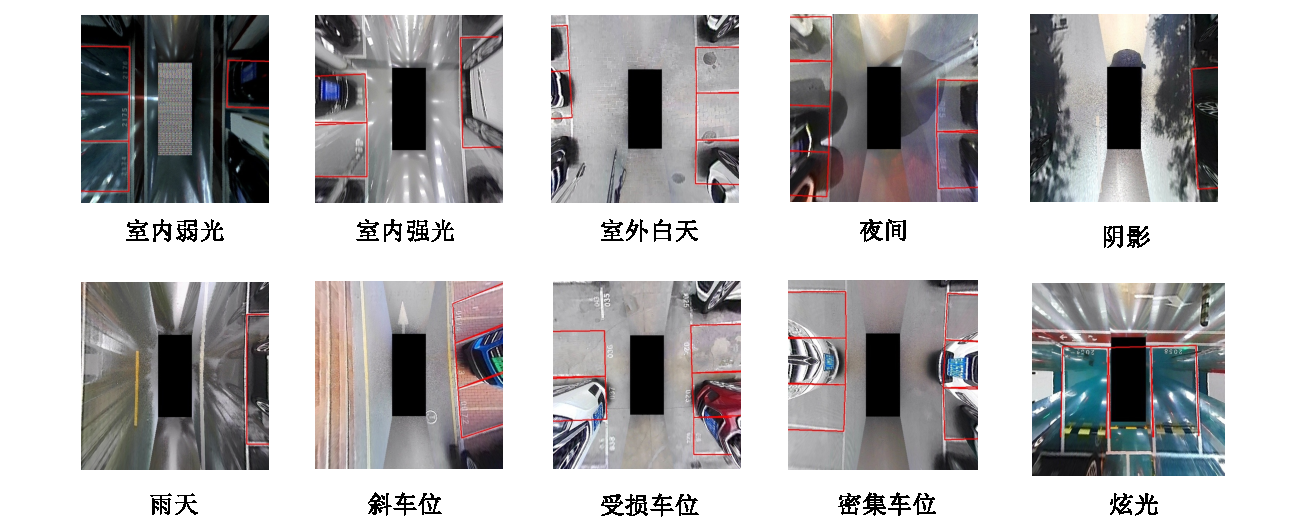
\includegraphics[width=1\textwidth]{figures/chp3/result_2.pdf}
\caption{不同场景下的可视化停车位检测结果 \\Fig~\ref{fig_res2}~Visualization results of parking slot detection under diverse scenarios}
\label{fig_res2}
\end{figure}

从图 \ref{fig_res2} 结果可以看出，本文方法在各类复杂条件下均能准确检测车位关键点，并有效构建出完整的车位结构。即使在光照不足、强反光或雨天等视觉干扰较强的场景中，检测结果仍然清晰、边界准确，未出现明显误检或漏检，展示了良好的环境适应性和稳定性。同时，在车位密集和斜置等边界难以区分的复杂场景中，方法仍表现出较高的判别能力，进一步验证了其在多样化泊车环境下的应用潜力。这些可视化结果与定量实验数据相互印证，充分展示了本文方法的有效性和鲁棒性。

\section{本章小结}

本章针对单帧条件下停车位检测中结构表达能力不足的问题，提出了一种单帧结构感知的端到端停车位检测方法，实现了关键点定位与结构匹配的联合优化。

该方法设计了双分支检测框架，通过关键点检测分支与匹配分支的协同工作，在无需额外后处理的情况下自动构建车位结构，有效融合了车位拓扑先验信息。同时，提出了三项核心技术：结构感知CutMix策略（SA-CutMix）在保持结构完整性的同时增强模型泛化能力；注意力引导插值模块（AGI Module）提升特征对结构区域的敏感性；稀配聚焦损失（SPF-Loss）增强模型对困难样本的判别能力。

实验验证表明，该方法在ps2.0和CRPS-D数据集上均取得了优异性能，在 CRPS-D 数据集上相比基线方法平均提升 AP 约 4.08\%，尤其在复杂场景下表现出更强的鲁棒性。消融实验进一步验证了各模块的有效性，其中 SA-CutMix 带来约 2.93\% 的 AP 提升，AGI模块带来约 1.18\% 的AP提升，SPF-Loss 带来约 0.51\% 的 AP 提升。

本章方法通过显式引入结构约束，有效提升了停车位检测在遮挡、密集与非标准停车形式下的稳定性与一致性，为后续引入时序信息提供了可靠的单帧结构基础。 								%第三章
	%  \setlength{\baselineskip}{20pt}
\chapter{多帧时序特征融合的停车位检测方法}
\label{cha:chap4}



\section{研究动机}
在真实停车场景中，环视相机采集的连续帧图像存在明显的时序相关性。尽管单帧结构感知检测方法能够在静态图像条件下有效提升停车位检测的结构一致性，但在真实驾驶与泊车过程中，车辆获取的是连续帧视觉信息。受视角变化、动态遮挡以及环境噪声等因素影响（停车位位置在相邻帧中基本稳定，仅光照、阴影、遮挡略有变化，而噪声、反射或标线模糊在单帧中可能导致检测不稳定），现有方法仅基于单帧特征进行检测，忽略了时序上下文信息，导致在动态场景（光照闪烁、行人经过等）下精度波动。

从任务本质上看，停车位检测并非完全静态的问题，而是具有明显的时序属性。相邻帧之间在空间结构和语义信息上具有高度相关性，合理利用时序信息有助于弥补单帧检测在复杂场景中的不确定性。然而，现有研究中对停车位检测时序建模的关注仍相对有限，如何在保持端到端检测流程的同时，引入有效的时序特征融合机制，仍有待进一步探索。

本章在单帧结构感知检测方法的基础上，进一步将停车位检测问题从静态图像建模扩展至多帧时序建模。通过对连续帧中结构感知表示进行时序特征融合，显式建模停车位在时间维度上的一致性，有效缓解了单帧检测中由遮挡与视角变化引起的不稳定问题。该方法从建模维度上实现了由空间结构感知向时空联合感知的扩展，使停车位检测更加贴近真实驾驶场景。




\section{方法介绍}
如图\ref{fig_pip3}所示，多帧时序特征融合的停车位检测方法在单帧结构感知检测框架的基础上，引入了跨时帧自注意力机制和时序一致性约束，实现了时空联合感知的停车位检测。

\begin{figure}[!h]
\centering
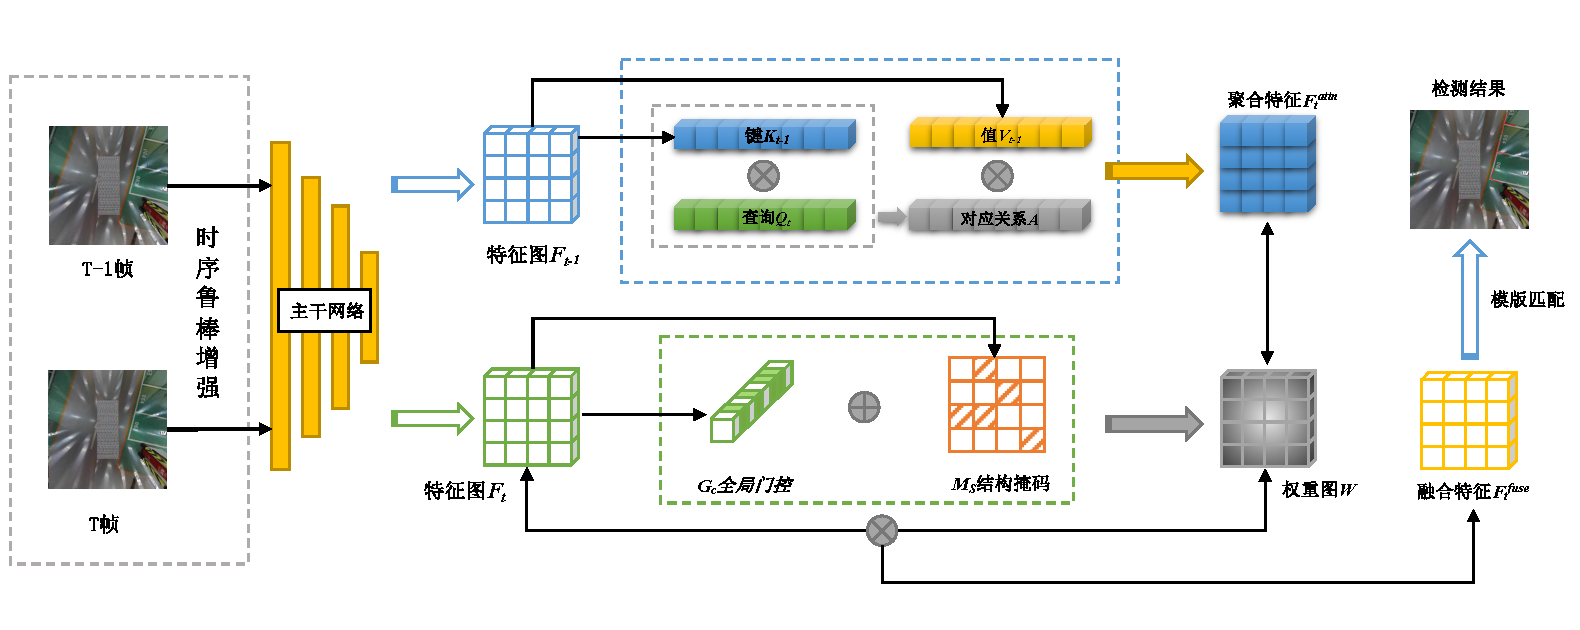
\includegraphics[width=1\textwidth]{figures/chp4/pipline_3.pdf}
\caption{多帧时序特征融合的停车位检测框架示意图 \\Fig~\ref{fig_pip3}~Overview of parking space detection method based on multi-frame temporal feature fusion}
\label{fig_pip3}
\end{figure}

\subsection{跨时帧自注意力}

在自动泊车场景中，相邻视频帧之间具有较强的时序连续性，停车位的几何结构与空间布局在短时间内基本保持稳定。为充分利用这一时序先验信息，本文提出跨帧自注意力机制，用于在特征层面实现多帧时序信息的自适应融合，增强当前帧对停车位结构的表征能力。

设当前帧与前一帧提取的特征分别为
$\mathbf{F}_t \in \mathbb{R}^{B \times C \times H \times W}, \quad
\mathbf{F}_{t-1} \in \mathbb{R}^{B \times C \times H \times W}$,
其中 B 表示批量大小，C 为通道数，H 与 W 为空间分辨率。跨帧自注意力模块以当前帧特征作为查询项，以前一帧特征作为键和值，通过注意力机制显式建模两帧之间的空间关联关系。

首先，采用 $1\times1$ 卷积对输入特征进行线性映射，分别生成查询（Query）、键（Key）和值（Value）：
$\mathbf{Q} = \phi_q(\mathbf{F}_t), \quad
\mathbf{K} = \phi_k(\mathbf{F}_{t-1}), \quad
\mathbf{V} = \phi_v(\mathbf{F}_{t-1})$,
其中 $\phi_q(\cdot)$、$\phi_k(\cdot)$ 和 $\phi_v(\cdot)$ 表示可学习的线性投影。为提升模型对不同语义子空间的建模能力，将通道维度划分为 N 个注意力头，并将空间维度展开为 HW，得到：
$\mathbf{Q}, \mathbf{K}, \mathbf{V} \in \mathbb{R}^{B \times N \times \frac{C}{N} \times HW}$.


在每一个注意力头中，采用缩放点积注意力计算当前帧与前一帧之间的相关性：
\begin{equation}
\mathbf{A} = \mathrm{Softmax}(\frac{\mathbf{Q}\mathbf{K}^{\top}}{\sqrt{C/N}}),
\end{equation}

其中 $\mathbf{A}$ 表示当前帧中每一个空间位置对前一帧各位置的注意力权重。该权重刻画了跨帧特征在空间维度上的对应关系，使模型能够自适应地关注历史帧中与当前帧最相关的区域。

基于计算得到的注意力权重，对前一帧的值特征进行加权求和，实现跨帧信息的聚合：
\begin{equation}
\mathbf{F}_{t}^{\mathrm{attn}} = \mathbf{A} \cdot \mathbf{V}
\end{equation}
随后，将多头特征在通道维度上进行拼接，并恢复为原始空间结构，得到融合后的特征表示:
\begin{equation}
\mathbf{F}_{t}^{\mathrm{attn}} \in \mathbb{R}^{B \times C \times H \times W}.
\end{equation}
最后，通过一个 $1\times1$ 卷积对融合特征进行线性变换，进一步整合跨帧信息并增强特征表达能力。

通过上述跨帧自注意力机制，模型能够在特征层面充分利用时序上下文信息，在当前帧特征受遮挡、光照变化或噪声干扰的情况下，仍可从历史帧中补充稳定可靠的停车位结构信息，从而提升停车位检测在复杂场景下的鲁棒性与时序一致性。


\subsection{动态时序融合}
在跨帧自注意力模块中，模型已能够从历史帧中提取与当前帧高度相关的时序信息。然而，不同场景下当前帧与历史帧的可靠性并不一致：在结构清晰、无遮挡的情况下，当前帧特征更具判别性；而在光照突变、遮挡或噪声干扰较强的场景中，历史帧特征往往更加稳定。若对两者进行静态或固定比例的融合，容易引入冗余信息甚至错误引导。

为此，本文进一步提出动态结构感知的时序融合模块，通过联合建模全局通道重要性与局部结构显著性，自适应地调节当前帧特征与跨帧注意力特征之间的融合权重，实现更加稳健的多帧特征整合。

设当前帧特征为
$\mathbf{F}_t \in \mathbb{R}^{B \times C \times H \times W}$,
跨帧自注意力模块输出的历史帧增强特征为
$\mathbf{F}_{t}^{\text{attn}} \in \mathbb{R}^{B \times C \times H \times W}$.
动态融合模块首先从当前帧特征中提取全局通道权重，用以刻画不同语义通道在当前时刻的重要程度。具体而言，通过全局平均池化将空间信息压缩为通道描述向量：
$\mathbf{g} = \text{GAP}(\mathbf{F}_t)$,
并经由 $1\times1$ 卷积与 Sigmoid 函数得到通道级门控权重：
\begin{equation}
\mathbf{G}_c = \sigma\!\left( W_c \mathbf{g} \right),
\quad
\mathbf{G}_c \in \mathbb{R}^{B \times C \times 1 \times 1}
\end{equation}
该权重反映了不同通道在当前帧中的全局响应强度，有助于抑制低置信度语义特征。

与此同时，为突出停车位结构相关的空间区域，模块进一步从当前帧特征中预测结构感知掩码。该掩码通过一组卷积操作生成：
\begin{equation}
\mathbf{M}_s = \sigma\!\left( W_2 \, \delta \!\left( \text{BN}( W_1 * \mathbf{F}_t ) \right) \right),
\quad
\mathbf{M}_s \in \mathbb{R}^{B \times 1 \times H \times W}
\end{equation}
其中 $*$ 表示卷积操作，$\delta(\cdot)$ 为 ReLU 激活函数，$\mathbf{M}_s$ 表示空间维度上的结构显著性权重。该掩码能够自适应地关注停车位边线、角点等关键结构区域，同时弱化背景区域对时序融合的干扰。

随后，将通道级权重与空间结构掩码进行联合建模，通过广播机制得到最终的动态融合权重：
\begin{equation}
\mathbf{W} = \mathbf{G}_c \odot \mathbf{M}_s,
\quad
\mathbf{W} \in \mathbb{R}^{B \times C \times H \times W},
\end{equation}

其中 $\odot$ 表示逐元素乘法。基于该动态权重，当前帧特征与历史帧增强特征按照如下方式进行融合：
\begin{equation}
\mathbf{F}_{t}^{\mathrm{fuse}} =
\mathbf{W} \odot \mathbf{F}_{t}^{\text{attn}}
+ \left( 1 - \mathbf{W} \right) \odot \mathbf{F}_t.
\end{equation}

通过这种动态融合方式，模型能够根据当前场景的结构清晰度和稳定性，自适应地平衡历史信息与当前信息的贡献。在结构清晰的区域，模型更多依赖当前帧特征；在结构模糊或受干扰的区域，则更多参考历史帧的稳定信息，从而实现更稳健的时序特征融合。

上述融合策略使模型能够在空间和通道两个层面上自适应地平衡当前帧与历史帧信息：在结构显著且语义稳定的区域，更倾向于引入跨帧增强特征；而在当前帧信息可靠的区域，则保留更多当前帧特征，从而避免时序信息的过度引入。
通过引入该动态结构感知时序融合模块，模型不仅提升了多帧特征融合的灵活性，还显著增强了在复杂场景下停车位检测的鲁棒性，为后续关键点检测与结构匹配提供了更加稳定且一致的特征表示。




\subsection{时序鲁棒增强}
在多帧时序停车位检测任务中，模型不仅需要学习跨帧特征之间的关联关系，还需要具备对真实驾驶场景中复杂扰动的鲁棒性。在实际应用中，相邻帧之间往往存在亮度变化、噪声干扰、运动模糊以及局部遮挡等非理想因素，若训练阶段未显式考虑这些时序扰动，模型容易对帧间细微变化产生过拟合，从而削弱时序融合模块的有效性。

为此，本文提出时序鲁棒增强策略，在不改变停车位关键点空间坐标的前提下，对相邻帧施加具有物理合理性的图像扰动，模拟真实视频序列中的帧间差异，引导模型学习更加稳健的时序特征表示。该策略在训练阶段对前一帧与当前帧图像进行联合与差异化增强，同时严格保证几何一致性，避免对关键点标注产生破坏。

设前一帧与当前帧原始图像分别为
$\mathbf{I}_{t-1} (\mathbf{I}_t \in \mathbb{R}^{H \times W \times 3})$,
对应的停车位关键点标注为
$\mathcal{P}_t = \{ \mathbf{p}_i \}_{i=1}^{N}$.
时序鲁棒增强的核心原则是在增强过程中保持关键点坐标不变，即增强操作满足：
\begin{equation}
\mathcal{T}(\mathbf{p}_i) = \mathbf{p}_i
\end{equation}
从而保证监督信号在空间上的一致性。

在此约束下，本文首先对相邻帧施加同步光度增强，以模拟环境光照在短时间内的整体变化。具体而言，对两帧图像同时进行亮度与对比度扰动以及轻微高斯模糊处理：
\begin{equation}
\mathbf{I}'_{t-1} = \mathcal{A}_{\text{sync}}(\mathbf{I}_{t-1}), \quad
\mathbf{I}'_{t} = \mathcal{A}_{\text{sync}}(\mathbf{I}_{t})
\end{equation}
该操作保持帧间一致性，有助于模型学习对全局光照变化的不变性。

随后，为模拟真实视频中由曝光变化、传感器噪声或运动引起的帧间差异，仅对当前帧施加非同步光度与退化增强：
\begin{equation}
\tilde{\mathbf{I}}_{t} = \mathcal{A}_{\text{diff}}(\mathbf{I}'_{t}),
\end{equation}
其中 $\mathcal{A}_{\text{diff}}(\cdot)$ 包括亮度与对比度微扰、加性高斯噪声、方向性运动模糊以及 JPEG 压缩伪影等操作。该设计刻意引入前后帧之间的视觉差异，从而逼迫模型在时序融合过程中学会区分结构性信息与瞬时噪声。

此外，为增强模型在遮挡场景下的鲁棒性，本文在当前帧中进一步引入局部随机遮挡增强，通过在随机位置生成若干矩形遮挡区域：
\begin{equation}
\tilde{\mathbf{I}}_{t}(x, y) =
\begin{cases}
\mathbf{r}, & (x,y) \in \Omega_{\text{occ}} \\
\tilde{\mathbf{I}}_{t}(x, y), & \text{otherwise}
\end{cases}
\end{equation}
其中 $\Omega_{\text{occ}}$ 表示遮挡区域，$\mathbf{r}$ 为随机颜色值。该操作模拟车辆、行人或环境物体对停车位边线的局部遮挡，有助于模型利用时序上下文补偿缺失信息。

最后，对当前帧施加轻微的颜色扰动，以 HSV 空间中的饱和度与色调变化形式体现，从而进一步模拟复杂环境下的成像差异。经过上述增强处理后，得到最终用于训练的时序输入对：
\begin{equation}
(\hat{\mathbf{I}}_{t-1}, \hat{\mathbf{I}}_{t}, \mathcal{P}_t)
\end{equation}
其中关键点标注 $\mathcal{P}_t$ 在整个增强过程中保持不变。

通过引入该时序鲁棒增强策略，模型在训练阶段能够充分暴露于多种合理的帧间扰动情形，从而在推理阶段更加依赖结构一致性与时序上下文信息，而非单帧的局部外观特征。这一策略与跨帧自注意力模块及动态结构感知融合模块形成互补，有效提升了多帧停车位检测方法在复杂真实场景下的泛化能力与稳定性。


\section{实验结果及分析}

\subsection{时序数据集PSTD}

为系统评估所提多帧时序停车位检测方法在连续场景下的性能，本文基于CRPS-D数据集构建了专用于时序建模的连续帧数据集，命名为PSTD。CRPS-D是面向复杂真实场景的大规模停车位关键点检测数据集，覆盖多种光照条件、天气环境及停车位布局形式，具有停车位密度高、结构多样性强等特点，能够充分反映实际自动泊车场景中的挑战性因素。PSTD数据集从CRPS-D中筛选并整理具有明确时间连续关系的图像序列，重点用于验证跨帧特征建模与时序鲁棒增强策略的有效性。
\begin{figure}[!h]
\centering
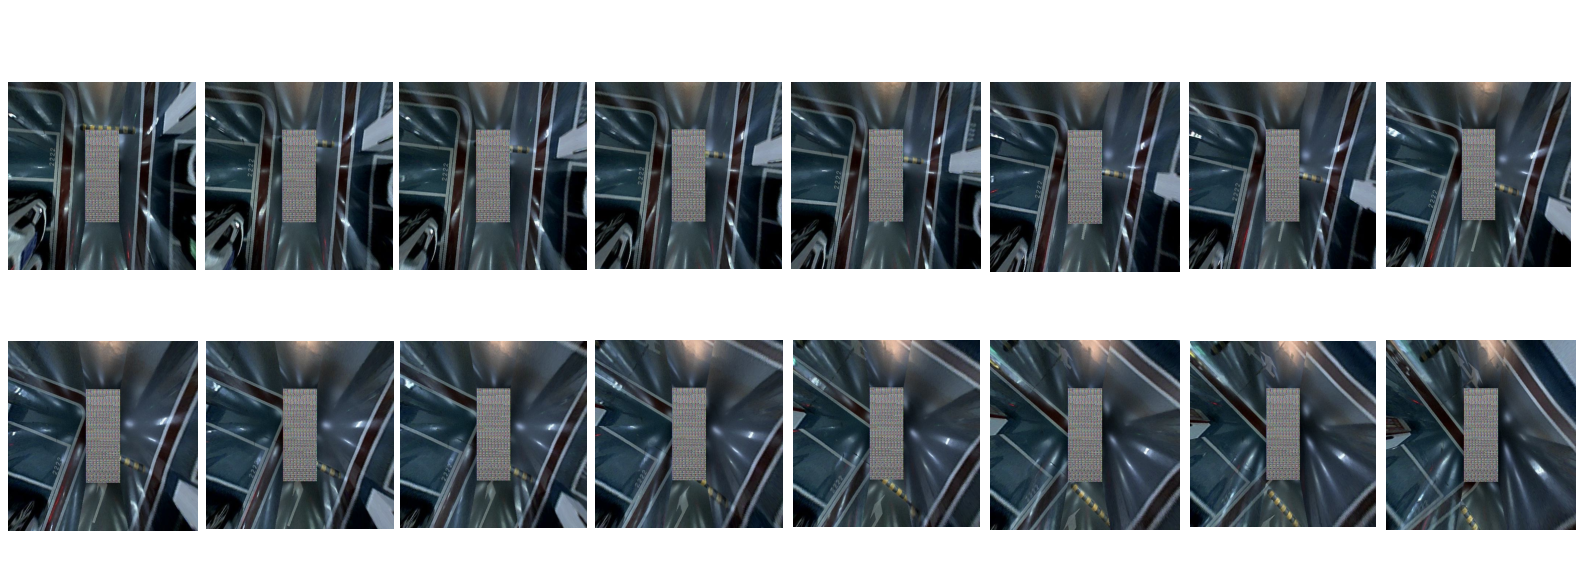
\includegraphics[width=1\textwidth]{figures/chp4/pstd.pdf}
\caption{PSTD数据集部分示例图片 \\Fig~\ref{fig_pstd}~Sample images from the PSTD dataset}
\label{fig_pstd}
\end{figure}

PSTD 数据集中的样本均由同一采集设备在短时间间隔内连续获取，相邻帧之间视角变化较小，停车位的空间结构整体保持一致，但在光照条件、局部遮挡、成像噪声及运动模糊等方面存在自然变化，能够较好地模拟真实自动泊车场景中的视频输入特性。如图\ref{fig_pstd}所示。在数据构建过程中，本文以当前帧作为监督目标帧，并选取其前一帧作为历史参考帧，形成二帧时序输入对：
\begin{equation}
(\mathbf{I}_{t-1}, \mathbf{I}_{t})
\end{equation}
其中仅对当前帧 $\mathbf{I}_{t}$ 使用原始 CRPS-D 数据集中的停车位关键点标注作为监督信号，从而避免跨帧标注不一致问题。

在保证标注精度与空间一致性的前提下，PSTD 数据集未对关键点坐标进行任何几何变换或插值处理，所有样本均直接继承 CRPS-D 的人工标注结果。同时，数据集中允许存在一定程度的帧间退化差异，以增强数据对复杂真实场景的代表性。

在实验设置中，PSTD 数据集共包含 8990 组连续帧样本，其中 7192 组用于训练，1798 组用于测试。训练集与测试集在场景类型、光照条件及停车位布局等方面保持一致分布，确保实验结果具有公平性与可比性。

通过构建 PSTD 时序数据集，本文在保留 CRPS-D 原有高复杂度与多样性的基础上，引入了明确的时间维度，为多帧时序特征融合方法的有效性验证提供了可靠的数据支撑。


\subsection{对比实验}
为验证所提出方法的有效性，本节在数据集PSTD上进行了充分的对比实验。
表 \ref{tab_pstc} 给出了本文方法与近期代表性停车位检测方法在 PSTD 时序数据集上的对比结果。由于现有停车位检测研究主要集中于单帧图像场景，当前该领域尚不存在公开可用的时序停车位检测数据集，因此本文仅能基于自构建的 PSTD 数据集开展时序对比实验。为保证对比的公平性与可复现性，本文选取具有公开实现的代表性方法，并在 PSTD 数据集上重新训练与测试其模型性能。

从实验结果可以看出，本文方法在查准率(Precision)、查全率(Recall)以及平均精度（AP）三项指标上均取得了最优表现。与基于图结构建模的 GCN 方法相比，本文方法在 AP 指标上提升了 +9.77\%，表明引入时序信息后，模型在复杂场景下对停车位结构的整体识别能力得到了显著增强。相较于 DMPR-PS 方法，本文方法在 查准率和查全率 上分别提升了 +0.96\% 和 +0.39\%，同时 AP 提升 +2.01\%，说明所提出的跨帧特征建模与动态时序融合策略能够在保持高召回率的同时，有效减少误检情况。

需要指出的是，尽管上述对比方法原本设计用于单帧停车位检测任务，但在 PSTD 数据集上的重新训练结果仍能够作为合理的对比基线，用于评估不同方法在连续帧场景下的检测性能。实验结果表明，单帧方法在面对帧间退化与遮挡时存在一定性能瓶颈，而本文提出的多帧时序停车位检测方法通过跨帧自注意力建模、动态结构感知融合以及时序鲁棒增强策略，能够更充分地利用时序上下文信息，从而在连续场景下取得更加稳定且准确的检测效果。

\begin{table}[!h]
\centering
\setlength{\tabcolsep}{8mm}
\caption{与开源SoTA方法对比\\
Table~\ref{tab_pstc}~Comparison with open-source SoTA methods}
\begin{tabular}{lccccc}
\toprule
    方法 &  Precision & Recall &  AP\\
\midrule
       GCN\cite{min2021attentional}  &  87.00\%	& 86.44\%	& 82.20\% \\
       DMPR-PS\cite{huang2019dmpr} &  91.57\%	& 91.94\%	& 89.96\% \\
       \textbf{Ours} &   \textbf{92.53\%} & \textbf{92.33\%} & \textbf{91.97\%}\\
\bottomrule
\end{tabular}
\label{tab_pstc}
\end{table}


\subsection{消融实验}

表 \ref{tab_3ab} 给出了本文所提出多帧时序停车位检测方法的消融实验结果。实验以单帧停车位检测模型作为基线，在此基础上逐步引入跨帧自注意力、动态时序融合以及时序鲁棒增强模块，以分析各个组成模块对整体检测性能的影响。

从实验结果可以看出，当仅使用单帧模型时，平均精度$AP$ 为 89.96\%。在此基础上引入跨帧自注意力模块后，模型性能提升至 91.46\%，取得了最为显著的性能增益。这一结果表明，通过显式建模相邻帧之间的特征关联关系，模型能够有效利用时序上下文信息，从而显著提升停车位结构的整体检测精度。

进一步加入动态时序融合模块后，$AP$ 提升至 91.71\%。该模块通过自适应调节当前帧与历史帧特征之间的融合权重，在抑制噪声干扰的同时增强结构一致性，从而在已有时序建模基础上进一步提升模型性能。

当三种时序相关模块全部引入后，模型取得了最高的 $AP$ 为 91.97\%。该结果验证了时序鲁棒增强策略在训练阶段对模型泛化能力的积极作用，使模型在面对光照变化、噪声干扰及局部遮挡等复杂情况时仍能保持稳定的检测表现。

综合消融实验结果可以看出，本文提出的跨帧自注意力、动态时序融合及时序鲁棒增强三种设计在性能提升方面具有良好的互补性，共同构成了一个有效且稳健的多帧时序停车位检测框架。


\begin{table*}[!h]
\centering
\setlength{\tabcolsep}{3mm}
\caption{消融实验结果 \\
Table~\ref{tab_3ab}~Results of ablation study}
\small
\begin{tabular}{ccccc}
\toprule
    Baseline(单帧) & 跨帧自注意力 & 动态时序融合  & 时序鲁棒增强 &  $AP$ \\
\midrule
    \checkmark  &  &  &  &  89.96\% \\
     \checkmark & \checkmark &  &  &  91.46\% \\
     \checkmark & \checkmark & \checkmark &  &  91.71\% \\
     \checkmark & \checkmark & \checkmark & \checkmark  & \textbf{91.97\%} \\
\bottomrule
\end{tabular}
\label{tab_3ab}
\end{table*}


\subsection{推理速度实验}

在推理效率方面，本文对比了所提出方法与两种代表性方法在 GPU 平台上的单帧推理时间，如表 \ref{tab_infer} 所示。DMPR 在 Nvidia Titan Xp 上的推理时间为 10 ms，表现出较高的推理效率；GCN 方法由于引入了图结构建模与复杂的节点关系推理，其单帧推理时间显著增加，达到 49 ms。相比之下，本文方法在 Nvidia 2080Ti 上的推理时间为 25 ms，整体处于合理区间。

尽管不同方法的测试平台存在一定差异，但从结果可以看出，本文方法在引入时序特征建模与结构感知机制的前提下，仍能够保持较为可控的推理开销。与基于图结构的 GCN 方法相比，本文方法显著降低了推理延迟；相较于纯单帧方法 DMPR-PS，推理时间有所增加，但换来了更强的时序一致性建模能力与整体检测性能提升。综合来看，本文方法在推理效率与检测精度之间取得了较为合理的平衡，具备在实际自动泊车场景中部署的潜力。

\begin{table}[!h]
\centering
\setlength{\tabcolsep}{10mm}
\caption{推理效率对比 \\
Table~\ref{tab_infer}~Comparison of inference efficiency}
\setlength{\tabcolsep}{10mm}
\begin{tabular}{lcc}
\toprule
   模型 & GPU型号 & 推理速度 \\
\midrule
    DMPR-PS\cite{huang2019dmpr} & Nvidia Titan Xp & 10ms \\
    GCN\cite{min2021attentional} & Nvidia Titan Xp & 49ms \\
    ours & Nvidia 2080Ti & 25ms \\
     
\bottomrule
\end{tabular}
\label{tab_infer}
\end{table}

此外，本文将训练好的模型部署至配备神经处理单元（Neural Processing Unit, NPU）的车规级处理器上，并在真实车辆平台上进行了在线推理测试。如图\ref{fig_intel}所示， 本文使用智能停车系统，将在 PSTD 数据集上训练的模型集成到该系统中。该系统在检测到可用停车位后，可以自动引导车辆进入停车位。实验结果表明，该模型在实际车载环境中能够稳定运行，推理帧率可达到约 \textbf{30 FPS}，验证了所提出方法在资源受限硬件条件下的实时性与工程可行性，能够满足低速自动泊车场景对感知算法的时序响应需求。


\begin{figure}[!h]
\centering
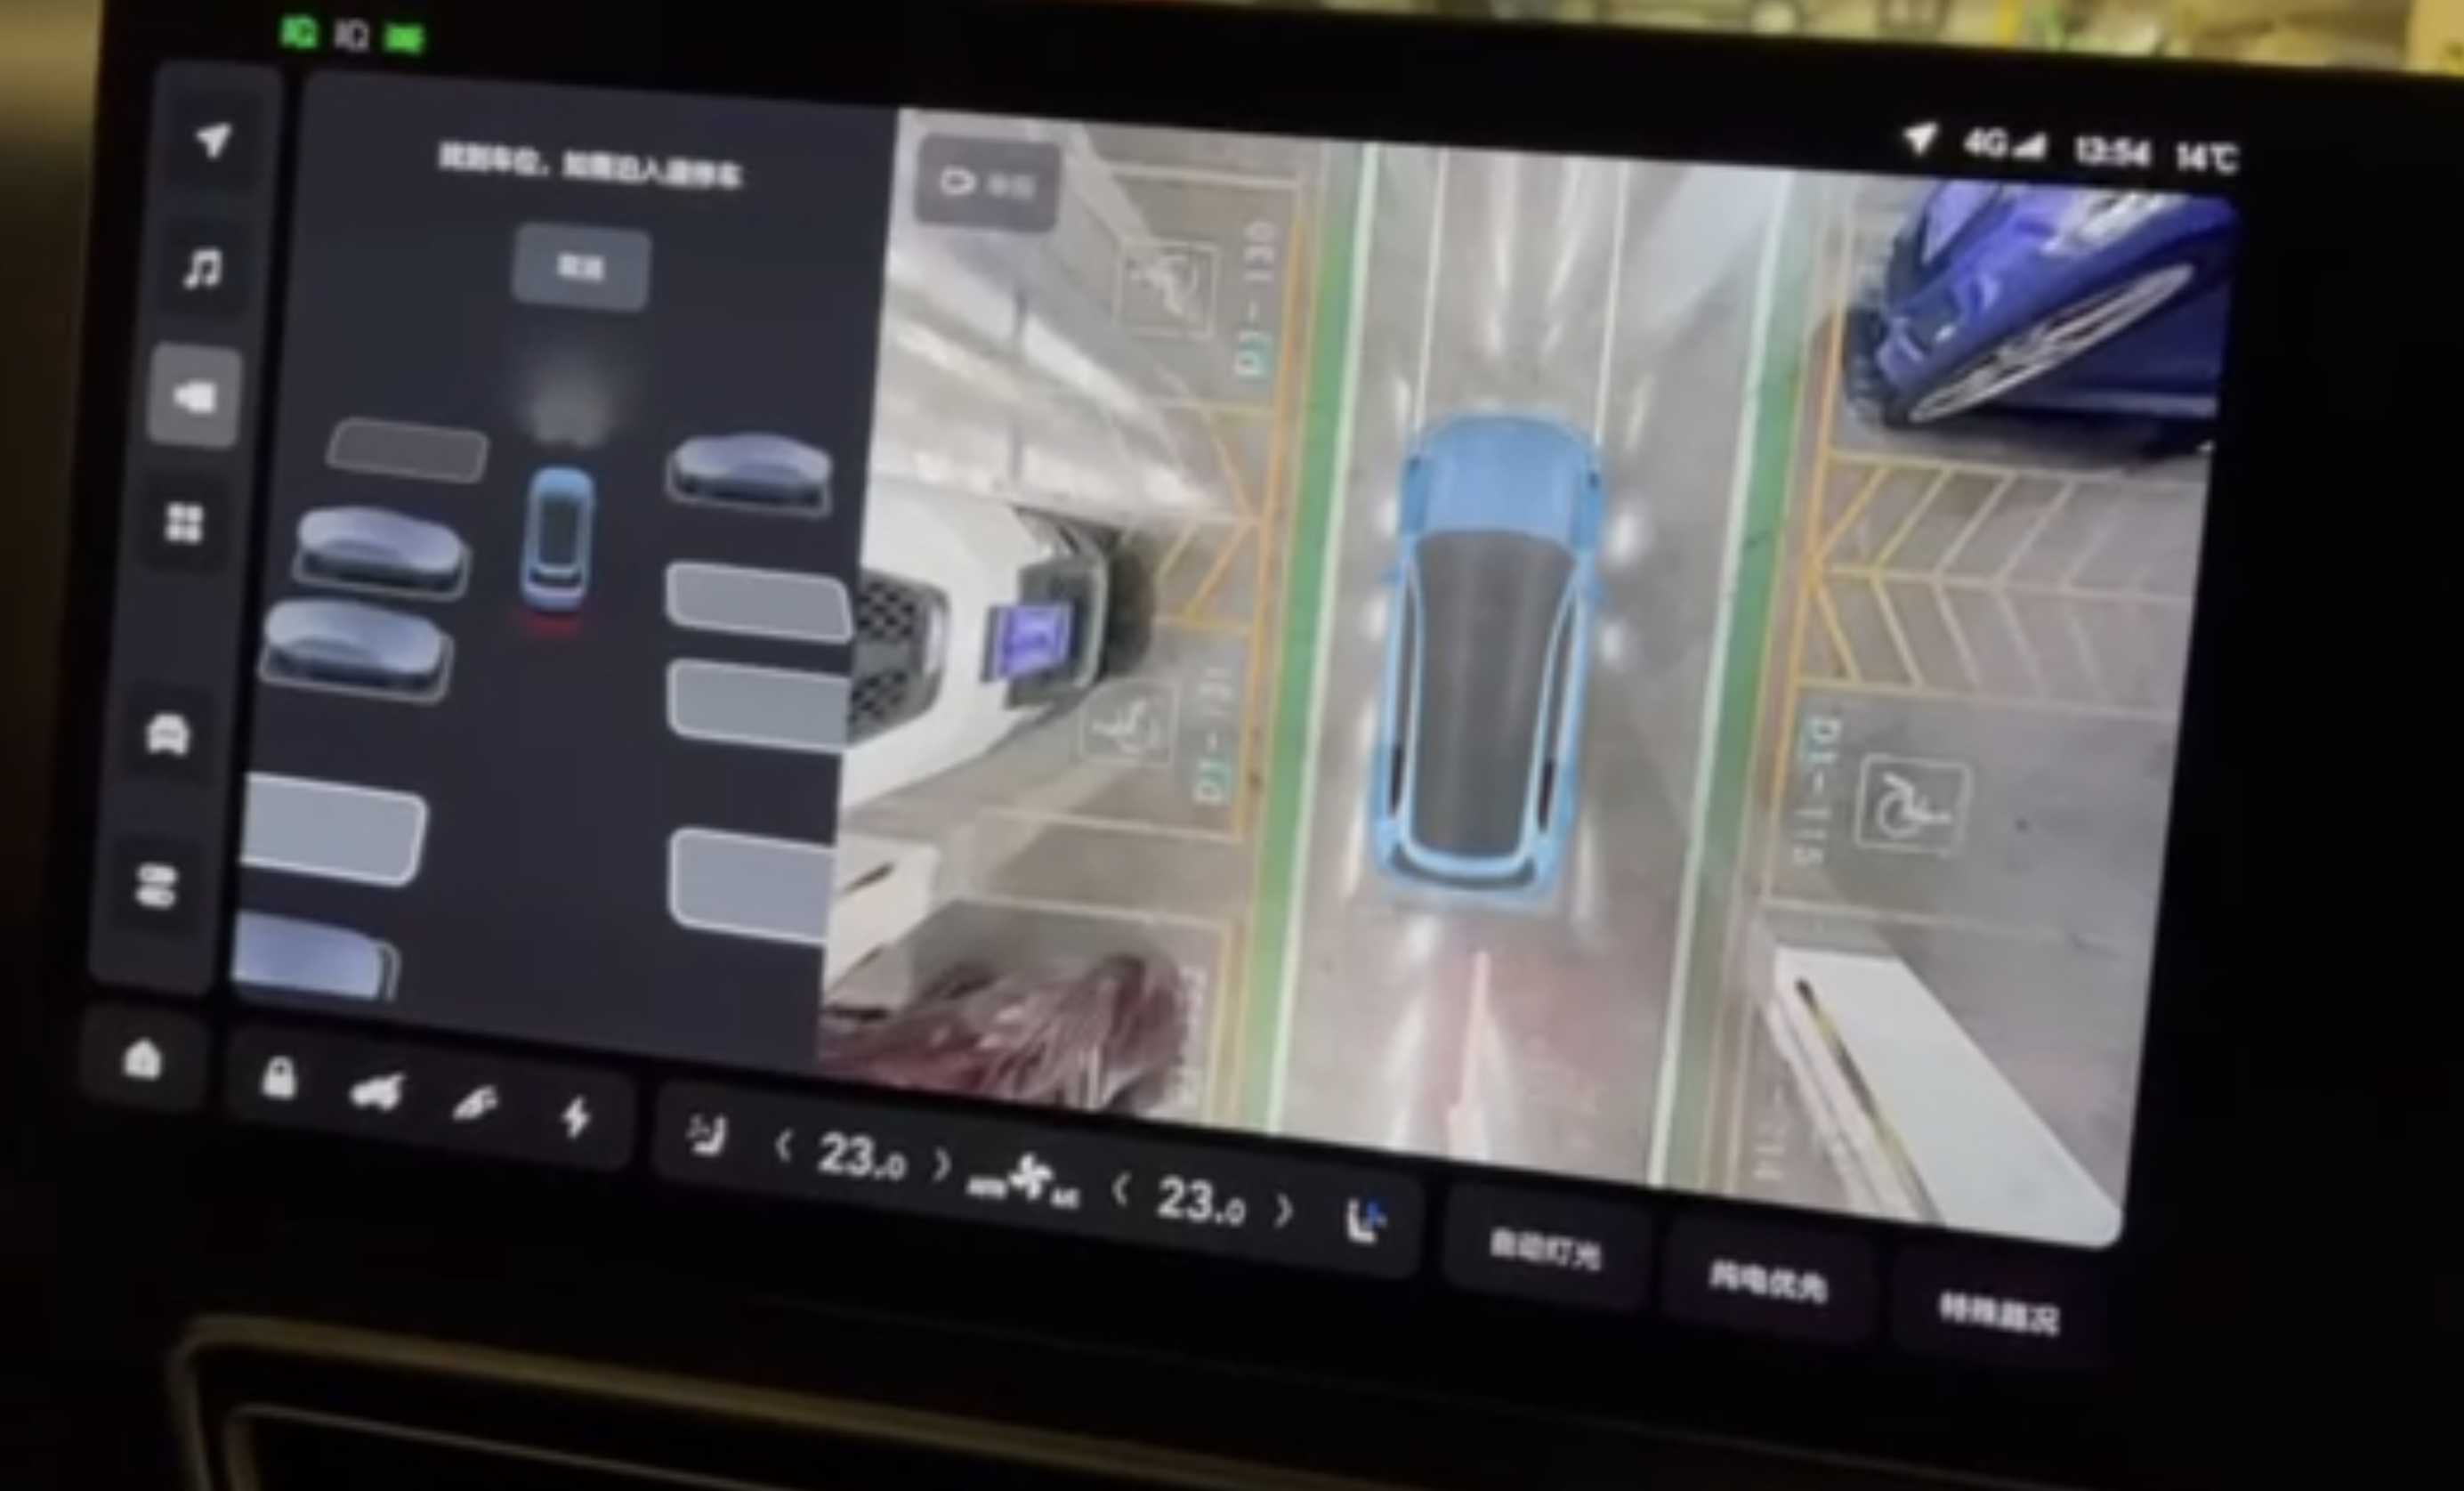
\includegraphics[width=1\textwidth]{figures/chp4/example.png}
\caption{智能停车系统 \\Fig~\ref{fig_intel}~Intelligent parking system}
\label{fig_intel}
\end{figure}


\section{本章小结}

在第二章单帧结构感知检测方法的基础上，本章进一步面向真实驾驶场景中连续帧输入条件下的检测稳定性问题，提出了一种多帧时序特征融合的停车位检测方法。该方法通过融合相邻帧之间的时序信息，有效缓解了单帧检测中由于瞬时遮挡、光照变化或视角抖动带来的不确定性。

首先，为充分利用连续帧之间的时序信息，提出了跨帧自注意力模块，通过显式建模当前帧与前一帧的空间特征关联关系，实现了跨帧信息的有效聚合。该模块能够增强模型在局部遮挡、光照变化及噪声干扰情况下对停车位结构的辨识能力，是时序建模的核心组成部分。

其次，提出了动态结构感知的时序融合模块，通过联合建模全局通道重要性与局部结构显著性，自适应地调节当前帧与历史帧特征的融合权重。这一设计能够在不同场景下合理平衡单帧信息与跨帧增强信息，进一步提高检测的稳定性与精度。

第三，为增强模型在复杂真实场景下的泛化能力，引入了时序鲁棒增强策略，在训练阶段对连续帧施加光度变化、噪声扰动、运动模糊及局部遮挡等增强操作，同时保持停车位关键点空间一致性。该策略使模型在面对帧间退化和环境扰动时仍能保持稳健性能。

在数据方面，本文基于 CRPS-D 构建了PSTD 时序数据集，为连续帧停车位检测提供了可靠的数据支撑，填补了该领域缺乏开源时序数据集的空白。通过系统的实验验证，包括对比实验和消融研究，结果表明本文方法在 Precision、Recall 以及 AP 指标上均优于现有方法，充分证明了跨帧建模、动态融合以及鲁棒增强三者的互补性与有效性。


总之，本章提出的方法在理论设计与实践验证上均显示出良好的性能，为多帧时序停车位检测提供了一种可行且高效的解决方案，同时为未来进一步研究连续场景下的智能交通感知任务奠定了基础。通过将停车位检测从单帧空间结构建模扩展至多帧时序建模，本章方法在保持端到端推理流程的同时，进一步提升了检测结果在时间维度上的一致性与鲁棒性，使所提出的停车位检测方法更加贴近实际应用场景。 								%第四章
	%  \setlength{\baselineskip}{20pt}
\chapter{总结与展望}
\label{cha:chap5}



\section{研究总结}

我这里更关注的是问题建模方式的变化。
第二章将停车位检测从基于规则的检测流程重构为结构感知的端到端建模问题；
第三章则在此基础上，将建模维度由单帧空间结构扩展到多帧时序一致性建模，因此并不是简单的模块叠加，而是检测范式在空间和时间维度上的逐步扩展。

创新点一：构建大规模复杂场景停车位数据集并提出半监督检测框架

针对现有停车位检测研究中高质量标注数据匮乏、复杂场景覆盖不足的问题，本文构建了一个覆盖多光照、多视角、多停车形式的大规模停车位数据集，显著提升了数据的多样性与复杂性。在此基础上，提出了一种面向停车位检测任务的半监督检测框架，通过教师–学生学习范式有效利用未标注数据，缓解了标注成本高昂对模型训练与泛化能力的制约，为后续检测方法的研究提供了统一且可靠的数据与训练基础。

创新定性关键词：
数据层创新 + 学习范式创新


创新点二：提出单帧结构感知的端到端停车位检测方法

针对传统停车位检测方法中依赖启发式规则进行后处理匹配、结构一致性难以保证的问题，本文提出了一种单帧结构感知的端到端停车位检测方法。该方法从建模角度将停车位检测问题重构为基于关键点的结构化预测问题，在端到端训练过程中显式引入停车位内部结构关系约束，使结构一致性直接参与模型优化，从而避免了规则依赖并提升了复杂与密集场景下的检测稳定性与一致性。

创新定性关键词：
问题建模重构 + 结构感知 + 端到端优化

创新点三：提出多帧时序特征融合的停车位检测方法

针对真实驾驶场景中停车位检测结果在连续帧条件下易受遮挡、视角变化和噪声影响而不稳定的问题，本文在单帧结构感知检测方法的基础上，进一步提出了一种多帧时序特征融合的停车位检测方法。该方法通过对连续帧中的结构感知表示进行时序建模，将停车位检测从静态空间结构建模扩展至时空联合建模，有效提升了检测结果在时间维度上的一致性与鲁棒性，使所提出的方法更加贴近实际应用需求。

创新定性关键词：
建模维度扩展 + 时序一致性建模


本文围绕复杂场景下停车位检测任务，从数据与学习范式、单帧结构建模以及多帧时序建模三个层面展开研究，逐步将停车位检测从基于规则的静态检测流程，发展为结构感知且具备时序一致性的端到端检测方法


\section{未来展望}
 								%第五章




	\nocite{*}
	\bibliography{reference/ref}

     \backmatter




	%\mmchapter{作者简历}
 \setlength{\baselineskip}{16pt}
\chapter{作者简历及攻读硕士学位期间取得的研究成果}\zihao{5}
\setlength{\parindent}{0pt}

%[内容采用五号宋体]  包括教育经历、工作经历、攻读学位期间发表的论文和完成的工作等。行距16磅，段前后各为0磅。

一、作者简历


2019年9月 至 2023年6月，就读于北京交通大学，计算机科学与技术学院，计算机科学与技术专业，获学士学位；

2023年9月 至 2026年6月，就读于北京交通大学，计算机科学与技术学院，人工智能专业，获硕士学位；


\vspace{10pt}
二、发表论文

[1] \textbf{Zhang Z}, Lin C, Nie L, et al. Advancing Real-World Parking Slot Detection With Large-Scale
Dataset and Semi-Supervised Baseline [J]. IEEE Transactions on Intelligent Transportation Systems, 2025.(本人一作, CCF-B, JCR Q1, 中科院二区TOP)


\vspace{10pt}
三、参与科研项目

[1] 鱼眼图像处理的关键技术研究，国家自然科学基金

[2] 智能驾驶场景下的自动标注关键技术研究，毫末智行科技有限公司


\vspace{10pt}
四、参与竞赛项目

[1] 第五届“华为杯”中国研究生人工智能创新大赛（2023）   国家级二等奖

[2] 第十九届“挑战杯”全国大学生课外学术科技作品竞赛（2024）   国家级二等奖



\vspace{10pt}
五、获奖情况

   [1] 一等学业奖学金，北京交通大学，2023
   
   [2] 一等学业奖学金，北京交通大学，2024

   [3] 硕士研究生国家奖学金，中华人民共和国教育部，2025



	\include{chapters/statement} 	

      \setlength{\baselineskip}{16pt}
\chapter{学位论文数据集}\zihao{-4}


\setcounter{table}{0}
\renewcommand{\thetable}{1.\arabic{table}}

\begin{table}[!h]

\small 
\centering
\caption{数据集页}
\begin{tabular}{|p{2.6cm}|p{2.6cm}|p{2.5cm}|p{2.9cm}|p{2.5cm}|}
\hline
%\multirow{2}{*}{1} & \multicolumn{2}{|c|}{1} \\
%\cline{2-3}
%& 1 & 1 \\
%\hline
%1 & \multicolumn{2}{|c|}{1}\\
关键词$^*$  & 密级$^*$ & 中图分类号 & UDC & 论文资助 \\
\hline
    停车位检测；数据集；半监督学习；关键点检测；结构感知；时序建模     &  公开 &            &     &          \\  %对应上一行的标题对应填写： 关键词、密级、中图分类号、UDC、论文资助
\hline

\multicolumn{2}{|p{5.4cm}|}{学位授予单位名称$^*$} & 学位授予单位代码$^*$ & 学位类别$^*$ &  学位级别$^*$    \\
\hline
\multicolumn{2}{|p{5.4cm}|}{北京交通大学 }        &  10004               &      电子信息        &        硕士          \\%对应上一行的标题对应填写: 学位类别、学位级别
\hline

\multicolumn{2}{|p{5.4cm}|}{论文题名$^*$} & \multicolumn{2}{p{5.4cm}|}{并列题名$^*$} &  论文语种$^*$    \\
\hline
\multicolumn{2}{|p{5.4cm}|}{ 面向复杂真实场景的停车位检测技术研究  }          & \multicolumn{2}{p{5.4cm}|}{ Research on Parking Slot Detection Techniques for Complex Real-World Scenarios }        &   中文   \\ %对应上一行的标题对应填写: 论文题目、并列题名、论文语种
\hline

作者姓名$^*$    &  \multicolumn{2}{p{5.4cm}|}{ 张志浩 }   & 学号$^*$  &  23125344   \\%在对应空格上填写：作者姓名，学号 
\hline

\multicolumn{2}{|p{5.4cm}|}{ 培养单位名称$^*$ }  &  培养单位代码$^*$   & 培养单位地址  &  邮编   \\
\hline
\multicolumn{2}{|p{5.4cm}|}{ 北京交通大学 }  &  10004   & 北京市海淀区西直门外上园村3号  &  100044   \\
\hline

\multicolumn{2}{|p{5.4cm}|}{ 专业学位类别（领域）$^*$ }  &  研究方向$^*$   & 学制$^*$  & 学位授予年$^*$   \\
\hline
\multicolumn{2}{|p{5.4cm}|}{ 人工智能 }              &       停车位检测          &     3年      &   2026   \\%对应上一行的标题对应填写:学科专业、 研究方向、学制、学位授予年

\hline
论文提交日期 $^*$    & \multicolumn{4}{l|}{ 2026年6月 }   \\%在对应空格上填写：论文提交日期 
\hline

 导师姓名$^*$    &  \multicolumn{2}{p{5.4cm}|}{ 林春雨 }   & 职称$^*$  &   教授  \\%在对应空格上填写： 导师姓名、职称
\hline

 评阅人    &  \multicolumn{2}{p{5.4cm}|}{ 答辩委员会主席$^*$ }   & \multicolumn{2}{p{5.4cm}|}{ 答辩委员会成员 } \\
\hline
\        &  \multicolumn{2}{p{5.4cm}|}{  黄雅平 }   & \multicolumn{2}{p{5.4cm}|}{ 刘真、黄惠芳  } \\%对应上一行的标题对应填写:评阅人、主席、成员
\        &  \multicolumn{2}{p{5.4cm}|}{   }   & \multicolumn{2}{p{5.4cm}|}{   } \\
\        &  \multicolumn{2}{p{5.4cm}|}{   }   & \multicolumn{2}{p{5.4cm}|}{   } \\

\hline
\multicolumn{5}{|p{15cm}|}{ 电子版论文提交格式 \; 文本（$\surd$） \; 图像（\hspace*{0.5em}）\; 视频（\hspace*{0.5em}）\;  音频（\hspace*{0.5em}）\; 多媒体（\hspace*{0.5em}）\; 其他（\hspace*{0.5em}）}  \\
\multicolumn{5}{|p{13.1cm}|}{ 推荐格式：application/msword; application/pdf }  \\

\hline
\multicolumn{2}{|p{5.4cm}|}{ 电子版论文出版（发布）者  } & \multicolumn{2}{p{5.4cm}|}{电子版论文出版（发布）地  } & 权限声明\\
\hline
\multicolumn{2}{|p{5.4cm}|}{   } & \multicolumn{2}{p{5.4cm}|}{   } &  \\ %对应上一行的标题对应填写: 电子版论文出版（发布）者、发布地

\hline
论文总页数 $^*$    & \multicolumn{4}{l|}{ 67 }   \\%在对应空格上填写：页数
\hline
\multicolumn{5}{|p{13.1cm}|}{ 共33项，其中带$*$为必填数据，为22项。 }  \\



\hline 
\end{tabular}	
\end{table}





















						


\end{document}




















